\documentclass[uplatex,dvipdfmx]{jsreport}
\title{力学的模型の理論}
\author{司馬博文 J4-190549}
\date{\today}
\pagestyle{headings} \setcounter{secnumdepth}{4}
\input{/Users/Hirofumi Shiba/NatureOfStatistics/preamble_no_fonts.tex}
%\input{/Users/hirofumi.shiba48/NatureOfStatistics/preamble_no_fonts.tex}
\usepackage[math]{anttor}
\begin{document}
\tableofcontents

\begin{abstract}
    数々の数理モデルの中で,時空間のモデルに使われるのは実数とこれがなすBanach空間$\R^n$であってきた.
    これを力学系=「連続な状態空間内であって,経時発展法則が微分方程式によって与えられるもの」という.
    確率空間や統計的実験が考えられるのは遥かに後のことである.
    力学系を解析する位相的・幾何学的・解析的手法を見る(微分方程式論という).
    そこに確率空間の構造を入れる量子確率論・情報理論,そして古典的問題の確率過程による解析までを見て,
    確率統計学的な示唆を得たい.
    ただし,統計力学は扱わない.
    \begin{enumerate}
        \item Hamiltonの正準方程式が定める力学系を\textbf{Hamilton力学系}という.測地流や流体力学の渦点流などの力学系も含む.
        \begin{enumerate}[(i)]
            \item Hamilton力学系が\textbf{完全積分可能}または\textbf{可積分系}であるとは,独立変数の数と同じ数の第一積分$F_1,\cdots,F_n$が存在して次を満たす場合をいう:
            \begin{enumerate}[(a)]
                \item $dF_1,\cdots,dF_n$は$M$の稠密な開集合上で線形独立.
                \item $\forall_{i,j\in[n]}\;[F_i,F_j]=0$.
            \end{enumerate}
            このとき,解は規則的でよくわかる(Liouvoille-Arnoldの定理).
            \item 可積分系を摂動すると一般には非可積分系になる(三体問題など)が,摂動が十分小さければ可積分系
            の時に存在していた規則的な解が同様に存在する.
            これをKAM定理という.
            Kolmogorov, Arnold, Moserによる.
        \end{enumerate}
        \item 力学では,状態空間をEuclid空間に取る.これは変数の空間であり,対象は多様体である.Lagrange以来の,運動を座標系の取り方に依らない理解への志向が結節した数学的対象である.
        一方で,セミパラメトリックモデルでは,変数の空間を一般のBanach空間に取ることになる.
    \end{enumerate}
\end{abstract}

\chapter{常微分方程式}

\begin{quotation}
    解析力学は微分方程式の解法理論という性格もある.
\end{quotation}

\begin{notation}\mbox{}
    \begin{enumerate}
        \item $B^d\subset\R^d$を任意の閉球とする.$B$をBanach空間$X$の任意の閉球とする.
    \end{enumerate}
\end{notation}

\section{非正規方程式}

\begin{tcolorbox}[colframe=ForestGreen, colback=ForestGreen!10!white,breakable,colbacktitle=ForestGreen!40!white,coltitle=black,fonttitle=\bfseries\sffamily,
    title=]
        正規形微分方程式は,可微分多様体上の曲線を,接空間の言葉で指定する条件式とみれる.
\end{tcolorbox}

\begin{definition}[ODE, normal form, autonomous system]
    $M$を1次元多様体,$X$をBanach空間,$y:M\to X$を何らかの意味で可微分な未知関数とする.
    \begin{enumerate}
        \item ある関数$F:M\times X\times X^n\to\R$によって定まる条件
        \[F(t,x(t),x'(t),\cdots,x^{(n)}(t))=0\]
        を\textbf{常微分方程式}という.
        \item さらに,ある陽関数$f:M\times X\to X^n$が存在して,
        \[y'(t)=f(t,y(t))\]
        で表せる場合,これを\textbf{正規形}の1階ODE,略してNODEという.右辺には未知関数$y$の導関数を含まない点に注意.
        \item NODEのうち,$f$を第一変数$t\in M$に依らずに取れるとき,方程式は\textbf{自励系}であるという.
        \item NODEのうち,$f$が第二変数$x\in X$に関して,すなわち未知関数について線型であるとき,方程式は\textbf{線型}であるという.
        \item 次の解集合の元を\textbf{$(t_0,y_0)$-初期値問題の$\ep$-近傍上の局所解}という:
        \[\bigcup_{\ep>0}\Brace{y:B_\ep^1(t_0)\to X\;\middle|\;
        \begin{cases}
            y'(t)=f(t,y(t))\;\on B_\ep^1(t_0),\\
            y(t_0)=y_0.
        \end{cases}
        }.\]
        \item 関数$G:M\times X\times X^n\to\R$が\textbf{第一積分}であるとは,
        \[\dd{}{t}G(t,x(t),x'(t),\cdots,x^{(n)}(t))=0\]
        を満たすことをいう.
    \end{enumerate}
\end{definition}
\begin{history}
    第一積分の「第一」とは歴史的な呼称で,全ての微分方程式を積分によって解こうとしていた時代に,解のことを積分と呼んでいた.
    事実,式$G(t,x,x',\cdots,x^{(n)})=C$は陰関数の方法によって解多様体を与えている.
\end{history}

\subsection{非正規方程式の正規化}

\begin{tcolorbox}[colframe=ForestGreen, colback=ForestGreen!10!white,breakable,colbacktitle=ForestGreen!40!white,coltitle=black,fonttitle=\bfseries\sffamily,
    title=]
    定めるベクトル場は多価または解なしになり得る.
    すなわち,解曲線は交わり得て,解曲線が存在し得ない領域も出てくる.
\end{tcolorbox}

\begin{example}\mbox{}
    \begin{enumerate}
        \item 代数型:$F(t,x,x')=0$が$x'$についての多項式になっている場合をいう.
        \begin{enumerate}[(i)]
            \item 因数分解によってより低次元の代数型方程式系に帰着され,最終的に2次以下になれば(理論的には4次以下になれば)求積可能である.
        \end{enumerate}
        \item Clairaut型:$x=t\dd{x}{t}+f\paren{\frac{dx}{dt}}\;(f\in C^2(I))$かつ$f''$は消えない形で表せるものをいう.
        \begin{enumerate}[(i)]
            \item 両辺を$t$で微分すると$x''=0$と$t+f'(x')=0$に分解する.
            \item 前者の場合は$x=ct+f(c)$という関数族になり,\textbf{1径数解}または\textbf{一般解}という.
            \item 後者の場合は単一の解のみが得られ,これは一般解の包絡線になる.これを\textbf{特異解}という.
        \end{enumerate}
        \item Lagrange型:$x=tf(x')+g(x')$と表せる場合をいう.$f=\id$のときがClairaut型である.
    \end{enumerate}
\end{example}

\begin{definition}[singular solution, disctiminant]
    微分方程式$F(x,y,y')=0$について,
    \begin{enumerate}
        \item 陰関数定理により$F$を第三変数で解いて正規型$y'=f_j(x,y)$を得ることが出来るが,
        この正規型の解ではないが,元の方程式の解ではあるものを\textbf{特異解}と言う.
        \item 特異解は,任意の$p\in X$について次の方程式を満たす.これを\textbf{判別方程式}と言う.
        \[\begin{cases}
            F(x,y,p)=0,\\
            F_p(x,y,p)=0
        \end{cases}\]
    \end{enumerate}
\end{definition}
\begin{remarks}
    例えばClairautの方程式において,1-径数解と特異解を「繋いだ」ものも解になる.
    これは解曲線が交わるために起きる現象で,正規型とは全く違う消息である.
\end{remarks}

\begin{example}[代数型の非正規方程式]
    $F(t,x,x')=0$が$x'$についての多項式になっている場合をいう.
    因数分解によってより低次元の代数型方程式系に帰着され,最終的に2次以下になれば(理論的には4次以下になれば)求積可能である.
    例えば,
    \[(x')^3-3x^2x'+2x^3=0\]
    は因数分解を通じて
    \[x'=x,\quad\lor\quad x'=-2x\]
    に同値になり,$x=Ce^t,x=Ce^{-2t}$という2つの曲線群が解になる.
\end{example}

\subsection{Clairaut方程式}

\begin{problem}
    \[x=tf(x')+g(x')\]
    を\textbf{d'Alembert方程式}または\textbf{Lagrange方程式}という.
    この特別な場合
    \[x=tx'+f(x'),\qquad f''\text{は消えない.すなわち,}f\in C^2(\R)\text{は単調増加}\]
    を考える.これは\textbf{Clairautの方程式}という.
\end{problem}

\begin{proposition}\mbox{}
    \begin{enumerate}
        \item 正規解の全体は直線族$(y=Cx+f(C))_{C\in\R}$をなす.
        \item 特異解として,(1)の直線族の包絡線を持つ.
    \end{enumerate}
\end{proposition}
\begin{Proof}
    Clairaut方程式の両辺を微分すると,
    \[x'=x'+tx''+f'(x')x''\]
    より,
    \[x''=0\quad\lor\quad t+f'(x')=0\]
    が必要.
    \begin{enumerate}
        \item 第一式は任意の傾きが有限な直線が満たすが,元の式も考慮に入れると,$x=ct+f(c)\;(c\in\R)$に限る.
        \item 第二式は$f''$が消えないことにより$f'$は単調,特に全単射であるために$x'$について解くことが出来る.これは包絡線になる.
    \end{enumerate}
\end{Proof}

\begin{remarks}
    Lagrange方程式には,$p:=x'$に対する微分方程式
    \[p=f(p)+\Paren{xf'(p)+g'(p)}\dd{p}{x}\quad\Leftrightarrow\quad\dd{p}{x}=\frac{p-f(p)}{xf'(p)+g(p)}.\]
    に書き直してから,$p$を独立変数,$x$をその関数と逆にみなして,微分方程式
    \[\dd{x}{p}=\frac{xf'(p)+g'(p)}{p-f(p)}\]
    を得る.これは線型である\cite{高崎金久-ODE}.
\end{remarks}

\subsection{Legendre変換による求解}

\begin{theorem}
    解$y\in C^2([x_1,x_2])$は2階微分が消えず,方程式$F(x,xy'-y,y')=0$を満たすとする.
    \begin{enumerate}
        \item $X:=y'(x),Y(X):=xy'(x)-y(x),Y'(X)=x$をLegendre変換とすると,これは
        \[F(Y',Y,X)=0\]
        を満たす.
        \item もし(1)の方程式が2階微分が消えない解$Y(X)\in C^2((X',X_2))$を持てば,元の解のパラメータ表示
        \[x=Y'(X),\quad y=XY'(X)-Y(X)\]
        を得る.
    \end{enumerate}
\end{theorem}

\begin{example}
    Clairaut方程式
    \[y-xy'-g(y')=0\]
    の$g$が$(X_1,X_2)$上で可微分で微分が消えないとすると,Legendre変換より
    \[-Y=g(X)\]
    に同値.元方程式の包絡線解は二階微分が消えないから,
    \[x=-g'(X),\quad y=-Xg'(X)+g(X)\]
    でパラメータ表示される.
\end{example}

\section{単独方程式の線型理論}

\begin{definition}[homogeneous]
    線型NODE $y^{(n)}(t)=f(t;y(t),y'(t),\cdots,y^{(n-1)}(t))$について,
    \begin{enumerate}
        \item $f(t,\b{y})$が$f(t,0)=0$を満たすとき,\textbf{斉次}であるという.
        \item $q(-):=f(-,0)$を非斉次項,または強制項という.
        \item $f$の各$y^{(i)}$の係数関数が連続ならば解は存在して一意である\ref{cor-Cauchy-Lipschitz-Picard-for-Linear-ODE}.
        その意味では,可微分性は持たずともよい.
        ある$i\in[n]$について,$y^{(i)}$の係数関数が可微分性を失う点を\textbf{特異点}という.
    \end{enumerate}
\end{definition}

\subsection{解空間の性質}

\begin{tcolorbox}[colframe=ForestGreen, colback=ForestGreen!10!white,breakable,colbacktitle=ForestGreen!40!white,coltitle=black,fonttitle=\bfseries\sffamily,
title=]
    斉次とは限らない線型NODEの解は1次元のaffine空間となる.
\end{tcolorbox}

\begin{problem}\label{prob-nth-order-linear-ODE}
    区間$I\osub\R$上で,
    $n$階の変数係数の線型微分方程式
    \[L(t)x:=\dd{^nx}{t^n}+p_1(t)\dd{^{n-1}x}{t^{n-1}}+\cdots+p_n(t)x=q(t),\qquad t\in I.\]
    を考える.
\end{problem}

\begin{theorem}[解の存在と一意性]\label{cor-Cauchy-Lipschitz-Picard-for-Linear-ODE}
    方程式\ref{prob-nth-order-linear-ODE}
    の係数$p_1,\cdots,p_n,q$は$I$上で連続であるとする.
    任意の初期値
    \[x(t_0)=x_0,\quad x'(t_0)=x_1,\quad\cdots\quad x^{(n-1)}(t_0)=x_{n-1},\qquad t_0\in I.\]
    を与える毎に,解は存在して一意的である.
\end{theorem}
\begin{Proof}
    まず$n$元の連立一次方程式系
    \[\begin{cases}
        \dd{\x}{t}=P(t)\x+\b{q}(t)\\
        \x(0)=\x
    \end{cases}\qquad\x=(x,x',\cdots,x^{(n-1)}),\b{q}:=(0,\cdots,0,q)^\top.\]
    に還元する.ただし,$P$は特性多項式の同伴行列である:
    \[{}^t\!P:=C(\Phi)=\begin{bmatrix}
        0 & 0 & \dots & 0 & -p_n(t) \\
        1 & 0 & \dots & 0 & -p_{n-1}(t) \\
        0 & 1 & \dots & 0 & -p_{n-2}(t) \\
        \vdots & \vdots & \ddots & \vdots & \vdots \\
        0 & 0 & \dots & 1 & -p_1(t)
    \end{bmatrix}.\]
    これに対して,
    Cauchy-Lipschitz-Picardの定理\ref{thm-Cauchy-Lipschitz-Picard}による.
    \begin{enumerate}
        \item $P(t)\x+\b{q}$は$[0,t]$上$\norm{P(t)}\abs{\x}+\max_{t\in I}\abs{q(t)}$に優越される.
        \item $t$に依らずに$\abs{P(t)\x+\b{q}-(P(t)\b{y}+\b{q})}\le\norm{P(t)}\abs{\x-\b{y}}$より,特にLipschitz連続.
    \end{enumerate}
\end{Proof}
\begin{remarks}
    本質的には,線型作用素の連続性とLipschitz連続性とが同値であることによる.
    また,ある複素領域$D\osub\C$上で係数が正則ならば,その初期値問題の唯一の解も正則である\cite{吉田耕作-微分方程式}第20節.
\end{remarks}

\begin{proposition}[斉次方程式の解空間の次元]
    方程式\ref{prob-nth-order-linear-ODE}
    の係数$p_1,\cdots,p_n,q$は$I$上で連続であるとする.
    方程式\ref{prob-nth-order-linear-ODE}の
    斉次化$q=0$の解$y:I\to\R^d$の全体は,$n$次元の実線型空間となる.
\end{proposition}
\begin{Proof}
    存在は定理\ref{cor-Cauchy-Lipschitz-Picard-for-Linear-ODE}による.
    \[\begin{pmatrix}
        u_i(x_0)\\
        u_i'(x_0)\\
        \vdots\\
        u_i^{(n)}(x_0)
    \end{pmatrix}=e_i\]
    を初期値に持つ$n$解は互いに線型独立である\ref{thm-independentness-of-solution-to-linear-ODE}.
\end{Proof}
\begin{remark}
    一般の体$\bF$について,
    解$y:I\to\bF$の空間は線型作用素$L(t):C^n(I)\to C(I)$の核であるから,
    $\bF$-実線型空間になる.
\end{remark}

\begin{definition}[fundamental system of solutions]
    斉次方程式$L(t,D)x=0$の解$u_1,\cdots,u_n$が解空間の基底をなすとき,\textbf{基本解系}であるという.
\end{definition}

\begin{proposition}[非斉次方程式の解はaffine空間をなす]
    方程式\ref{prob-nth-order-linear-ODE}
    の係数$p_1,\cdots,p_n,q$は$I$上で連続であるとする.
    方程式\ref{prob-nth-order-linear-ODE}の2つの解を$y_1,y_2$とすると,その差
    $z:=y_1-y_2$は$q=0$とした斉次化の解である.
\end{proposition}

\begin{theorem}[多項式積は解空間の和に対応する]
    $P,Q\in\R[X]$を互いに素な多項式として,$P(D)Q(D)x=0$と表せる斉次な微分方程式の解空間は,$P(D)x_1=0$と$Q(D)x_1=0$の解空間の直和になる.
\end{theorem}

\subsection{解の独立性とWronskian}

\begin{tcolorbox}[colframe=ForestGreen, colback=ForestGreen!10!white,breakable,colbacktitle=ForestGreen!40!white,coltitle=black,fonttitle=\bfseries\sffamily,
title=]
    ある1点においてWronskianが零でないことが確認できれば,解が独立であることが従う.
\end{tcolorbox}

\begin{definition}[Hoene-Wronski (1812)]
    区間$I$上の$n-1$階可微分関数
    $f_1,\cdots,f_n\in D^{n-1}(I;\bF)$の定める\textbf{Wronskian}とは,次の$x$-行列$M_n(\bF)[x]$の行列式$W\in \bF[x]$である:
    \[W(f_1,\cdots,f_n)(x):=\det \begin{pmatrix}f_1(x)&f_2(x)&\cdots&f_n(x)\\f'_1(x)&f_2'(x)&\cdots&f'_n(x)\\\vdots&\vdots&\ddots&\vdots\\f_1^{(n-1)}(x)&f_2^{(n-1)}(x)&\cdots&f^{(n-1)}_n(x)\end{pmatrix}\]
\end{definition}

\begin{theorem}[解の独立性の特徴付け]\label{thm-independentness-of-solution-to-linear-ODE}
    方程式(C)は斉次$q=0$で,係数$p_1,\cdots,p_n$がある区間$I$上で連続であるとする.
    解$y_1,\cdots,y_n$について,
    次は同値:
    \begin{enumerate}
        \item 線型独立である.
        \item $I$上でWronskianは消えない:$\forall_{t\in I}\;W(y_1,\cdots,y_n)(t)\ne0$.
    \end{enumerate}
\end{theorem}
\begin{Proof}\cite{吉田耕作-微分方程式}第25節,定理3.
    \begin{description}
        \item[(1)$\Rightarrow$(2)] \begin{enumerate}[{Step}1]
            \item ある$x_1\in I$が存在して,$W(y_1(x_1),\cdots,y_n(x_1))\ne0$を満たすことを,
            $\forall_{x\in I}\;W(y_1,\cdots,y_n)(x)=0$と仮定して背理法によって示す.

            このとき,ある$c=(c_1,\cdots,c_n)\in\R^n\setminus\{0\}$と$x_1\in I$について,
            \[\begin{pmatrix}y_1(x_1)&y_2(x_1)&\cdots&y_n(x_1)\\y'_1(x_1)&y_2'(x_1)&\cdots&y'_n(x_1)\\\vdots&\vdots&\ddots&\vdots\\y_1^{(n-1)}(x_1)&y_2^{(n-1)}(x_1)&\cdots&y^{(n-1)}_n(x_1)\end{pmatrix}\begin{pmatrix}c_1\\c_2\\\vdots\\c_n\end{pmatrix}=0\]
            を満たす.
            これは,$\sum_{i\in[n]}c_iy_i$が初期値$y(x_1)=y'(x_1)=\cdots=y^{(n-1)}(x_1)=0$を満たす解であることを意味し,これは
            解の一意性より$\sum_{i\in[n]}c_iy_i=0$を含意する.したがって,$y_1,\cdots,y_n$の線型独立性に矛盾する.
            \item Wronskianの満たす微分方程式を考察する.
            実は,次が示せる:
            \[\dd{}{x}W(y_1,\cdots,y_n)(x)=\det\begin{pmatrix}y_1(x)&y_2(x)&\cdots&y_n(x)\\y'_1(x)&y_2'(x)&\cdots&y'_n(x)\\\vdots&\vdots&\ddots&\vdots\\y_1^{(n-2)}(x)&y_2^{(n-2)}(x)&\cdots&y^{(n-2)}_n(x)\\y_1^{(n)}(x)&y_2^{(n)}(x)&\cdots&y^{(n)}_n(x)\end{pmatrix}.\]
            一番下の行は
            \[\paren{-\sum_{i\in[n]}p_i(x)y_1^{(n-i)}(x),\cdots,-\sum_{i\in[n]}p_i(x)y_n^{(n-i)}(x)}\]
            に等しいから,行列式の多重線型性より,
            \begin{align*}
                \dd{}{x}W(y_1,\cdots,y_n)(x)&=\det\begin{pmatrix}y_1(x)&y_2(x)&\cdots&y_n(x)\\y'_1(x)&y_2'(x)&\cdots&y'_n(x)\\\vdots&\vdots&\ddots&\vdots\\y_1^{(n-2)}(x)&y_2^{(n-2)}(x)&\cdots&y^{(n-2)}_n(x)\\-p_1(x)y_1^{(n-1)}(x)&-p_1(x)y_2^{(n-1)}(x)&\cdots&-p_1(x)y_n^{(n-1)}(x)\end{pmatrix}\\
                &=-p_1(x)W(y_1,\cdots,y_n)(x).
            \end{align*}
            と計算出来る.
            これは$W$に関する1階線型斉次微分方程式で,係数$p_1$は$I$上連続と仮定したから,
            $W$が$I$のある1点で零になるならば,$W'$も零になり,したがって解の一意性から$W=0\;\on I$が必要になる.
            いま,$W$はある1点で零でないことをStep1で示したから,$W$は至る所消えない.
        \end{enumerate}
        \item[(2)$\Rightarrow$(1)] 1次独立でないならば,ある$c=(c_1,\cdots,c_n)\in\R^n\setminus\{0\}$が存在して,
        \[C_1y_1(x)+\cdots+C_ny_n(x)\equiv0.\]
        これを$n-1$階微分することで,
        \[\begin{pmatrix}y_1(x_1)&y_2(x_1)&\cdots&y_n(x_1)\\y'_1(x_1)&y_2'(x_1)&\cdots&y'_n(x_1)\\\vdots&\vdots&\ddots&\vdots\\y_1^{(n-1)}(x_1)&y_2^{(n-1)}(x_1)&\cdots&y^{(n-1)}_n(x_1)\end{pmatrix}\begin{pmatrix}c_1\\c_2\\\vdots\\c_n\end{pmatrix}=0\]
        が従う.
    \end{description}
\end{Proof}
\begin{remarks}[Liouvilleの公式]
    証明から解った真の消息は,Wronskianはある1点で消えなければ至る所消えず,次を満たす:
    \[W(y_1(x),\cdots,y_n(x))=W(y_1(x_1),\cdots,y_n(x_1))\exp\paren{-\int^x_{x_1}p_1(t)dt},\qquad\on x\in I\]
    が成り立つ(\textbf{Liouvilleの公式}).
\end{remarks}

\subsection{非斉次方程式の特解の構成算譜}

\begin{tcolorbox}[colframe=ForestGreen, colback=ForestGreen!10!white,breakable,colbacktitle=ForestGreen!40!white,coltitle=black,fonttitle=\bfseries\sffamily,
title=定数変化法:離散Duhamelの原理]
    特解の見つけ方は,
    斉次化の解の任意係数$C$を$C(t)=C_2+T(t)$というaffine関数であると予想することで発見出来る.
    これを\textbf{Lagrangeの定数変化法}という.
    総じて,$x(t)=C(t)e^{\int^t_ap(s)ds}$という形の解を想定すれば十分である.
\end{tcolorbox}

\begin{theorem}[Duhamel]\label{thm-Duhamel}
    線型ODE $x'(t)=p(t)x(t)+q(t)$の解は,任意に取った$a\in M$に対して,次で与えられる:
    \[x(t)=Ce^{\int^t_ap(r)dr}+e^{\int^t_ap(t)dr}\int^te^{-\int^s_ap(r)dr}q(s)ds.\]
\end{theorem}
\begin{Proof}\mbox{}
    \begin{description}
        \item[斉次化の考察] まず方程式$x'(t)=p(t)x$を考えると,これは変数分離型であるから,簡単に
        \[\log x=\int^tp(s)ds+C\]
        すなわち,$x(t)=e^Ce^{\int^tp(s)ds}$を得る.
        \item[係数への注目] ある関数$C_1:M\to X$と時点$a\in M$について,$x(t)=C_1(t)e^{\int^t_ap(s)ds}$が解であると仮定して,その$C_1$に関する必要条件を導く.
        いま,$x(t)$は$x'(t)=p(t)x(t)+q(t)$を満たすと仮定していることに注意すると,
        微分$C_1'$は
        \begin{align*}
            C_1'(t)&=\dd{}{t}\paren{x(t)e^{-\int^t_ap(s)ds}}\\
            &=x'(t)e^{-\int^t_ap(s)ds}-x(t)p(t)e^{-\int^t_ap(s)ds}\\
            &=q(t)e^{-\int^t_ap(s)ds}
        \end{align*}
        が必要.これは未知解$x$を含まない式となっているから可解で,すなわち,
        \[C_1(t)+C_2=e^{-\int^t_ap(r)dr}x(t)+C_2=\int^te^{-\int^s_ap(r)dr}q(s)ds,\quad C_2\in\R\]
        が必要.よって,上述の$x$が解ならば,
        \[x(t)=C_1(t)e^{\int^t_ap(s)ds}=C_2e^{\int^t_ap(r)dr}+e^{\int^t_ap(t)dr}\int^te^{-\int^s_ap(r)dr}q(s)ds,\quad C_2\in\R,a\in M.\]
        と表示出来る必要がある,
        そして実際に,この$x$は$x'(t)=p(t)x(t)+q(t)$を満たすので解であることが解る.
    \end{description}
\end{Proof}
\begin{remarks}
    高階の場合も,
    \[y(x):=C_1(x)u_1(x)+\cdots+C_n(x)u_n(x).\]
    と,基本解系の関数係数の線形結合を考えれば良い.
    すると,$n$元連立1階系を得る.
\end{remarks}

\begin{theorem}[Lagrangeの定数変化法]\label{thm-special-solution-to-linear-ODE}
    方程式\ref{prob-nth-order-linear-ODE}の基本解を$y_1,\cdots,y_n$とする.
    未知関数$u_1,\cdots,u_n$は次を満たすとする:
    \[\begin{pmatrix}y_1&y_2&\cdots&y_n\\y'_1&y_2'&\cdots&y'_n\\\vdots&\vdots&\ddots&\vdots\\y_1^{(n-1)}&y_2^{(n-1)}&\cdots&y^{(n-1)}_n\end{pmatrix}\begin{pmatrix}u_1'\\u_2'\\\vdots\\u_n'\end{pmatrix}=\begin{pmatrix}0\\\vdots\\0\\q(x)\end{pmatrix}.\]
    このとき,
    \begin{enumerate}
        \item 第$i$列を$(0,\cdots,0,q(x))$で置き換えたもののWronskianを$W_i$で表すと,
        $u_i'(x)=\frac{W_i(x)}{W(x)}$を満たす.
        \item 次は特解である:
        \[y(x):=\sum_{i\in[n]}z_i(x)u_i(x)=\sum_{i\in[n]}z_i(x)\int^x_{x_1}\frac{W_i(x)}{W(x)}dx.\]
    \end{enumerate}
\end{theorem}
\begin{Proof}\mbox{}
    \begin{enumerate}
        \item $z_1,\cdots,z_n$が基本解系であるために,$I$上常に$W(x)\ne0$に注意.
        主張はCramerの公式から従う.
        \item 逐次微分して確かめるのみである.
    \end{enumerate}
\end{Proof}
\begin{remarks}
    結局,基本解の変数係数の線形結合を考えれば良いというわけである.
    が,2階以上のときは,
    \[y'=\sum_{j=1}^nu_j'(x)z_j(x)+\sum_{j=1}^nu_j(x)z'_j(x).\]
    であるから,$C_j$の微分の項が出てくる度に
    \[\sum_{j=1}^nu_j'(x)z_j(x)=0\]
    を仮定していっていることに当たる.最後には
    \[y^{(n)}=\sum_{j=1}^nu'_j(x)z^{(n-1)}_j(x)+\sum_{j=1}^nu_j(x)z^{(n)}_j(x)\]
    を得るが,右辺第1項$=q(x)$を課せば,
    \begin{align*}
        y^{(n)}&+p_1(x)y^{(n-1)}+\cdots+p_n(x)y\\
        &=q(x)+\sum_{j\in[n]}u_j(x)\Paren{z_j^{(n)}(x)+p_1(x)z_j^{(n-1)}(x)+\cdots+p_n(x)z_j(x)}=q(x).
    \end{align*}
    を得る.
\end{remarks}

\begin{remark}[Green function]
    $n=2$の場合を例とすると,この特解の公式の$W_i$を展開することで,
    \[y=\int^x_{x_1}\frac{z_2(x)z_1(\wt{x})-z_1(x)z_2(\wt{x})}{W(\wt{x})}q(x)\,d\wt{x}\]
    と得られている.この積分核
    \[G(x,\wt{x}):=\frac{z_2(x)z_1(\wt{x})-z_1(x)z_2(\wt{x})}{W(\wt{x})}\]
    を\textbf{Green関数}という.
\end{remark}

\subsection{定数係数の場合の解法}

\begin{tcolorbox}[colframe=ForestGreen, colback=ForestGreen!10!white,breakable,colbacktitle=ForestGreen!40!white,coltitle=black,fonttitle=\bfseries\sffamily,
title=]
    指数関数解$y=e^{\lambda x}$のみを考えれば基本解系が見つかる.
    特性根が重複度を持つときのみ,定数変化法を行えば良い.
\end{tcolorbox}

\begin{problem}
    $p_1=a_1,\cdots,p_n=a_n\in\C$と表せるとすると,方程式は
    \[A(D)y:=\dd{^ny}{x^n}+a_1\dd{^{n-1}y}{x^{n-1}}+\cdots+a_ny=q(x)\]
    と表せる.
\end{problem}
\begin{observation}
    解を$y=e^{\lambda x}$と決めてかかると,任意の多項式$A\in\C[X]$に対して,
    \[A(D)e^{\lambda x}=A(\lambda)e^{\lambda x}.\]
    が成り立つ.よって,$A(D)y=0$が$y=e^{\lambda x}$を解に持つには,$e^{\lambda x}\ne0$より$A(\lambda)=0$が必要.
    よって,
    \[\Phi(\lambda):=\lambda^n+a_1\lambda^{n-1}+\cdots+a_n\]
    と定め,\textbf{特性多項式}と呼べば,特性根$\lambda_1,\cdots,\lambda_n$について$e^{\lambda_1x},\cdots,e^{\lambda_nx}$は基本解の候補となる.
\end{observation}

\begin{proposition}[定数係数線型ODEの指数関数解]\label{prop-fundamental-solution-to-linear-ODE}
    方程式$A(D)y=q(x)$の特性根を重複も込めて$\lambda_1,\cdots,\lambda_n\in\C$とする.
    このとき,次が成り立つ:
    \begin{enumerate}
        \item 指数関数$e^{\lambda_1x},\cdots,e^{\lambda_nx}$はいずれも斉次化$A(D)y=0$の解である.
        \item $\lambda_1,\cdots,\lambda_k\;(2\le k\le n)$が相異なることと,$e^{\lambda_1x},\cdots,e^{\lambda_kx}$が互いに線型独立であることは同値.
    \end{enumerate}
\end{proposition}
\begin{Proof}\mbox{}
    \begin{enumerate}
        \item 明らか.
        \item $\lambda_1,\cdots,\lambda_k\;(2\le k\le n)$が相異なることと,基本解系のなすWronskianが消えないことが同値であるため,定理\ref{thm-independentness-of-solution-to-linear-ODE}より.
    \end{enumerate}
\end{Proof}

\begin{theorem}[定数係数線型ODEの基本解]
    方程式$A(D)y=q(x)$の特性根を$\{\lambda_1,\cdots,\lambda_m\}\subset\C$,重複度をそれぞれ$\mu_1,\cdots,\mu_m$とする.
    次の$n$個の関数は斉次化$A(D)y=0$の基本解系をなす:
    \[\begin{cases}
        e^{\lambda_1x},xe^{\lambda_1x},\cdots,x^{\mu_1-1}e^{\lambda_1x},\\
        \qquad\vdots\\
        e^{\lambda_nx},xe^{\lambda_nx},\cdots,x^{\mu_n-1}e^{\lambda_nx}.
    \end{cases}\]
\end{theorem}

\begin{remark}[特性多項式が複素根を持つとき]
    基本解$e^{\lambda_1t},\cdots,e^{\lambda_nt}$はそのままでは複素数値関数となるので,$a_1,\cdots,a_n\in\R$の場合は不適になる.
    これは,共役解$e^{\o{\lambda_1}t},\cdots,e^{\o{\lambda_n}t}$と足し合わせてうまく実数値関数を作り,$n$解を取れば良い.
\end{remark}

\begin{example}[Euler-Cauchyの微分方程式]
    階数と係数の次数が等しい線型ODE
    \[x^ny^{(n)}+a_1x^{n-1}y^{(n-1)}+\cdots+a_ny=0\]
    は,変数変換$x=e^t$によって定数係数に帰着する.
\end{example}

\section{連立1階系の線型理論}

\subsection{連立線型ODEの一般理論}

\begin{tcolorbox}[colframe=ForestGreen, colback=ForestGreen!10!white,breakable,colbacktitle=ForestGreen!40!white,coltitle=black,fonttitle=\bfseries\sffamily,
title=]
    正規型の$n$-連立線型方程式は$t$-行列$A(t)\in M_n(\R[t])$と強制項$f:\R\to\R^n$について,
    $\dd{x}{t}=A(t)x+f(t)$と表せる.
\end{tcolorbox}

\begin{problem}\label{prob-linear-1st-order-system}
    連続関数$A:I\to M_n(\R),\b{q}:I\to\R^n$が与える連立系
    \[\dd{\x}{t}=A(t)\x+\b{q}(t)\]
    すなわち,
    \[\begin{cases}
        \dd{x_1}{t}=a_{11}(t)x_1+a_{12}(t)x_2+\cdots+a_{1n}(t)x_n+q_1(t),\\
        \qquad\vdots\\
        \dd{x_n}{t}=a_{n1}(t)x_1+a_{n2}(t)x_2+\cdots+a_{nn}(t)x_n+q_n(t).
    \end{cases}\]
    を考える.
\end{problem}

\begin{definition}[fundamental solution matrix]
    方程式\ref{prob-linear-1st-order-system}の基本解系$u_1,\cdots,u_n$に対して,行列
    \[U(x):=(u_1(x)\;\cdots\;u_n(x))\in M_n(C(I))\]
    を\textbf{基本解行列}という.
    任意の$x\in I$について$U(x)\in \GL_n(\R)$に注意.
\end{definition}

\begin{proposition}[基本解行列による斉次化の解の表示]
    方程式\ref{prob-linear-1st-order-system}の基本解系$u_1,\cdots,u_n$に対して,
    \begin{enumerate}
        \item $\dd{U(x)}{x}=A(x)U(x)$.
        \item $U$の逆行列$V$は$\dd{V(x)}{x}=-V(x)A(x)$を満たす.
        \item (Liouvilleの公式) 基本解行列の行列式を$W(x)$とおくと,$\dd{W(x)}{x}=\Tr A(x)W(x)$を満たす.これを解くと,
        \[W(x)=W(x_0)\exp\paren{\int^x_{x_0}\sum_{j=1}^na_{jj}(t)dt}.\]
        \item 方程式\ref{prob-linear-1st-order-system}の斉次化$\dot{\x}=A(t)\x$の一般解は$\x=U(x)\b{c}\;(\b{c}\in\R^n)$が与える.
    \end{enumerate}
\end{proposition}

\begin{proposition}[非斉次方程式の解公式]
    方程式$\dot{\x}=A\x+\b{q}$の解について,
    \begin{enumerate}
        \item 一般解は\[\x(t)=U(t)\paren{\int^{t} U(s)^{-1}\b{q}(s)ds+\b{c}}=\int^tU(t)U(s)^{-1}\b{q}(s)ds+U(t)\b{c}.\]
        が与える.
        \item 初期条件$x(t_0)=\xi$を満たす解は,
        \[\x(t)=U(t)\paren{\int^{t} U(s)^{-1}\b{q}(s)ds+U(t_0)^{-1}\xi}\]
    \end{enumerate}
    すなわち,Green関数は$G(t,s):=U(t)U(s)^{-1}$である.

\end{proposition}
\begin{remarks}
    定数変化法は同様にして$\x=U(x)\b{c}(x)$となる.
    高階方程式の場合と違って技巧も要らない.
\end{remarks}

\subsection{定数係数の場合}

\begin{tcolorbox}[colframe=ForestGreen, colback=ForestGreen!10!white,breakable,colbacktitle=ForestGreen!40!white,coltitle=black,fonttitle=\bfseries\sffamily,
title=]
    定数係数の場合,
    基本解行列$U(t):I\to M_n(\R)$は行列の指数関数として計算可能になる.
\end{tcolorbox}

\begin{problem}\label{prob-matrix-and-linear-ODE}
    行列$A\in M_n(\R)$が与える定数係数連立微分方程式
    \[\dd{\x(t)}{t}=A\x(t)\]
    を考える.
\end{problem}

\begin{theorem}[解公式]
    方程式\ref{prob-matrix-and-linear-ODE}について,
    \begin{enumerate}
        \item 任意の$t_0\in I$に対して,$U(t)=e^{A(t-t_0)}$は基本解行列である.
        すなわち,$U(t)$の各列ベクトルは斉次化$\dot{\x}=A\x$の解である.
        \item 初期条件$x(t_0)=\xi$が与えられた際の斉次化$\dot{\x}=A\x$の解は$\x=e^{(t-t_0)A}\xi$が与える.
    \end{enumerate}
\end{theorem}

\begin{lemma}[行列の指数関数の性質]\mbox{}
    \begin{enumerate}
        \item $e^{tA}$は任意の$t,A$について成分毎に絶対収束し,さらに$t$について広義一様である.
        \item $\dd{}{t}e^{tA}=Ae^{tA}$.
        \item $AB=BA$ならば,$e^{A}e^B=e^{A+B}$.
        \item $(e^A)^{-1}=e^{-A}$.
        \item ${}^t\!(e^A)=e^{{}^t\!A}$.
        \item $Pe^{A}P^{-1}=e^{PAP^{-1}}$.
        \item $\det e^{A}=e^{\tr A}$.
    \end{enumerate}
\end{lemma}
\begin{Proof}\mbox{}
    \begin{enumerate}
        \item 略.
        \item 収束冪級数なので項別微分が出来る.
    \end{enumerate}
\end{Proof}

\subsection{行列値指数関数の計算}

\begin{observation}[標準形による行列値指数関数の計算]\mbox{}
    \begin{enumerate}
        \item $A$が対角化可能である場合:$A=PDP^{-1},D=\diag(\al_1,\cdots,\al_n)$,
        \[e^{Ax}=Pe^{Bx}P^{-1}=P\diag(e^{\al_1x},\cdots,e^{\al_nx})P^{-1}.\]
        と計算出来る.
        \item 一般の場合,Jordan標準形$A=PJP^{-1},J=\diag(J_1,\cdots,J_m)$を取ると,
        \[e^{Jx}=Pe^{Jx}P^{-1}=P\diag(e^{J_1x},\cdots,e^{J_mx})P^{-1}.\]
        と計算出来る.
        \item それぞれのJordanブロック$J_i=\al_iI+N\in M_s(\R)$について,
        \[e^{Nx}=I+xN+\frac{x^2}{2!}N^2+\cdots+\frac{x^{s-1}}{(s-1)!}N^{s-1}\]
        \[e^{Jx}=e^{\al x}e^{Nx}=e^{\al x} \begin{pmatrix}1&x&\frac{x^2}{2!}&\cdots&\frac{x^{s-1}}{(s-1)!}\\
        0&1&x&\ddots&\vdots\\
        \vdots&\ddots&\ddots&\ddots&\frac{x^2}{2!}\\
        \vdots&\ddots&\ddots&\ddots&x\\
        0&\cdots&\cdots&0&1
        \end{pmatrix}.\]
        \item 特性方程式が重根を持つ場合の基本解系では$x^{m}e^{\lambda x}$という形のものを取ったが,これはここに起因する.
    \end{enumerate}
\end{observation}
\begin{remark}
    この方法だと途中で複素数の計算が出て来得るが,$A\in M_n(\R)$ならば$e^{tA}\in M_n(\R)$である.
\end{remark}
\begin{example}\mbox{}
    \begin{enumerate}
        \item $A=\mtrx{0}{1}{-1}{0}$について,$e^{tA}=\mtrx{\cos t}{\sin t}{-\sin t}{\cos t}$.
        \item $B=\mtrx{a}{b}{-b}{a}$について,$e^{tB}=\mtrx{e^{at}\cos bt}{e^{at}\sin bt}{-e^{at}\sin bt}{e^{at}\cos bt}$.
        \item $A=\mtrx{1}{1}{0}{1}$について,$e^{tA}=\mtrx{e^t}{te^t}{0}{e^t}$.
    \end{enumerate}
\end{example}
\begin{Proof}\mbox{}
    \begin{enumerate}
        \item 
        \begin{description}
            \item[考え方1:直接] \[A=\mtrx{0}{1}{-1}{0},\quad A^2=-\mtrx{1}{0}{0}{1},\quad A^3=\mtrx{0}{-1}{1}{0},\quad A^4=I_2.\]
            であるから,
            \[e^{tA}=\sum_{n=0}^\infty\frac{(tA)^n}{n!}=\mtrx{1-\frac{t^2}{2}+\frac{t^4}{4!}-\cdots}{t-\frac{t^3}{3!}+\cdots}{-t+\frac{t^3}{3!}-\cdots}{1-\frac{t^2}{2}+\frac{t^4}{4!}-\cdots}=\mtrx{\cos t}{\sin t}{-\sin t}{\cos t}.\]
            \item[考え方2:対角化] 固有値は$\lambda=\pm i$で,それぞれに対して固有ベクトル$\vctr{1}{\pm i}$が見つかり,たしかに
            \[A\mtrx{1}{i}{1}{-i}=\mtrx{1}{i}{1}{-i}\mtrx{i}{0}{0}{-i}.\]
            すると,
            \begin{align*}
                e^{tA}&=\mtrx{1}{i}{1}{-i}\mtrx{e^{it}}{0}{0}{e^{-it}}\mtrx{1}{i}{1}{-i}^{-1}\\
                &=\mtrx{1}{i}{1}{-i}\mtrx{\cos t+i\sin t}{0}{0}{\cos t-i\sin t}\mtrx{-i}{-1}{-i}{1}\frac{1}{-2i}\\
                &=\mtrx{\cos t}{\sin t}{-\sin t}{\cos t}.
            \end{align*}
            \end{description}
        \item $B=aI_2+bA$で,$I_2,A$は互いに可換であるから,指数法則より,
        \begin{align*}
            e^{tB}&=e^{taI_2}\cdot e^{tbA}\\
            &=(e^{at})I_2\cdot \mtrx{\cos bt}{\sin bt}{-\sin bt}{\cos bt}\\
            &=\mtrx{e^{at}\cos bt}{e^{at}\sin bt}{-e^{at}\sin bt}{e^{at}\cos bt}.
        \end{align*}
        \item これは最も簡単なJordanブロック$A=I_2+N_2$である.計算規則$A^n=I_2+nN_2$に注意して,
        \begin{align*}
            e^{tA}&=\sum_{n\in\N}\frac{(tA)^n}{n!}=\sum_{n\in\N}\frac{t^nI_2+t^nnN_2}{n!}\\
            &=\mtrx{\sum_{n\in\N}\frac{t^n}{n!}}{t\sum_{n\in\N}\frac{t^{n-1}}{(n-1)!}}{0}{\sum_{n\in\N}\frac{t^n}{n!}}=\mtrx{e^t}{te^t}{0}{e^t}.
        \end{align*}
    \end{enumerate}
\end{Proof}

\begin{observation}[レゾルベントによる行列値指数関数の計算]\mbox{}
    \begin{enumerate}[{Step}1]
        \item $A\in M_n(\R)$の固有多項式$\varphi_A(\lambda)=\prod_{k=1}^l(\lambda-\lambda_k)^{m_k}$の逆数
        \[\frac{1}{\varphi_A(\lambda)}=\sum_{k=1}^l\sum_{i=1}^{m_k}\frac{C_{k,i}}{(\lambda-\lambda_k)^i}=\sum_{k=1}^l\frac{g_k(\lambda)}{(\lambda-\lambda_k)^{m_k}}\]
        を考える.ここで,$g_k$は$m_k-1$次以下の多項式になっている.
        \item 背景:レゾルベント$\frac{1}{\varphi_A(\lambda)}$は固有値$\lambda_1,\cdots,\lambda_l$を極に持つ有理型関数であり,その部分分数分解とは極の主要部を取り出していることに当たる.
        実は,その留数が各一般化固有空間$\wt{V}_{\lambda_i}$への射影になる.
        \item よって,
        \[P_k:=\paren{\prod_{i\ne k}(A-\lambda_iI_n)^{m_i}}g_k(A)\]
        とすると,
        \[\frac{1}{\varphi_A(A)}=\sum_{k=1}^l\frac{g_k(A)}{(A-\lambda_k)^{m_k}}=\frac{\sum_{k=1}^lP_k}{\varphi_A(A)}.\]
        より,射影行列の系$(P_k)$は$I_n$の分解であり,Cayley-Hamiltonの定理より
        \[(A-\lambda_kI_n)^{m_k}P_k=\varphi_A(A)g_k(A)=0\]
        も満たす.
        \item 行列値指数関数の計算:
        各固有空間上で
        \[e^{tA}P_k=e^{\lambda_kt}e^{t(A-\lambda_kI_n)}P_k\]
        と計算出来るから,冪零部分については
        \[e^{t(A-\lambda_kI_n)}P_k=\sum_{i=0}^\infty\frac{t^i}{i!}(A-\lambda_kI_n)^iP_k=\sum_{i=0}^{m_k-1}\underbrace{\frac{t^i}{i!}(A-\lambda_kI_n)^i}_{=:h_i(t,A)}P_k.\]
        より,総じて
        \[e^{tA}=e^{tA}(P_1+\cdots+P_l)=e^{\lambda_1t}h_1(t,A)P_1+\cdots+e^{\lambda_lt}h_l(t,A)P_l.\]
    \end{enumerate}
\end{observation}

\subsection{作用素論の視点:解核行列}

\begin{definition}[resolvent matrix]
    任意の初期ベクトル$x_0\in\R^n$に対して,$(s,x_0)$-初期値問題の解$x(t,s,x_0)$が唯一存在する.
    この対応$(t,s)\mapsto x(t,s,x_0)$は線型であるから,ある行列$R(t,s)\in M_n(\R)$を用いて$x(t,s,x_0)=R(t,s)x_0$が成り立つ.
    これを\textbf{解核行列}という.
\end{definition}

\begin{lemma}
    $R(t,s)$を$x'=Ax$の解核行列とする.
    \begin{enumerate}
        \item $R(s,s)=I$.
        \item $R(t,s)R(s,r)=R(t,r)$.
        \item $R(t,s)^{-1}=R(s,t)$.
        \item $R_t=A(t)R$かつ$R_s=-RA(s)$.
        \item $\det R(t,s)=\exp\paren{\int^t_s\Tr A(\sigma)d\sigma}$.
    \end{enumerate}
\end{lemma}

\begin{theorem}[解核行列の構成]
    $v_1,\cdots,v_n:I\to\R^n$は解であり,ある$s\in I$上で線形独立とする.このとき,$V:=(v_1,\cdots,v_n)$は$I\to\GL_n(\R)$を定め,$V(t)V(s)^{-1}=R(s,t)$を満たす.
\end{theorem}

\begin{definition}[fundamental matrix]
    行列$V(t)\in M_n(\R[t])$が\textbf{基本行列}であるとは,
    \begin{enumerate}
        \item $V(t)$の列ベクトルは方程式の解である.
        \item 少なくとも一点$s\in I$の上で$V(s)$は正則である.
    \end{enumerate}
\end{definition}

\begin{theorem}[非斉次方程式の解公式]
    $x'=A(t)x+f(t)$の$(s,x_0)$-初期値問題の解は,
    \[x(t)=R(t,s)x_0+\int^t_sR(t,\sigma)f(\sigma)d\sigma\]
    と表せる.
\end{theorem}

\begin{theorem}[定数係数の場合]
    $x'=Ax$について,
    \begin{enumerate}
        \item 解核行列は,$R(t,s)=\exp(A(t-s))$となる.
        \item $A$の一般スペクトル分解を$A=\sum_{j=1}^t\lambda_jP_j+N$とし,各固有値の重複度を$m_j$とする.このとき,
        \[\exp(At)=\sum_{j=1}^re^{\lambda_jt}\paren{I+\frac{t}{1!}(A-\lambda_jI)+\cdots+\frac{t^{m_j-1}}{(m_j-1)!}(A-\lambda_jI)^{m_j-1}}P_j.\]
        特に,$A$が対角化可能ならば,$\exp(At)=e^{\lambda_1t}P_a+\cdots+e^{\lambda_rt}P_r$.
    \end{enumerate}
\end{theorem}

\section{解と多様体}

\begin{tcolorbox}[colframe=ForestGreen, colback=ForestGreen!10!white,breakable,colbacktitle=ForestGreen!40!white,coltitle=black,fonttitle=\bfseries\sffamily,
title=]
    正規型の方程式とベクトル場とは同じ対象である.
    ここで,微分形式に注目すると,問題の幾何学的構造が見えてくる.
    実は真に発展性があるのはこの見方においてである.
\end{tcolorbox}

\subsection{$\R^2$上の全微分型方程式の定義と特徴付け}

\begin{tcolorbox}[colframe=ForestGreen, colback=ForestGreen!10!white,breakable,colbacktitle=ForestGreen!40!white,coltitle=black,fonttitle=\bfseries\sffamily,
title=]
    全微分型とは,勾配ベクトル場が定める方程式をいう.
\end{tcolorbox}

\begin{definition}\mbox{}
    \begin{enumerate}
        \item 1-形式$\om\in\Om^1(U)$について,$\om=0$という条件を,\textbf{全微分型方程式}または\textbf{Pfaff方程式}という.
        \item 特に1階NODEが\textbf{完全微分型}であるとは,あるポテンシャル$\phi$について
        \[\dd{y}{x}=-\frac{\phi_x(x,y)}{\phi_y(x,y)}\]
        と表されていることをいう.この型の方程式はHamilton系なる1階系に変換出来る.
    \end{enumerate}
\end{definition}

\begin{theorem}[Euclid空間上の全微分型方程式の特徴付け]
    星型領域$U$上の$P,Q\in C^2(U)$について,次の2条件は同値:
    \begin{enumerate}
        \item ポテンシャルの存在:$P(t,x)dt+Q(t,x)dx=0$は全微分型である.
        \item 積分可能条件が満たされる:$\pp{P}{x}=\pp{Q}{t}$.
    \end{enumerate}
    また,このときの積分は
    \[\varphi(t,x)=\int^t_{t_0}P(t,x)dt+\int^x_{x_0}Q(t_0,x)dx,\qquad(t_0,x_0)\in\R^2\]
    であり,解は$\varphi$の任意の等位集合が与える.
\end{theorem}
\begin{remark}[ポテンシャルの存在条件]
    これは,$\R^2$上の2次元ベクトル場$(P,Q)$がスカラーポテンシャル$\varphi$を持つための必要十分条件は,2次元の回転
    \[r(P,Q)=\pp{P}{x}-\pp{Q}{t}\]
    が消えることである,ということを述べている.
    完全に$\R^2$の位相的性質に因る.
    スカラーポテンシャルは
    \[\pp{\phi}{x}=f(x,y),\quad\pp{\phi}{y}=g(x,y)\]
    を満たす関数$\phi$で,これが存在するための条件を,上の連立PDEの\textbf{積分可能条件}ともいう.
\end{remark}

\begin{remarks}
    全く同様なことが,$\R^2$の任意の単連結領域上で成り立つ.
    というのも,まず$\R^2$の任意の領域$U\osub\R^2$について,次の図式は可換である:
    \[\xymatrix{
        C^\infty(\Om)\ar[r]^-{\grad}\ar@{=}[d]&\X(\Om)\ar[d]_-{G_1}^-{\sim}\ar[r]^-r&C^\infty(\Om)\ar[d]_-{G_2}^-{\sim}\\
        \Om^0(\Om)\ar[r]_-{d^0}&\Om^1(\Om)\ar[r]_-{d^1}&\Om^2(\Om)
    }\]
    続いて,Poincaréの補題によると,$\R^2$の単連結領域上では,微分形式が閉じていることと完全であることが同値になる.
\end{remarks}

\subsection{解曲線の定義と解釈}

\begin{tcolorbox}[colframe=ForestGreen, colback=ForestGreen!10!white,breakable,colbacktitle=ForestGreen!40!white,coltitle=black,fonttitle=\bfseries\sffamily,
title=]
    解を
    相空間上の曲線(部分多様体)と見る.
    すると,2つの変数の間の非対称な関係が消えて,
    幾何学の自由な見方が始まる.
\end{tcolorbox}

\begin{definition}[integral line]
    全微分方程式$f(x,y)dx+g(x,y)dy=0$の\textbf{解曲線}または\textbf{積分曲線}$\gamma$とは,
    パラメータ付け$t\mapsto(u(t),v(t))$が存在して,
    \[f(u(t),v(t))\dd{u(t)}{t}+g(u(t),v(t))\dd{v(t)}{t}=0\]
    を満たすことをいう.
    なおこの条件はパラメータの取り方に依らない.
\end{definition}
\begin{remarks}\mbox{}
    \begin{enumerate}
        \item これは,曲線$t\mapsto(u(t),v(t))$の速度ベクトル,すなわち解多様体の接ベクトルが,係数ベクトル場$(x,y)\mapsto(f(x,y),g(x,y))$に直交するための条件である.
        \item 全微分方程式に対して,$x,y$のいずれかを従属変数,独立変数として選ぶことで,常微分方程式が定まる.
        逆に言えば,依存関係を解消して対称に扱う技術が全微分方程式である.
        \item 常微分方程式は,複数の全微分方程式に対応し得る.この事実は積分因子の概念に関連する.
        \item さらに,全微分方程式は双対ベクトル場を通じて連立1階系に対応する.
    \end{enumerate}
\end{remarks}

\begin{observation}
    係数の定めるベクトル場$\b{F}(x,y):=\vctr{f(x,y)}{g(x,y)}$に対して,\textbf{双対ベクトル場}を
    \[*\b{F}(x,y):=\vctr{g(x,y)}{-f(x,y)}\]
    と定める.本来は2次元多様体上の1-形式の間で定まるHodge双対の概念である.
    $t\mapsto(u(t),v(t))$が解曲線であるためには,各点での接ベクトルが$*\b{F}$に比例すればよいから,例えば連立系
    \[\begin{cases}
        \dd{x}{t}=g(x,y),\\
        \dd{y}{t}=-f(x,y).
    \end{cases}\]
    は1つのパラメータの入れ方を指定している.
    完全微分型の全微分方程式については,これはHamilton系を定める.
\end{observation}

\subsection{$\R^2$上の全微分型の方程式とHamilton系}

\begin{proposition}
    完全微分型方程式$\phi_x(x,y)dx+\phi(x,y)dy=d\phi(x,y)=0$と曲線$t\mapsto(u(t),v(t))$について,
    次は同値:
    \begin{enumerate}
        \item $(u,v)$は解曲線である.
        \item $\phi$は$\Im(u,v)$上一定である.
        \item $\Im(u,v)$の接ベクトルは勾配場$\grad\phi$に直交する.
        \item $\Im(u,v)$の接ベクトルはHamiltonベクトル場$*\grad\phi$と平行である.
    \end{enumerate}
\end{proposition}


\begin{definition}[Hamilton vector field]\label{def-Hamilton-vector-field}
    可微分関数$f\in C^1(M\times X)$に対して,
    \begin{enumerate}
        \item $*\grad f$が定めるベクトル場をHamiltonベクトル場という.
        \item これに付随して
        \[\begin{cases}
            \dd{x}{t}=\pp{f}{y}\\
            \dd{y}{t}=-\pp{f}{x}
        \end{cases}\quad(x,y)\in M\times X\]
        で定まる$M\times X$上の連立一階系を\textbf{正準方程式}または\textbf{Hamilton系}という.
    \end{enumerate}
\end{definition}
\begin{remarks}
    これは,$f$の勾配ベクトル場$\grad(f)$の接ベクトルを各点で90度回転したものになっている.
    これはHodge双対の変換であり,$\R^2$特有の現象である.
\end{remarks}

\begin{theorem}[Hamiltonianは積分である]
    $\gamma=(x,y):\R\to M\times X$をHamilton系の解とする.
    $f\circ\gamma$は定数である.
\end{theorem}

\subsection{一般の解多様体と積分因子}

\begin{tcolorbox}[colframe=ForestGreen, colback=ForestGreen!10!white,breakable,colbacktitle=ForestGreen!40!white,coltitle=black,fonttitle=\bfseries\sffamily,
title=]
    方程式が全微分型でなくても,ある関数を乗じることで閉形式または完全形式となることがある.
\end{tcolorbox}

\begin{definition}[integral submanifold]
    $M\times X$上の全微分方程式$\om=0$の\textbf{解多様体}または\textbf{積分多様体}とは,
    部分多様体$G\mono M\times X$であって,引き戻しが$G^*\om=0$を満たすものをいう.
\end{definition}
\begin{remarks}[積分曲線の概念の一般化]\mbox{}
    \begin{enumerate}
        \item 1-形式は接ベクトルに対して値を返すものであるから,直感的には「等高線」のようなものと捉えられる.
        すると積分多様体とは「等高線」の一般化である.
        \item 正規形の方程式は,次のように定義される1-形式$\om$が消えるための条件に等しい:
        \[\dd{x}{t}=f(x,t)\quad\Leftrightarrow\quad \om:=dx-fdt=0\]
        ここで,$\gamma:M\to X$がNODE $\om=0$の解であるとは,
        \[\gamma'(t)dt-f(t,\gamma(t))dt=\gamma'(t)dt-\Phi^*fdt=0\]
        ということである.ただし,$\Phi:\Graph(\gamma)\mono M\times X$は埋め込みである.
        \cite{Arnold-ODE}は$M\times X$を\textbf{拡大相空間}という.
    \end{enumerate}
\end{remarks}

\begin{definition}[integrating factor / integral]
    $M\times X$上の全微分方程式$\om=0$に対して,
    \begin{enumerate}
        \item ある関数$m,f:M\times X\to\R$が存在して,
        \[df=m\om\]
        が成り立つとき,$m$を\textbf{積分因子}または\textbf{Euler乗数}\cite{吉田耕作-微分方程式},$f$を\textbf{(第一)積分}という.
        このとき,$f$の任意の等位集合$G:=f^{-1}(C)\;(C\in\R)$は解多様体になる.
        $G$の局所座標系として$x$が取れるとき,$G$はある関数$\gamma$のグラフである.
        \item $P_i\in C^1(M\times X)$が存在して$\om=\sum_{i=1}^nP_idx^i$と表せるとき,\textbf{完全}であるという.これは,Frobeniusの条件$\om\wedge d\om=0$に同値.
    \end{enumerate}
\end{definition}
\begin{history}
    完全積分可能とは,Hamilton系に対して定義される概念であり,Frobeniusが定義した.Jacobi-Clebschの理論が1階偏微分方程式系の対応物を「完全系」と定義した\cite{Bourbaki-数学史}.1-形式の「完全」性,さらには完全系列との関わりは不明.
\end{history}

\begin{example}[積分因子について]
    全微分型でない$Pdt+Qdx=0$について,ある2変数関数$\mu(t,x)$を両辺に乗ずることで全微分型を得ることがある.
    \begin{enumerate}
        \item 変数分離型$x'=g(t)h(x)$のとき,方程式は
        \[g(t)h(x)dt-dx=h(x)\paren{g(t)dt-\frac{1}{h(x)}dx}=0\]
        と書き直せ,このとき$\partial_xg(t)=\partial_t(1/h(x))=0$である.
        特に,積分因子は$1/h$である.斉次型も同様.
        \item 線型方程式$x'=p(t)x+q(t)$の積分因子は$e^{-\int p(t)dt}$である.ただしこの指数にある$P:=\int p(t)dt$とは,$p$の任意の原始関数とした.
        実際,$\partial_x(e^{-P(t)}(px+q))=pe^{-P(t)}$かつ$\partial_t(-e^{-P(t)})=e^{-P(t)}p(t)$.
    \end{enumerate}
\end{example}

\subsection{完全微分方程式と共役調和関数}

\begin{tcolorbox}[colframe=ForestGreen, colback=ForestGreen!10!white,breakable,colbacktitle=ForestGreen!40!white,coltitle=black,fonttitle=\bfseries\sffamily,
title=]
    $\R^2$上の完全微分方程式の
    解曲線の定義は勾配ベクトル場との直交とHamiltonベクトル場への平行の2つの双対的な見方がある.
    共役調和関数も同様のHodge双対の構造を持つ.
\end{tcolorbox}

\begin{definition}
    $\phi$を調和関数とする.Cauchy-Riemann方程式
    \[\begin{cases}
        \pp{\psi}{x}=-\pp{\phi}{y},\\
        \pp{\psi}{y}=\pp{\phi}{x}.
    \end{cases}\]
    を満たす調和関数$\psi$を\textbf{共役調和関数}という.
\end{definition}
\begin{remarks}\mbox{}\label{remarks-dual-harmonic-function}
    \begin{enumerate}
        \item この方程式系の積分可能条件は$\phi$に対するLaplace方程式になる.
        \item Cauchy-Riemann方程式は2つの勾配ベクトル場$\grad\phi,\grad\psi$が直交するための条件に等しい.
        \item つまり,Cauchy-Riemann方程式は$\nabla\phi=*\nabla\psi$または$\nabla\psi=-*\nabla\phi$と表せる.
        \item よって,共役調和関数の等高線は,Hamiltonian flowと勾配流の2つの見方が出来る.
    \end{enumerate}
\end{remarks}
\begin{example}\mbox{}
    \begin{enumerate}
        \item 等電位線と電気力線は必ず直交するが,それはこれらを定める電位ポテンシャルがLaplace方程式の解で,特に共役調和関数であるからである.
        \item 流体力学において,非圧縮渦なし流体の速度ベクトル場と流線は互いに直交する.
        これは,非圧縮とは発散が消えること$\div u=0$,渦なしとは回転が消えること$\rot u=0$を意味し,この2つの条件は
        ポテンシャルが存在するための積分可能条件である.このポテンシャルはCauchy-Riemann方程式を満たし,
        特に互いに共役な調和関数である.
    \end{enumerate}
\end{example}

\subsection{自励系が定める相空間上の力学系}

\begin{tcolorbox}[colframe=ForestGreen, colback=ForestGreen!10!white,breakable,colbacktitle=ForestGreen!40!white,coltitle=black,fonttitle=\bfseries\sffamily,
title=]
    一般の微分方程式にはベクトル場の1-パラメータ族が対応するが,自励系には唯一つのベクトル場が対応する.
    これは物理法則が経時変化しない場合に対応し,$\dd{x}{t}=f(x)$で定義されるベクトル場で時間的に対称な運動をする.
\end{tcolorbox}

\begin{definition}\mbox{}
    \begin{enumerate}
        \item 解$x$が定値であるとき,これを\textbf{平衡点}という.
        \item 解が周期関数になるとき,\textbf{周期解}という.
    \end{enumerate}
\end{definition}

\begin{proposition}
    自励系方程式の解は,
    \begin{enumerate}
        \item 平衡点でも周期的でもないならば,自分自身と交わらない.
        \item $x_0\in\R^n$が平衡点であることは,$f(x_0)=0$に同値.
        \item 初期値不依存性:平行移動$\tau_s:\Map(M,X)\to\Map(M,X);x(t)\mapsto x(t-s)$について閉じている.
        \item 任意の相空間の点に対して,これを通る解曲線がただ一つ存在する.
    \end{enumerate}
\end{proposition}

\begin{definition}
    平衡点$x_0\in\R^n$について,
    \begin{enumerate}
        \item \textbf{安定}であるとは,任意の$\ep>0$に対して,ある$\delta>0$が存在して,任意の$x_1\in B_\delta(x_0)$を初期値とする解は常に$B_\ep(x_0)$内に留まることをいう.
        \item \textbf{漸近安定}であるとは,安定であることに加えて,更なる$\delta_1>0$が存在して,任意の$x_1\in B_{\delta_1}(x_0)$を初期値とする解が常に$x_0$に収束することをいう.
    \end{enumerate}
    沈点は漸近安定,湧点と鞍状点は不安定,渦心点は漸近安定ではない安定点ということになる.
\end{definition}

\subsection{線型な大域理論}

\begin{definition}
    2階の定数係数線型ODE $\dd{}{t}x=Ax$について,$A$は2つの異なる実固有値を持つとする.その符号が
    \begin{enumerate}
        \item $(2,0)$のとき,\textbf{不安定結節点}または\textbf{湧点}という.
        \item $(0,2)$のとき,\textbf{安定結節点}または\textbf{沈点}という.
        \item $(1,1)$のとき,\textbf{鞍状点}という.
    \end{enumerate}
    湧く,沈むとは,平衡点から見た挙動を描写している.
\end{definition}
\begin{remark}
    $A$の固有方程式が重根$\lambda_0$を持つとき,
    \begin{enumerate}
        \item $A$が非退化ならば,解は$x(t)=e^{\lambda_0t}x_0$解曲線は全て$0$からの輻射状の直線となり,原点$0$は$\lambda_0>0$ならば湧点,$\lambda_0<0$ならば沈点である.
        \item $A$が退化しているならば,解はある斜交座標$(X,Y)$について$X=e^{\lambda_0t}\abs{x_0},Y=te^{\lambda_0t}\abs{x_1}$となる.$t$を消去すると,表示$Y=cX\log X$を得る.
    \end{enumerate}
\end{remark}

\begin{proposition}
    2階の定数係数線型ODE $\dd{}{t}x=Ax$について,$A$は複素固有値$\lambda_1,\o{\lambda_1}\notin\R$を持つとする.
    このとき,
    \begin{enumerate}
        \item 解は,ある斜交座標$(X,Y)$について
        \[\begin{cases}
            X=c_1e^{\mu t}\cos\nu t,\\
            Y=c_2e^{\mu t}\sin\nu t.
        \end{cases}\qquad\mu:=\Re(\lambda_1),\nu:=\Im(\lambda_1).\]
        \item $\Re(\lambda_1)\ne0$ならば,これは対数螺旋になる.$\Re(\lambda_1)>0$ならば外向きで,このときの原点$0$を\textbf{不安定渦状点}という.
        $\Re(\lambda_1)<0$ならば内向きで,このときの原点を\textbf{安定渦状点}という.
        \item $\Re(\lambda_1)=0$ならば全ての解は周期的な楕円軌道を描く.このときの原点$0$を\textbf{渦心点}という.
    \end{enumerate}
\end{proposition}

\begin{remarks}
    以上の考察より,一般の$A\in M_2(\C)$について,平衡点$0$は,$A$の固有値の実部が全て負のとき,そしてその時に限り,沈点である.
    一般に次が成り立つ.
\end{remarks}

\begin{theorem}
    $n$元の定数係数線型ODE
    \[\x'=A\x,\quad\x(0)=\x_0\]
    について,
    \begin{enumerate}
        \item $A$の固有値の実部が全て負ならば,任意の解$\x:\R\to\R^n$は
        \[\lim_{t\to\infty}\x(t)=0\]
        を満たす.この$A$を\textbf{安定行列}という.
        \item $A$の固有値のうち,実部が正のものが存在するとする.この時,平衡点$0$の任意の近傍$U$に対して,ある$\x_0\in U$が存在して,$\x_0$を初期値とする解は$\lim_{t\to\infty}\abs{\x(t)}=\infty$を満たす.
    \end{enumerate}
\end{theorem}

\subsection{1-形式の接触変換の理論}

\begin{tcolorbox}[colframe=ForestGreen, colback=ForestGreen!10!white,breakable,colbacktitle=ForestGreen!40!white,coltitle=black,fonttitle=\bfseries\sffamily,
title=]
    正規形は$dx/dt$という接ベクトルを各点で定めていると考えられる.
    あるいは余接空間上の1形式が完全かどうかの問題とも双対的である.
    余接空間上で変数変換をするのも良いが,ホモトピックな変換も考えられるわけだから,その「微分」に当たる変数変換も考え得る.
    これを接変換という.
\end{tcolorbox}

\begin{history}[Lieの視点「微分方程式=1形式を連続変形する」と正準変換=接触変換]
    Lieは微分方程式の求積法は全て変換の連続な族について不変であることに注目し,当時発展を極めていた不変式論の成果を幾何・解析学に流入させる研究もしており,この方面の論文を出版したのはKleinである.
    Whittakeが『解析力学』で拾ったLie代数の知見とは,「正準変換は
    純粋に群論的な視点から,相空間の連続変換のなすLie代数の中で,Poissonの基本括弧式の関係を満たすものと特徴付けられる」ということであり,LieとKleinの成果である.
\end{history}

\begin{example}[接変換]
    微分方程式$Pdx+Qdy=0,P,Q\in C^1(I^2;\R)$について,
    $C^1$-級の1-パラメータ$\lambda$による変数変換の群$\{X_\lambda\},\{Y_\lambda\}\subset C^1(I^2;\R)$が定める変数変換
    \[x=X_\lambda(\o{x},\o{y}),\;y=Y_\lambda(\o{x},\o{y})\]
    を考える.ただし,$\lambda_0$について$X_{\lambda_0}(\o{x},\o{y})=\o{x},Y_{\lambda_0}(\o{x},\o{y})=\o{y}$とする.
    \begin{enumerate}
        \item この変換$X_\lambda,Y_\lambda$が\textbf{不変}であるとは,変換後の式が$\lambda$に依らず
        \[P(X,Y)(X_{\o{x}}d\o{x}+X_{\o(y)}d\o{y})+Q(X,Y)(Y_{\o{x}}d\o{x}+Y_{\o(y)}d\o{y})=P(\o{x},\o{y})d\o{x}+Q(\o{x},\o{y})d\o{y}\]
        を満たすことをいう.
        \item 変換$X_\lambda,Y_\lambda$を$\lambda=\lambda_0$の周りでTaylor展開してから代入し,1次の微小項のみを残すと,$Pdx+Qdy$は
        \[(P_x\xi+P_y\eta)d\o{x}+Pd\xi+(Q_x\xi+Q_y^eta)d\o{y}+Qd\eta=0\]
        を得る.これを\textbf{接変換}または\textbf{無限小変換}という.
    \end{enumerate}
\end{example}

\begin{theorem}[積分因子の十分条件]\mbox{}
    \begin{enumerate}
        \item ある2変数関数$\xi,\eta:I^2\to\R$が$\forall_{(x,y)\in I^2}\;P(x,y)\xi(x,y)+Q(x,y)\eta(x,y)$を満たすならば,
        $\frac{1}{P\xi+Q\eta}$は$Pdx+Qdy=0$の積分因子である.
        \item ある2変数関数$\mu:I^2\to\R$が
        \[\begin{cases}
            (P\xi+Q\eta)_x&=-(P_x-Q_y)\eta+\mu P\\
            (P\xi+Q\eta)_y&=(P_y-Q_x)\xi+\mu Q
        \end{cases}\]
        を満たすならば,$(P\xi+Q\eta)^{-1}$は積分因子である.
    \end{enumerate}
\end{theorem}

\begin{definition}[contact, jet, contact form, contact manifold]\mbox{}
    \begin{enumerate}
        \item 曲線が接するとは,1階の微分係数が一致することをいった.
        一般に\textbf{$k$-次の接触}とは,$k$-階までの導関数の値が一致することをいう.
        \item 可微分関数に対する,Taylor展開の切断$j_k:C^\infty(\R)\to\R[X]/(X^{k+1})$を\textbf{$k$-ジェット(束)}という.これは代数の準同型もなし,商$C^\infty(\R)/\Ker j_k\simeq\Im j_k$を$J^k$と表し,\textbf{$\R$の原点における$k$-ジェットの空間}という.
        \item 微分1-形式$A$が\textbf{接触形式}であるとは,積$A\wedge(d_{dR}A)^{\wedge^n}$が消えないことをいう.
        \item 接触形式を備えた奇数次元の可微分多様体を\textbf{接触多様体}という.
    \end{enumerate}
\end{definition}

\section{正規形初期値問題の一般理論}

\begin{tcolorbox}[colframe=ForestGreen, colback=ForestGreen!10!white,breakable,colbacktitle=ForestGreen!40!white,coltitle=black,fonttitle=\bfseries\sffamily,
title=]
    \begin{remarks}[正規形ODEの性質まとめ\cite{竹井義次-RIMS-テキスト}]\mbox{}
        \begin{itemize}
            \item 領域$\Om\osub\bF^{n+1}$
            \item その上の関数$f:\Om\to\C$
        \end{itemize}
        が与える
        連立1階系の初期値問題
        \[\dd{u}{x}=f(x,u),\quad u(x_0)=a,\qquad u:={}^t\!(u^1,\cdots,u^n),\,(x_0,a)\in\Om\]
        は,
        \begin{enumerate}
            \item (Cauchy-Peano) $\bF=\R$で$f$が連続ならば,$C^1$-級の局所解が存在する.一意性は不問.
            \item (Picard-Lindelof) さらに,$f$が$u$についてLipschitz連続ならば,解も一意で,$C^1$-級になる.
            \item (Cauchy) $\bF=\C$で$f$が正則ならば,解も正則である.
        \end{enumerate}
    \end{remarks}
\end{tcolorbox}

\begin{problem}
    閉区間$B^1_a:=[t_0-a,t_0+a]$上の
    正規形方程式のデータ$f:B^1_a\times\R^n\to\R^n$に対して,
    次の$(t_0,y_0)$-初期値問題
    \[\mathrm{(C)}\quad\begin{cases}
        \dd{y}{t}=f(t,y(t)),\quad\In I,\\
        y(t_0)=y_0,\quad\in\R^n
    \end{cases}\]
    を考える.$\R^n$は一般のBanach空間$X$に拡張出来る?
\end{problem}

\subsection{局所解の存在}

\begin{tcolorbox}[colframe=ForestGreen, colback=ForestGreen!10!white,breakable,colbacktitle=ForestGreen!40!white,coltitle=black,fonttitle=\bfseries\sffamily,
title=]
    データ$f$が連続ならば:$f\in C(I\times\R^n;\R^n)$,局所解が存在する.
\end{tcolorbox}

\begin{theorem}[Cauchy-Peano (1890)]
    $Q:=B^1_a(t_0)\times B_r(y_0)\subset\R\times X$を閉矩形とし,$f:Q\to X$を関数とする.
    $f$が連続ならば,$(t_0,y_0)$-初期値問題の局所解が存在する.
\end{theorem}

\begin{example}
    \[\dd{y}{t}=y^{1/3},\quad y(0)=0\]
    は,データが連続であるが,Lipschitz連続ではない.次はいずれも解である:
    \[y(t)=0,\quad y(t)=\pm\paren{\frac{2}{3}t}^{3/2}.\]
\end{example}

\begin{theorem}[Caratheodory]
    $Q:=B^1_a(t_0)\times B_r(y_0)\subset\R\times X$を閉集合とし,$f:Q\to X$を関数とする.
    次の3条件が成り立つとき,任意の$c\le\min(a,r/K)$に対して,$(t_0,y_0)$-初期値問題の$c$-近傍上の殆ど至る所の局所解が存在する:
    \begin{enumerate}
        \item $t$-可測性:$\forall_{x\in B_r(y_0)}\;f(-,x)\in \L(B_a^1(t_0);X)$.
        \item $y$-連続性:$\forall_{(t,x)\in Q}\;f(t,-)\in C(B_r(y_0);X)$.
        \item 可積分性:$\exists_{m\in L^1(B_a^1;X)}\;\forall_{(t,x)\in Q}\;\abs{f(t,x)}\le m(t)$.
    \end{enumerate}
\end{theorem}

\subsection{局所解の一意性の条件}

\begin{tcolorbox}[colframe=ForestGreen, colback=ForestGreen!10!white,breakable,colbacktitle=ForestGreen!40!white,coltitle=black,fonttitle=\bfseries\sffamily,
title=]
    局所解の一意性が成り立つためには,$f(t,y)$の連続性に加えて,$y$のLipschitz連続性と有界性が必要になる:$f\in C_b(I\times\R^n;\R^n)\cap\Lip(\R^n)$.
\end{tcolorbox}

\begin{theorem}[Cauchy-Lipschitz / Picard-Lindelof (1894)]
    $Q:=B^1_a(t_0)\times B_r(y_0)\subset\R\times X$を閉矩形とし,$f:Q\to X$を関数とする.次の3条件が成り立つとき,任意の$c\le\min(a,r/K)$に対して,$(t_0,y_0)$-初期値問題の$c$-近傍局所解が唯一存在する:
    \begin{enumerate}
        \item $t$-連続性:$\forall_{x\in B_r(y_0)}\;f(-,x)\in C(B_a^1(t_0);X)$.
        \item $x$-Lipschitz連続性:$\forall_{(t,x)\in Q}\;f(t,-)\in\Lip(B_r(y_0);X)$.
        \item 有界性:$\exists_{K\in\R}\;\sup_{(t,x)\in Q}\norm{f(t,x)}\le K$.
    \end{enumerate}
\end{theorem}
\begin{Proof}
    Cauchyの折れ線法とPicardの逐次近似法の2つの証明法が知られている.
\end{Proof}
\begin{remarks}
    $Q$を有界に取れば条件(3)は自動的に満たされる.
    よって$x\in X$についてLipschitz連続な点では局所解は一意的である.
\end{remarks}

\begin{corollary}
    $f$が$y$について$C^r$-級ならば,解は$M$上$C^{r+1}$-級である.
\end{corollary}

\subsection{大域解の存在と一意性}

\begin{theorem}[Cauchy-Lipschitz-Picard]\label{thm-Cauchy-Lipschitz-Picard}
    区間$I\osub\R$は有界とする.
    関数$f:I\times\R^n\to\R^n$が
    \begin{enumerate}
        \item $t$-有界性:任意の$x\in\R^n$に対して,$f(-,x):I\to\R^n$は有界である.
        \item $t$について一様な$x$-Lipschitz連続性:$\forall_{t\in I}\;\forall_{x,y\in\R^n}\;\abs{f(t,x)-f(t,y)}\le L\abs{x-y}$.
    \end{enumerate}
\end{theorem}

\subsection{Gronwallの不等式}

\begin{tcolorbox}[colframe=ForestGreen, colback=ForestGreen!10!white,breakable,colbacktitle=ForestGreen!40!white,coltitle=black,fonttitle=\bfseries\sffamily,
title=]
    Gronwallの不等式は,微分不等式・積分不等式を要件として,微分方程式・積分方程式の解を用いてさらに厳しく評価する.
\end{tcolorbox}

\begin{lemma}[Gronwall 微分形]\mbox{}
    \begin{enumerate}
        \item 非負関数$\eta\in\AC([0,T])_+$はある$\phi,\psi\in L^1([0,T])_+$について$\forall_{t\in\R\;\ae}\;\eta'(t)\le\phi(t)\eta(t)+\psi(t)$を満たすとする.このとき,
        \[\forall_{t\in[0,T]}\quad\eta(t)\le e^{\int^t_0\phi(s)ds}\paren{\eta(0)+\int^t_0\psi(s)ds}.\]
        \item 特に,$\eta'\le\phi\eta\;\on[0,T]$かつ$\eta(0)=0$ならば,$\eta\equiv0$.
    \end{enumerate}
\end{lemma}
\begin{Proof}
    仮定より,
    \[\forall_{s\in[0,T]\;\ae}\quad\dd{}{s}\paren{\eta(s)e^{-\int^s_0\phi(r)dr}}=e^{-\int^s_0\phi(r)dr}(\eta'(s)-\phi(s)\eta(s))\le e^{-\int^s_0\phi(r)dr}\psi(s).\]
    よってこれを$[0,t]$上で積分することより,
    \[\forall_{t\in[0,T]}\quad\eta(t)e^{-\int^t_0\phi(r)dr}\le\eta(0)+\int^t_0e^{-\int^s_0\phi(r)dr}\psi(s)ds\le\eta(0)+\int^t_0\psi(s)ds.\]
\end{Proof}

\begin{corollary}[見やすい形 微分形]
    特に,$[0,T]$上絶対連続な非負関数$f\in\AC([0,T])_+$の導関数$f'(t)$が,$f(t)$の線型関数によって抑えられるとする:
    \[\forall_{t\in [0,T]}\quad\dd{f(t)}{t}\le Af(t)+B\quad(A>0,B\ge0).\]
    このとき,次が成り立つ:
    \[f(t)\le\paren{f(0)+\frac{B}{A}}e^{At},\qquad t\in[0,T].\]
\end{corollary}

\begin{lemma}[Gronwall 積分形]\mbox{}
    \begin{enumerate}
        \item $\xi\in L^1([0,T])_+$はある$C_1,C_2\ge0$について$\forall_{t\in[0,T]\;\ae}\;\xi(t)\le C_1\int^t_0\xi(s)ds+C_2$を満たすとする.このとき,
        \[\forall_{t\in[0,T]\;\ae}\quad\xi(t)\le C_2(1+C_1te^{C_1t}).\]
        \item 特に,$\forall_{t\in[0,T]\;\ae}\;\xi(t)\le C_1\int^t_0\xi(s)ds$ならば,$\xi(t)=0\;\ae$
    \end{enumerate}
\end{lemma}
\begin{Proof}
    $\eta(t):=\int^t_0\xi(s)ds$とすると,$\eta'\le C_1\eta+C_2\;\ae$
    よって,微分形のGronwallの不等式より,
    \[\eta(t)\le e^{C_1t}(\eta(0)+C_2t)=C_2te^{C_1t}.\]
    これを再び$\xi(t)\le C_1\int^t_0\xi(s)ds+C_2$に代入して,
    \[\xi(t)\le C_1\eta(t)+C_2\le C_2(C_1te^{C_1t}+1).\]
\end{Proof}

\begin{lemma}[Gronwall-Bellman (1943) 積分形]
    $y,\al,\beta\in C([a,b];\R_+)$について,$z(x):=\int^x_a\al(t)y(t)dt\in C([a,b];\R_+)$とする.
    (1)$\Rightarrow$(2)が成り立つ.
    \begin{enumerate}
        \item $y(x)\le\beta(x)+\int^x_a\al(t)y(t)dt$.
        \item $y(x)\le\beta(x)+\int^x_a\al(t)\beta(t)\exp\paren{\int^x_t\al(s)ds}dt$.
    \end{enumerate}
\end{lemma}

\subsection{Hadamardの定理}

\begin{lemma}\mbox{}
    \begin{enumerate}
        \item 任意の$f\in C^\infty(\R)$に対して,ある$g\in C^\infty(\R)$が存在して,$f(x)=f(0)+xg(x)\;\on\;\R$が成り立つ.このときの$g$を\textbf{Hadamard商}という.
        \item 任意の$f\in C^m(\R^n)$に対して,ある$h\in C^{m-1}(\R^{2n};\R^n)$が存在して,$f(x)=f(y)+h(x,y)\cdot(y-x)\;\on\;\R$が成り立つ.
    \end{enumerate}
\end{lemma}

\subsection{データに対する解の可微分性}

\begin{theorem}[初期値・その他のパラメータに対する連続性]\mbox{}
    \begin{enumerate}
        \item $\Om:=[a,b]\times[c,d]\subset\R^2$上の連続関数$f(t,x)\in C(\Om)$が$t$について一様に$x$-Lipschitz連続であるとき,任意の$(t_0,y_0)\in\Om^\circ$に対して,$(t_0,y_0)$-初期値問題の$c>0$-近傍局所解が存在する.
        \item $(t_0,x_0)$-初期値問題の解$x(t,x_0)$は初期値$x_0$に関してLipschitz連続である.
        \item $\Om:=[a,b]\times[c,d]\times[e,f]\subset\R^3$上の連続関数$f_\lambda(t,x)\in C(\Om)$が$t,\lambda$について一様に$x$-Lipschitz連続であるとき,$(t_0,x_0)$-初期値問題の局所解$x(t,\lambda)$は$t$のみならず$\lambda$について連続で,$t$について偏微分可能である.
    \end{enumerate}
\end{theorem}

\begin{theorem}
    $\dd{x}{t}=f(t,x,\lambda)$について,
    \begin{enumerate}
        \item $f$が$(x,\lambda)$上$C^1$-級で$f_\lambda$が連続とすると,$(t_0,x_0)$-初期値問題の局所解$x(t,\lambda)$は$\lambda$について$C^1$-級である.
        \item その連続な導関数$x_\lambda(t,\lambda)$は次の線型微分方程式の$(t_0,0)$-初期値問題の解である:
        \[\dd{\varphi}{t}=\pp{f}{x}(t,x(t,\lambda),\lambda)\varphi+\pp{f}{\lambda}(t,x(t,\lambda),\lambda).\]
    \end{enumerate}
    この線型微分方程式を\textbf{変分方程式}という.
\end{theorem}

\section{変数分離型のNODE}

\begin{tcolorbox}[colframe=ForestGreen, colback=ForestGreen!10!white,breakable,colbacktitle=ForestGreen!40!white,coltitle=black,fonttitle=\bfseries\sffamily,
title=]
    NODEを定める関数$f:M\times X\to X^n$が$f(t,x)=T(t)X(x)$と表せる場合を変数分離型という.
    多くの偏微分方程式の考察はここを基本理論とする.
\end{tcolorbox}

\subsection{人口模型}

\begin{model}[Malthus]
    個体数$N:\R\to\N$についての常微分方程式
    \[\dd{N}{t}=RN\]
    を\textbf{Malthusの人口増大模型}という.
    $R$が定数のとき,この解は
    \[N(t)=e^{R_0(t-t_0)}N(t_0)\]
    となる.
\end{model}

\begin{model}[Verhulst]
    要件
    \begin{enumerate}
        \item 出生率:$a-bN(t)$.
        \item 死亡率:$c$.
    \end{enumerate}
    から設定される常微分方程式
    \[\dd{N}{t}=\ep\paren{1-\frac{1}{K}N}N,\quad\ep=:a-c,K:=\frac{a-c}{b}\in\R\]
    を\textbf{Verhulstのロジスティック模型}という.
    変数変換
    \[\frac{M}{s}=(1-M)M,\quad M(s)=\frac{N(t)}{K},s=\ep t.\]
    の解は
    \[M(s)=\frac{1}{1+\frac{1-M(s_0)}{M_0}e^{-(s-s_0)}}.\]
    よって,
    \[N(t)=\frac{K}{1+ke^{-\ep(t-t_0)}},\quad k:=\frac{K-N(t_0)}{N(t_0)},t_0:0\ep^{-1}s_0.\]
    $N(t)\to K\;(t\to\infty)$の漸近曲線を\textbf{logistic曲線}という.
\end{model}

\subsection{波動方程式}


\begin{tcolorbox}[colframe=ForestGreen, colback=ForestGreen!10!white,breakable,colbacktitle=ForestGreen!40!white,coltitle=black,fonttitle=\bfseries\sffamily,
    title=]
    円筒対称性が見られる問題設定において自然に出現する方程式をBessel方程式といい,これを満たす関数をBessel関数または円筒関数という.
    実際,Besselがこの方程式を導入したのは,Kepler方程式を解析的に解く研究の過程においてである.
\end{tcolorbox}

\begin{observation}[分離解の動径方向成分はBessel方程式を満たす]
    極形式の2次の波動方程式
    \[u_{tt}=c^2(u_{rr}+r^{-1}u_r+r^{-2}u_{\theta\theta}).\]
    を考える.
    $u=R(r)\Theta(\theta)T(t)$と表せる解が存在するならば,
    $R(r)=:f(\mu r)$で定まる関数$f$は
    次の常微分方程式を満たす必要がある:
    \[x^2f''(x)+xf'(x)+(x^2-\nu^2)f(x)=0,\quad(\nu\in\R).\]
    上の方程式は,\textbf{$\nu$位のBessel方程式}\ref{prob-Bessel-eq}という.
\end{observation}
\begin{Proof}
    波動方程式に代入して
    \[\frac{T''}{c^2T}=\frac{R''}{R}+\frac{R'}{rR}+\frac{\Theta''}{r^2\Theta}\]
    を得る.左辺は$r,\theta$に依らず,右辺は$t$に依らないから,いずれも定数に等しい必要がある.これを$-\mu^2$で表すと,右辺が$-\mu^2$で一定であるための条件は
    \[\frac{r^2R''}{R}+\frac{rR'}{R}+\mu^2r^2=-\frac{\Theta''}{\Theta}\]
    となる.両辺は再び定数である必要がある.これを$\nu^2$で表す.以上より,残る必要条件は
    \[\begin{cases}
        T''+c^2\mu^2T=0\\
        \Theta''+\nu^2\Theta=0\\
        r^2R''(r)+rR'(r)+(\mu^2r^2-\nu^2)R(r)=0.
    \end{cases}\]
    となる.前二者は簡単な線型二階ODEである.
    後者は,変数変換$x=\mu r$により,$R(r)=f(\mu r)$とすると,
    \[R'(r)=\mu f'(\mu r),\quad R''(r)=\mu^2 f''(\mu r)\]
    で,方程式は
    \[\paren{\frac{x}{\mu}}^2\mu^2f''(x)+\frac{x}{\mu}\mu f'(x)+(x^2-\nu^2)f(x)=0\]
    と簡略化される.
\end{Proof}

\subsection{斉次方程式}

\begin{definition}
    NODEを定める関数$f:M\times X\to X^n$が,さらに$\forall_{\lambda>0}\;f(\lambda t,\lambda x)=f(t,x)$を満たすとき,これを\textbf{斉次型}という.
\end{definition}

\begin{proposition}
    斉次型方程式$x'=f(t,x)$は,$y(t):=x(t)/t$に関する次の方程式に同値:
    \[y'(t)=\frac{1}{t}(f(y(t))-y(t)).\]
\end{proposition}

\section{非線形NODEの求積法}

\begin{tcolorbox}[colframe=ForestGreen, colback=ForestGreen!10!white,breakable,colbacktitle=ForestGreen!40!white,coltitle=black,fonttitle=\bfseries\sffamily,
title=]
    \begin{enumerate}
        \item 高階方程式は,2階の場合でも,線型理論(と級数解の方法)があるのみで,階数低下によってたまたま1階に帰着することがあるのみである.
    \end{enumerate}
\end{tcolorbox}

\subsection{Bernoulli方程式}

\begin{tcolorbox}[colframe=ForestGreen, colback=ForestGreen!10!white,breakable,colbacktitle=ForestGreen!40!white,coltitle=black,fonttitle=\bfseries\sffamily,
title=]
    NODEを定める$f(t,x)$が,$t\in M$には依らず,$x\in X$については主要部が定数でも線型でもない次数$n\in\Z\setminus\{0,1\}$をもっている場合
    $f(t,x)=px+qx^n$は実は求積可能である.
\end{tcolorbox}

\begin{problem}[Bernoulli-type NODE]\label{prob-Bernoulli-type-NODE}
    斉次な正規型方程式
    \[x'(t)+p(t)x(t)+q(t)x^n(t)=0,\quad n\in\Z\]
    について考える.$n=0,1$のとき,斉次な線型NODEであることに注意.
\end{problem}

\begin{proposition}
    任意の$n\in\Z\setminus\{0,1\}$が定めるBernoulli方程式の解$x(t)$について,$u(t):=x^{1-n}(t)$は次の非斉次な線型ODEを満たす必要がある:
    \[u'(t)+(1-n)p(t)u(t)=(n-1)q(t).\]
\end{proposition}
\begin{Proof}
    方程式の両辺を$x^{-n}(t)$で乗じると,$n\ne0,1$より,
    \[x^{-n}(t)x'(t)+p(t)x^{-n+1}(t)=-q(t)\]
    を得る.$x^{-n}(t)x'(t)=-\frac{1}{n-1}\dd{x^{-n+1}}{t}$に注意し,関数$u(t)=x^{1-n}(t)$に注目すると,
    \[-\frac{1}{n-1}\dd{u}{t}(t)+p(t)u(t)=-q(t)\]
    を得る.
\end{Proof}

\subsection{Riccati方程式}

\begin{tcolorbox}[colframe=ForestGreen, colback=ForestGreen!10!white,breakable,colbacktitle=ForestGreen!40!white,coltitle=black,fonttitle=\bfseries\sffamily,
title=]
    Bernoulli型が非斉次になった場合,方程式の非線形性から,たとえ特解が見つかろうと,非斉次項に対してはどうしようもない(求積不可能であることがLiouville 1841以来知られている).
    しかし,特解が見つかれば,Bernoulli型に帰着する.
    Riccatiが考察したのは$n=2$の場合である.
\end{tcolorbox}

\begin{problem}[Riccati-type NODE]\label{prob-Riccati-type-NODE}
    非斉次な正規型非線形方程式
    \[x'(t)+p(t)x(t)+q(t)x^2(t)=r(t)\]
    について考える.これは,$n=2$の場合のBernoulli型方程式\ref{prob-Bernoulli-type-NODE}に,非斉次項$r(t)$を加えた形と見れる.
    一般の$n$について,特解が見つかれば,方程式の非線形性に限らず,非斉次項を消し去ることが出来る.
\end{problem}

\begin{proposition}
    $z:M\to X$がRiccati方程式の特解であるとする.
    このとき,Riccati方程式の一般解$x$に対して,$y:=x-z$は次の$n=2$に関するBernoulli型方程式を満たす:
    \[y'(t)+(p(t)+2z(t)q(t))y+q(t)y^2=0.\]
\end{proposition}
\begin{Proof}
    \[z'(t)+p(t)z+q(t)z^2=r(t)\]
    をRiccati方程式の辺々から引いて,
    \[\dd{(x-z)}{t}+p(t)(x-z)+q(t)(x+z)(x-z)=0\]
    を得るから,$y=x-z$についての方程式と見ると,
    \[y'+p(t)y+q(t)(y+2z(t))y=0\]
    となっている.
\end{Proof}

\begin{example}
    \[\dd{x}{t}+(2t-1)x-(t-1)x^2=t\]
    はRiccati型である.
    \begin{enumerate}
        \item 実は$x\equiv 1$は特解であることが分かる.
        \item よって付随するBernoulli型ODEは
        \[y'+y-(t-1)y^2=0,\qquad y:=x-1\]
        となる.
        \item Bernoulli型ODEの処理(両辺を$y^2$で割って,$u:=1/y$と置換)をすると,
        付随する非線形NODE
        \[u'-u=1-t,\qquad u:=1/y=\frac{1}{x-1}\]
        を得る.これは$u(t)=T(t)e^{t}$という形の解を持つ\ref{thm-Duhamel}.
        $u'-u=T'(t)e^t=1-t$が必要であるから,
        \[u(t)=Ce^t+\int^te^{t-s}(1-s)ds.\]
        \[\int^t_ae^{t-s}(1-s)ds=\int^t_ae^{t-s}ds+\Square{se^{t-s}}^t_a-\int^t_ae^{t-s}ds=t-ae^{t-a}\]
        より,定数$C\in\R$を調整することより,
        \[u(t)=Ce^t+t\]
        と解ける.
        \item 以上より,
        \[x(t)=\frac{1}{Ce^t+t}+1.\]
    \end{enumerate}
    \begin{center}
        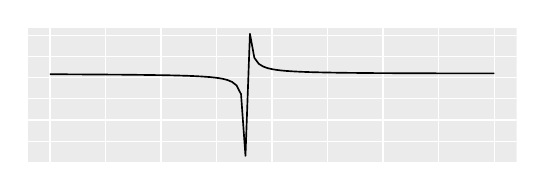
\begin{tikzpicture}[x=1pt,y=1pt]
            \begin{scope}
                \path[clip] ( 34.64, 18.22) rectangle (211.31, 66.77);
                \definecolor{fillColor}{gray}{0.92}
        
                \path[fill=fillColor] ( 34.64, 18.22) rectangle (211.31, 66.77);
                \definecolor{drawColor}{RGB}{255,255,255}
        
                \path[draw=drawColor,line width= 0.3pt,line join=round] ( 34.64, 25.82) --
                    (211.31, 25.82);
        
                \path[draw=drawColor,line width= 0.3pt,line join=round] ( 34.64, 41.08) --
                    (211.31, 41.08);
        
                \path[draw=drawColor,line width= 0.3pt,line join=round] ( 34.64, 56.34) --
                    (211.31, 56.34);
        
                \path[draw=drawColor,line width= 0.3pt,line join=round] ( 62.75, 18.22) --
                    ( 62.75, 66.77);
        
                \path[draw=drawColor,line width= 0.3pt,line join=round] (102.90, 18.22) --
                    (102.90, 66.77);
        
                \path[draw=drawColor,line width= 0.3pt,line join=round] (143.05, 18.22) --
                    (143.05, 66.77);
        
                \path[draw=drawColor,line width= 0.3pt,line join=round] (183.20, 18.22) --
                    (183.20, 66.77);
        
                \path[draw=drawColor,line width= 0.6pt,line join=round] ( 34.64, 33.45) --
                    (211.31, 33.45);
        
                \path[draw=drawColor,line width= 0.6pt,line join=round] ( 34.64, 48.71) --
                    (211.31, 48.71);
        
                \path[draw=drawColor,line width= 0.6pt,line join=round] ( 34.64, 63.97) --
                    (211.31, 63.97);
        
                \path[draw=drawColor,line width= 0.6pt,line join=round] ( 42.68, 18.22) --
                    ( 42.68, 66.77);
        
                \path[draw=drawColor,line width= 0.6pt,line join=round] ( 82.83, 18.22) --
                    ( 82.83, 66.77);
        
                \path[draw=drawColor,line width= 0.6pt,line join=round] (122.98, 18.22) --
                    (122.98, 66.77);
        
                \path[draw=drawColor,line width= 0.6pt,line join=round] (163.13, 18.22) --
                    (163.13, 66.77);
        
                \path[draw=drawColor,line width= 0.6pt,line join=round] (203.28, 18.22) --
                    (203.28, 66.77);
                \definecolor{drawColor}{RGB}{0,0,0}
        
                \path[draw=drawColor,line width= 0.6pt,line join=round] ( 42.68, 49.93) --
                    ( 44.28, 49.93) --
                    ( 45.89, 49.92) --
                    ( 47.49, 49.91) --
                    ( 49.10, 49.91) --
                    ( 50.71, 49.90) --
                    ( 52.31, 49.89) --
                    ( 53.92, 49.88) --
                    ( 55.52, 49.87) --
                    ( 57.13, 49.87) --
                    ( 58.74, 49.86) --
                    ( 60.34, 49.85) --
                    ( 61.95, 49.84) --
                    ( 63.55, 49.82) --
                    ( 65.16, 49.81) --
                    ( 66.77, 49.80) --
                    ( 68.37, 49.79) --
                    ( 69.98, 49.77) --
                    ( 71.58, 49.76) --
                    ( 73.19, 49.74) --
                    ( 74.80, 49.72) --
                    ( 76.40, 49.70) --
                    ( 78.01, 49.68) --
                    ( 79.61, 49.66) --
                    ( 81.22, 49.63) --
                    ( 82.83, 49.61) --
                    ( 84.43, 49.58) --
                    ( 86.04, 49.55) --
                    ( 87.64, 49.51) --
                    ( 89.25, 49.47) --
                    ( 90.86, 49.42) --
                    ( 92.46, 49.37) --
                    ( 94.07, 49.31) --
                    ( 95.67, 49.23) --
                    ( 97.28, 49.15) --
                    ( 98.89, 49.04) --
                    (100.49, 48.92) --
                    (102.10, 48.75) --
                    (103.70, 48.54) --
                    (105.31, 48.25) --
                    (106.92, 47.83) --
                    (108.52, 47.15) --
                    (110.13, 45.89) --
                    (111.74, 42.74) --
                    (113.34, 20.43) --
                    (114.95, 64.56) --
                    (116.55, 55.88) --
                    (118.16, 53.70) --
                    (119.77, 52.71) --
                    (121.37, 52.14) --
                    (122.98, 51.77) --
                    (124.58, 51.51) --
                    (126.19, 51.31) --
                    (127.80, 51.16) --
                    (129.40, 51.05) --
                    (131.01, 50.95) --
                    (132.61, 50.87) --
                    (134.22, 50.80) --
                    (135.83, 50.74) --
                    (137.43, 50.69) --
                    (139.04, 50.65) --
                    (140.64, 50.61) --
                    (142.25, 50.58) --
                    (143.86, 50.55) --
                    (145.46, 50.52) --
                    (147.07, 50.49) --
                    (148.67, 50.47) --
                    (150.28, 50.45) --
                    (151.89, 50.43) --
                    (153.49, 50.42) --
                    (155.10, 50.40) --
                    (156.70, 50.39) --
                    (158.31, 50.37) --
                    (159.92, 50.36) --
                    (161.52, 50.35) --
                    (163.13, 50.34) --
                    (164.73, 50.33) --
                    (166.34, 50.33) --
                    (167.95, 50.32) --
                    (169.55, 50.31) --
                    (171.16, 50.31) --
                    (172.76, 50.30) --
                    (174.37, 50.29) --
                    (175.98, 50.29) --
                    (177.58, 50.28) --
                    (179.19, 50.28) --
                    (180.80, 50.28) --
                    (182.40, 50.27) --
                    (184.01, 50.27) --
                    (185.61, 50.27) --
                    (187.22, 50.27) --
                    (188.83, 50.26) --
                    (190.43, 50.26) --
                    (192.04, 50.26) --
                    (193.64, 50.26) --
                    (195.25, 50.26) --
                    (196.86, 50.25) --
                    (198.46, 50.25) --
                    (200.07, 50.25) --
                    (201.67, 50.25) --
                    (203.28, 50.25);
            \end{scope}
        \end{tikzpicture}
    \end{center}
\end{example}

\begin{theorem}[Liouville 1841 \cite{吉田耕作-微分方程式}]
    斉次な$n$次のRiccati方程式で,係数が定数$p\equiv a,q\equiv b$の場合を考える.
    求積可能な場合は次に限る:
    \begin{enumerate}
        \item $n=0$または$a=0$または$b=0$ならば,変数分離型である.
        \item $n=-2$の場合,$z=1/y$についての斉次方程式になる.
        \item $n=-\frac{4m}{2m-1}\;(m\in\N^+)$の場合,$n=0$の場合と同様変数分離型に帰着される.
        \item $n=-\frac{4m}{2m+1}\;(m\in\N^+)$の場合,(3)の手続きを繰り返すことでやはり変数分離型に帰着する.
    \end{enumerate}
\end{theorem}

\section{変数係数線型NODE}

\begin{tcolorbox}[colframe=ForestGreen, colback=ForestGreen!10!white,breakable,colbacktitle=ForestGreen!40!white,coltitle=black,fonttitle=\bfseries\sffamily,
title=]
    変数係数の線型NODEについて
    \begin{enumerate}
        \item 変数係数の線型NODEについて,斉次化の基本解がわかれば,非斉次の場合も解ける(特解の公式\ref{thm-special-solution-to-linear-ODE}).
        よって,斉次な場合を考えれば十分である.
        \item Fuchs型の例であり,そしてその全てでもあるのがGaussの超幾何方程式である.
        直交多項式,Whittaker関数,Airy関数はいずれもこれ(の合流や特殊化)に属する.
        \item 一方で,Bessel方程式は$\infty$に不確定特異点を持ち,Fuchs型に入らない方程式の殆どを担う.
    \end{enumerate}
\end{tcolorbox}

\subsection{枠組み}

\begin{tcolorbox}[colframe=ForestGreen, colback=ForestGreen!10!white,breakable,colbacktitle=ForestGreen!40!white,coltitle=black,fonttitle=\bfseries\sffamily,
title=]
    理論の枠組みは次の通りである\cite{大島利雄-ODE}:
    \begin{enumerate}
        \item 係数が解析的ならば,最高階の係数の零点を除いて,局所的な解が一意に存在し,(多価)解析解に解析接続出来る.
        しかし多価解析解を考えるのであれば,$\R$上とするのではなく,係数は一般の有理型関数として$\wh{\C}$上の方程式と考える方が筋が良い.
        こうして解は$\wh{\C}$上に有限個の特異点を持つ多価解析関数=Riemann面上の関数になる.
        \item 特に確定特異点しか持たない方程式について,Fuchsの理論が立つ.
        それでも,特異点周りの局所的な知識を繋げる大域解析は困難である.
        不確定特異点は更に難しいが,Poincare, Birkoffらから始まる理論により,階数に等しいだけの独立な形式解を通じて,適当な扇形領域でその形式解に漸近展開される独立解を得ることが出来る.特異点の周りの状況は角領域での接続係数に当たるStokes係数で記述される.
    \end{enumerate}
    まず,変数係数線型ODEを複素領域上の方程式とみる.
    そして特に係数が有理型関数である場合を扱おう.
\end{tcolorbox}

\begin{problem}[有理型関数係数の常微分方程式]
    領域$D\osub\wh{C}$上の,有理型関数$a_1,\cdots,a_n\in H(D)$を係数に持つ線型ODE
    \[\text{(E')} \quad ,a_0(t)\dd{^ny}{x^n}+a_1(t)\dd{^{n-1}y}{x^{n-1}}+\cdots+a_{n-1}(t)\dd{y}{x}+a_n(t)y=0\quad a_0,\cdots,a_n\in H(D)\]
    を考える.あるいは同値なことだが,$p_i:=a_i/a_0\;(i\in[n])$として,最高次係数を1に正規化した場合の方程式
    \[\text{(E)} \quad \dd{^ny}{x^n}+p_1(t)\dd{^{n-1}y}{x^{n-1}}+\cdots+p_{n-1}(t)\dd{y}{x}+p_n(t)y=0,\quad p_1,\cdots,p_n\in H(D)\]
    を考える.
    \begin{enumerate}
        \item $a_0$の零点,すなわち,$p_1,\cdots,p_n$の特異点の合併を\textbf{特異点}という.ただし,$\infty\in\wh{\C}$は変換$t\mapsto\frac{1}{t}$により原点の特異性としてみて判断する.
        \item 特異点でない点,すなわち,$p_1,\cdots,p_n$のいずれも正則になる点を,方程式の\textbf{通常点}という.
        \item 特異点$a\in D$が\textbf{確定}(regular)であるとは,各$p_i\;(i\in[n])$が$a$を高々$i$位の極として持つことをいう.
    \end{enumerate}
\end{problem}

\begin{proposition}[確定特異点の特徴付け \cite{大島利雄-ODE}]
    $x=0\in\wh{\C}$について,次は同値:
    \begin{enumerate}
        \item (E')の確定特異点である.
        \item (E')の任意の解は,局所的に多項式増大である:$\exists_{m\in\N}\;\abs{x^mu(x)}<1\;(0<\abs{x}\ll1,\abs{\arg x}<2\pi)$.
        \item (E')の解がなす有理型関数上の加群$\F(\Delta(a,\ep))$が,一般化されたFrobenius級数$z^a(\log z)^b\;(a\in\C,b\in\N)$によって生成される\footnote{\url{https://ncatlab.org/nlab/show/regular+singular+point}}.
    \end{enumerate}
    この条件が成り立つとき,関数$\frac{x^{n-j}a_j(x)}{a_n(x)}$は$x=0$上にも正則に延長する.
    一般の点については,Mobius変換を通じて同様の消息が成り立つ.
\end{proposition}

\begin{theorem}[係数が正則である場合]\mbox{}
    \begin{enumerate}
        \item 一般に,正規型方程式$x'=f(t,x)$について,$f$が$(t_0,x_0)\in\C^2$近傍で正則ならば,$(t_0,x_0)$-初期値問題の一意な局所解は再び正則である.
        \item 方程式(E)について,$p_1,\cdots,p_n$が正則でもあるならば,解は$D$上正則である.
        \item 方程式(E)について,$p_1,\cdots,p_n$が正則でもあるとする.$x_1,\cdots,x_n$を任意の解とすると,そのWronskianは,$D$上のある一点で消えるならば$I$上で零であり,ある一点で非零ならば$I$上で消えない.
    \end{enumerate}
\end{theorem}

\begin{remarks}
    こうして,もし$p_i\in\O(D)$なら級数解として,$p_i$が確定特異点しか持たないならば,Frobenius級数$y(z)=(z-a)^r\sum_{n\in\N}c_n(z-a)^n$の形で解を探すことが方針となる.
    これをFrobeniusの方法という.
    そして大域解は,各関数の芽を解析接続して得る必ずしも一価とは限らない多価解析関数として得られる.
\end{remarks}

\begin{theorem}
    方程式(E)について,
    \begin{enumerate}
        \item $a\in D$は通常点であるとする.この特異点を含まない近傍での局所解の全体$\F(\Delta(a,\ep))$は$n$次元の複素線型空間である.
    \end{enumerate}
\end{theorem}

\subsection{Fuchs型}

\begin{tcolorbox}[colframe=ForestGreen, colback=ForestGreen!10!white,breakable,colbacktitle=ForestGreen!40!white,coltitle=black,fonttitle=\bfseries\sffamily,
title=]
    Fuchs型の方程式は確定特異点のみを持つから,
    \begin{enumerate}
        \item Frobenius級数の方法は一般的な形で通用する.
        \item さらに,局所的な解は有限次元線型空間をなし,特異点の近傍でh多項式増大度しか持たない.
        逆にこのような$\wh{\C}$上の多価解析関数Fuchs型方程式の解である.
    \end{enumerate}
\end{tcolorbox}

\begin{problem}
    $D\osub\C$上で確定特異点しか持たない線型ODE
    \[\text{(FE)}\quad \dd{^ny}{x^n}+p_1(t)\dd{^{n-1}y}{x^{n-1}}+\cdots+p_{n-1}(t)\dd{y}{x}+p_n(t)y=0\]
    を\textbf{Fuchs型}という.
\end{problem}

\begin{theorem}[Fuchs]\mbox{}
    \begin{enumerate}
        \item (Fuchs criterium) Fuchs型の方程式は正則な特異点しか持たない.
        \item $n=2$とし,$a\in D$を確定特異点とする.最も近いほかの特異点までの距離を$R$とする.
        任意の基本解$y_1,y_2$は,円環領域$\Delta^*(a,R)$上で正則で,
        次いずれかの形で表せる:
        \[\begin{cases}
            y_1(z)=(z-a)^{\rho_1}\sum_{n\in\N}c_n(z-a)^n\\
            y_2(z)=(z-a)^{\rho_2}\sum_{n\in\N}d_n(z-a)^n
        \end{cases}\qquad\rho_1,\rho_2\in\C,c_0d_0\ne0.\]
        \[\begin{cases}
            y_1(z)=(z-a)^{\rho_1}\sum_{n\in\N}c_n(z-a)^n\\
            y_2(z)=(z-a)^{\rho_2}\sum_{n\in\N}d_n(z-a)^n+Ay_1(z)\log(z-a)
        \end{cases}\qquad\rho_1,\rho_2,A\in\C,c_0d_0\ne0.\]
    \end{enumerate}
\end{theorem}
\begin{remarks}
    特異点が確定特異点とは限らず,一般の孤立特異点とすると,(2)に同様な結果が$\sum_{n\in\Z}$として示せる.
    実はこの性質は確定特異点を特徴付ける.
\end{remarks}

\begin{corollary}[より簡単な表現]
    $t=0$に確定特異点を持つ2階の線型方程式
    \[x''+\frac{p(t)}{t}x'+\frac{q(t)}{t^2}x=0\]
    の決定方程式$\lambda(\lambda-1)+p(0)\lambda+q(0)=0$の2解を$\rho_1,\rho_2$とし,$t=0$の近傍で解析的で$u_1(0)\ne0,u_2(0)\ne0\;(N\ne0\text{のとき})$を満たすとする.
    解は
    \begin{enumerate}
        \item $\rho_1-\rho_2\notin\Z$のとき,$x_1(t)=t^{\rho_1}u_1(t),x_2(t)=t^{\rho_2}u_2(t)$.
        \item $\rho_1-\rho_2\in\N$のとき,$x_1(t)=t^{\rho_1}u_1(t),x_2(t)=cx_1(t)\log t+t^{\rho_2}u_2(t)$.
    \end{enumerate}
    と表せる.逆に,この2つの解を持つ2階線型方程式の係数は,$t=0$で解析的な関数$p,q$を用いて$p(t)/t,q(t)/t^2$の形である必要がある.
\end{corollary}

\subsection{Eulerの微分方程式}

\begin{tcolorbox}[colframe=ForestGreen, colback=ForestGreen!10!white,breakable,colbacktitle=ForestGreen!40!white,coltitle=black,fonttitle=\bfseries\sffamily,
title=]
    変数係数線型ODEのうち,可解なものの一つに,係数が導関数の位数と同じものがある:$p_i(x)=a_ix^{n-i}$.
    これがFuchs理論の雛形となる.
\end{tcolorbox}

\begin{problem}
    所与の区分的$C^1$-級な非線形項$q$について,$n$次の\textbf{Cauchy-Euler方程式}とは,
    \[a_nt^nx^{(n)}+a_{n-1}t^{n-1}x^{(n-1)}+\cdots+a_0x=q(t),\quad a_n,\cdots,a_0\in\R,q\in PC^1(\R)\]
    をいう.特に,$n=2$の場合
    \[t^2x''+atx'+bx=q(t),\qquad a,b\in\R,q\in PC^1(\R).\]
    を考える.
\end{problem}

\begin{proposition}
    $n=2$の斉次Euler方程式
    \[t^2x''+atx'+bx=0\]
    の解$x$は,$y(\tau):=x(e^\tau)$について,
    \[y''+(a-1)y'+by=0\]
    を満たす.
    すなわち,
    特性方程式
    \[\lambda(\lambda-1)+a\lambda+b=0\]
    の
    \begin{enumerate}
        \item 相異なる2解$\lambda_1,\lambda_2$について,
        \[x(t)=C_1t^{\lambda_1}+C_2t^{\lambda_2},\quad C_1,C_2\in\R.\]
        \item 重根$\lambda_1$について,
        \[x(t)=C_1t^{\lambda_1}+C_2t^\lambda\log t,\quad C_1,C_2\in\R.\]
        \item 相異なる2つの複素根$\sigma\pm i\mu$について,
        \[x(t)=C_1t^\sigma\cos(\mu\log t)+C_2t^\sigma(\mu\log t),\quad C_1,C_2\in\R.\]
    \end{enumerate}
\end{proposition}
\begin{Proof}
    変数変換$t=e^\tau$を施すと,$y(\tau):=x(e^\tau)$についての方程式
    \[y''+(a-1)y'+by=0\]
    に変換される.よって,特性方程式
    \[\lambda(\lambda-1)+a\lambda+b=0\]
    の2解$\lambda_1,\lambda_2$を用いて,$y$の基本解が求まる.
\end{Proof}

\begin{definition}\mbox{}
    \begin{enumerate}
        \item Euler方程式に付随する線型方程式の特性方程式を\textbf{決定方程式}という.
        \item 特に(1)の場合,初期条件$x(0)=0$を与えても定数$C_1,C_2\in\R$が決定できない.この点を\textbf{特異点}という.一方で,$t>0$において初期条件を与えたらこのようなことは起こらない.
    \end{enumerate}
\end{definition}

\begin{example}
    \[t^2x''-tx'-3x=\log t\]
    を考える.
    \begin{enumerate}
        \item 付随する$y(s):=x(e^s)$に関する線型方程式
        \[y''-2y'-3y=s\]
        の基本解は$e^{-s},e^{3s}$より,Wronskianは
        \[W(s)=\begin{vmatrix}
            e^{3s}&e^{-s}\\3e^{3s}&-e^{-s}
        \end{vmatrix}=-4e^{2s}.\]
        \item よって,特解の基本解による公式\ref{thm-special-solution-to-linear-ODE}より,
        \[\eta(s)=-\frac{s}{3}+\frac{2}{9}+\frac{e^s}{36}-\frac{e^{-s}}{4}.\]
        が見つかる.特に,元の方程式の特解として
        \[\eta(t)=-\frac{1}{3}\log t+\frac{2}{9}\]
        が見つかる.
        \item 以上より,
        \[x(t)=C_1t^3+C_2t^{-1}-\frac{1}{3}\log +\frac{2}{9}.\]
    \end{enumerate}
\end{example}

\subsection{Gaussの微分方程式}

\begin{tcolorbox}[colframe=ForestGreen, colback=ForestGreen!10!white,breakable,colbacktitle=ForestGreen!40!white,coltitle=black,fonttitle=\bfseries\sffamily,
title=]
    
\end{tcolorbox}

\begin{problem}[hypergeometric differential equation]
    \[\text{(GE)}\quad t(1-t)x''+(\gamma-(\al+\beta+1)z)x'-\al\beta x=0,\qquad\al,\beta,\gamma\in\C.\]
    を\textbf{Gaussの超幾何微分方程式}という.
    特異点は$\{0,1,\infty\}\subset\wh{\C}$に持つ.
    \begin{enumerate}
        \item $U\osub\wh{\C}\setminus\{0,1,\infty\}$を領域,$\F(U)$を$U$上の正則解全体とする.
        \item $(\al)_n:=\al(\al+1)\cdots(\al+n-1)=\frac{\Gamma(\al+n)}{\gamma(\al)}$とする.これをPochhammer記号という.
        \item 次の冪級数が収束するならば,これが定める$\Delta$上の関数を\textbf{Gaussの超幾何関数}という:
        \[F(\al,\beta,\gamma;x):=\sum_{n\in\N}\frac{(\al)_n(\beta)_n}{(\gamma)_nn!}x^n,\quad\abs{x}<1,\al,\beta,\gamma\in\C.\]
        例えば,$\gamma$が負整数のとき,定義されない.
    \end{enumerate}
    存在するならば,これは方程式(GE)の解になっていることが分かる.
    Gaussの超幾何関数は解析接続によって大域的な性質がよく分かる稀有な関数である.
\end{problem}

\begin{proposition}[Gauss summation formula]\mbox{}
    \begin{enumerate}
        \item $0<\Re\beta<\Re\gamma,0<\arg(x-1)<2\pi$において,次の積分表示を持つ:
        \[F(\al,\beta,\gamma;x)=\frac{\Gamma(\gamma)}{\Gamma(\beta)\Gamma(\gamma-\beta)}\int^1_0t^{\beta-1}(1-t)^{\gamma-\beta-1}(1-tx)^{-\al}dt.\]
        \item 特に,$\Re(\gamma-\beta-\al)>0$のとき,$x=1$とすれば,右辺の積分はBeta関数となり,このとき
        \[F(\al,\beta,\gamma;1)=\frac{\Gamma(\gamma)}{\Gamma(\beta)\Gamma(\gamma-\beta)}\frac{\Gamma(\beta)\Gamma(\gamma-\al-\beta)}{\Gamma(\gamma-\al)}\]
        よって,
        \[C_{\al,\beta,\gamma}:=F(\al,\beta,\gamma;1)=\frac{\Gamma(\gamma)\Gamma(\gamma-\al-\beta)}{\Gamma(\gamma-\al)\Gamma(\gamma-\beta)}.\]
        さらに,$\Re\al+\Re\beta<\Re\gamma$ならば,左辺の級数は絶対収束する.
    \end{enumerate}
\end{proposition}
\begin{remark}
    (1)の積分表示も,
    \[(1-tx)^{-\al}=\sum_{n\in\N}\frac{(\al)_n}{n!}t^nx^n\]
    として,$x^n$の係数を見ると,各項の積分がBeta関数になり,
    \[\frac{\Gamma(\gamma)}{\Gamma(\beta)\Gamma(\gamma-\beta)}\frac{(\al)_n}{n!}\frac{\Gamma(\beta+n)\Gamma(\gamma-\beta)}{\Gamma(\gamma+n)}=\frac{(\al)_n(\beta)_n}{(\gamma)_nn!}\]
    を得るため,等式の成立がわかる.
\end{remark}

\begin{proposition}[Riemann]
    $F(\al,\beta,\gamma;x)$はGaussの超幾何微分方程式の解であり,原点で正則でかつ$1$の値を取る解はこれに限る.
\end{proposition}

\begin{history}
    岩波全書の公式集「特殊関数」の7割以上がGaussの超幾何関数が占める.
    いわば,「一番わかる」関数であり,Bessel関数,Legendre多項式,Whittaker関数などがこれに属する.
    残りの2割強がGamma関数や楕円函数など,Gaussの超幾何関数との関連によりわかっている関数で,残りが楕円体関数となる.
\end{history}

\begin{theorem}
    方程式(GE)について,
    \begin{enumerate}
        \item 任意の領域$U\osub\wh{\C}\setminus\{0,1,\infty\}$について,$\F(U)$は2次元の複素線型空間となる.
        \item 任意の部分領域$U'\osub U$について,$\F(U)|_{U'}=\F(U')$.
        \item ある$\varphi_1,\varphi_2\in\O(U)$について,$\F(U)=\C\varphi_1+\C\varphi_2$が成り立つとする.このとき,ある定数$C\in\R^+,N\in\N$が存在して,
        \[\abs{\varphi_j(x)}\le C\abs{x}^{-N}\quad(j\in[2],x\in U,\abs{\arg x}<2\pi,\abs{x}<1/2).\]
        特に,(GE)はFuchs型である(確定特異点しかもたない).
        \item $\psi_1(0)=\psi_2(0)=1$を満たす$U\cup\{0\}$上で正則な関数$\psi_1,\psi_2$が存在して,
        \[\F(U)=\C x^0\psi_1(x)+\C x^{1-\gamma}\psi_2(x)\]
        と表せる.特に,$x=0$での特性指数は$\{0,1-\gamma\}\subset\C$である.
        さらに,$\psi_1(x)=F(\al,\beta,\gamma;x)$である.
        \item 同様にして,$x=1$での特性指数は$\{0,\gamma-\al-\beta\}$,$x=\infty$では$\{\al,\beta\}$である.
    \end{enumerate}
\end{theorem}
\begin{remarks}[方程式の特異点での局所的性質による統制]
    さらにRiemannによると,この$\{0,1,\infty\}$を確定特異点に持ち,それぞれの特性指数として上述のものを持つものは,Gaussの超幾何微分方程式を一意に定めていることを示した.
    実は,特異点が$\wh{\C}$上に3点しかなく,解析接続の線型和が2次元になる多価解析関数で既約なものがGaussの超幾何方程式に帰着する\cite{大島利雄-ODE}.
    そもそも,$\wh{\C}$上に特異点を持たない方程式は$u'=0$に限り,これはLiouvilleの定理に当たる.
    特異点が$\infty$のみで確定でもあるならば,方程式は$u^{(n)}=0$に限り,これは多項式になる.
\end{remarks}

\subsection{Legendreの多項式}

\begin{problem}
    \[((1-t^2)x')'+n(n+1)x=0,\qquad n\in\C\]
    というStrum-Liouville型の線型ODEをLegebdreの微分方程式という.
    この解をLegendreの陪関数といい,特に
    $n\in\N$のときの解は$n$次多項式$P_n$になり,これを\textbf{Legendreの多項式}という.
    \begin{enumerate}
        \item $\al=n+1,\beta=-n,\gamma=-1$としたGaussの微分方程式を$x:=\frac{1-x}{2}$について表した方程式に等しい.
        特に,確定特異点を$\{\pm1,\infty\}$に持つ.
        \item 次のようにしてStrum-Liouville型に変形される:
        \[((1-t^2)x)'=-\lambda x.\]
        \item $[-1,1]$上で正則な解を持つ(特に$\pm1$でも正則である)のは$l\in\N$の場合に限り,さらに$P_n(1)=1$を初期条件に課すと一意に定まる.
        この解は$L^2([-1,1],dx)$の直交基底をなす:
        \[\int^1_{-1}P_kP_ldx=\frac{2}{2l+1}\delta_{k,l}\]
    \end{enumerate}
\end{problem}
\begin{remark}
    一般化されたLegendre方程式
    \[(1-x^2)\dd{^2}{x^2}P^m_l(x)-2x\dd{}{x}P^m_l(x)+\paren{l(l+1)-\frac{m^2}{1-x^2}}P^m_l(x)=0,\quad m\le l\in\N.\]
    の解を\textbf{Legendreの陪多項式}という.
    なお,$m,l\in\Z$が$m\le l\in\N$を満たすことは,$[-1,1]$上で正則な解を持つことに同値.
\end{remark}

\begin{proposition}\mbox{}
    \begin{enumerate}
        \item (Rodrigues)
        \[P_n(t)=\frac{1}{2^nn!}\dd{^n}{x^n}((x^2-1)^n).\]
        特に,$n$の偶奇と$P_n$の偶奇は一致する:$P_n(-x)=(-1)^nP_n(x)$.
        \item (Bonnet)
        \[(n+1)P_{n+1}=(2n+1)tP_n(t)-nP_{n-1}(t).\]
        \item 母関数は
        \[S(t)=\frac{1}{\sqrt{1-2xt+t^2}}=\sum_{n\in\N}P_n(t)x^n.\]
    \end{enumerate}
\end{proposition}
\begin{remark}
    そもそもLegendreはNewtonian potential
    \[\frac{1}{\x-\x'}=\frac{1}{\sqrt{r^2+r'^2-2rr'\cos\gamma}}=\sum_{n\in\N}\frac{r'^l}{r^{l+1}}P_l(\cos\gamma).\]
    の展開係数として定義した.
\end{remark}

\subsection{Jacobi多項式}

\begin{tcolorbox}[colframe=ForestGreen, colback=ForestGreen!10!white,breakable,colbacktitle=ForestGreen!40!white,coltitle=black,fonttitle=\bfseries\sffamily,
title=]
    Legendreの多項式を一般化する形で,$L^2([-1,1])$上の直交多項式系の殆ど(Gegenbauer多項式,Chebyshev多項式)を含むクラスである.
\end{tcolorbox}

\begin{problem}
    \[(1-t^2)x''+(\beta-\al-(\al+\beta+2)t)x'+n(n+\al+\beta+1)x=0,\qquad\al,\beta\in\C\]
    をJacobiの方程式という.$\al=\beta=0$のとき,Legendreの方程式である.
\end{problem}

\begin{definition}
    \[P_n^{(\al,\beta)}(t):=\frac{(\al+1)_n}{n!}{}_2F_1\paren{-n,1+\al+\beta+n,\al+1;\frac{1-t}{2}}=\frac{\Gamma(\al+n+1)}{n!\Gamma(\al+\beta+n+1)}\sum_{m=0}^n\comb{n}{m}\frac{\Gamma(\al+\beta+n+m+1)}{\Gamma(\al+m+1)}\paren{\frac{t-1}{2}}^m.\]
\end{definition}

\begin{proposition}
    \begin{enumerate}
        \item $L^2([-1,1],(1-x)^\al(1+x)^\beta dx)$の直交系をなす:
        \[\dint^1_{-1}P_n^{(\al,\beta)}P_m^{(\al,\beta)}dx=\frac{2^{\al+\beta+1}}{2n+\al+\beta+1}\frac{\Gamma(n+\al+1)\Gamma(n+\beta+1)}{\Gamma(n+\al+\beta+1)n!}\delta_{n,m},\qquad\al,\beta>-1.\]
    \end{enumerate}
\end{proposition}

\subsection{Besselの微分方程式}

\begin{tcolorbox}[colframe=ForestGreen, colback=ForestGreen!10!white,breakable,colbacktitle=ForestGreen!40!white,coltitle=black,fonttitle=\bfseries\sffamily,
title=]
    BesselがKeplerの力学系を解析的に解く研究の中で定義した.
    Besselの方程式は$\infty$を(正則だが)不確定な特異点とする.
\end{tcolorbox}

\begin{problem}\label{prob-Bessel-eq}
    \[t^2x''+tx'+(t^2-\nu^2)x=0,\qquad\nu\in\C.\]
    を\textbf{Besselの方程式}という.
    \begin{enumerate}
        \item $\al\in\Z$のときの解を\textbf{円筒関数}という.円筒座標に関するLaplace方程式に現れるためである.
        \item $\al$が半整数であるとき,解を\textbf{Bessel球関数}という.球座標に関するHelmholtz方程式に現れるためである.
    \end{enumerate}
\end{problem}

\begin{proposition}[Bessel関数]
    \textbf{位数$\nu$の(第一種)Bessel関数}
    \[J_\nu(x):=\sum_{k\in\N}\frac{(-1)^k}{k!\Gamma(k+\nu+1)}\paren{\frac{x}{2}}^{2k+\nu},\qquad\nu\in\C\]
    について,
    \begin{enumerate}
        \item Bessel方程式の解である.
        \item 収束性と極限の性質
        \begin{enumerate}
            \item $x\ne0$のとき,または$x=0$かつ$\nu=0\lor\Re(\nu)=0$のとき,右辺は絶対収束する.
            $x>0\land\nu\in\R$のとき,$J_\nu$は実関数であることに注意.
            \item $x=0$近傍での振る舞いは,$\Re(\nu)>0$のとき,$\lim_{x\to0}J_\nu=0$.$\Re(\nu)<0\land\nu\notin\Z$のとき,$\lim_{x\to0}J_\nu=\infty$.
        \end{enumerate}
        \item $\nu\notin\Z$のとき,$J_\nu$は$\C\setminus(-\infty,0]$上の正則関数,$\C$上の多価関数を定め,一価にするには$(x/2)^\nu$の分枝を取る必要がある.
        \item $\nu\in\Z$のとき,$J_\nu$は整関数を定める.
        \item $\nu=:n\in\N$のとき,
        \[J_n(x)=\sum_{k\in\N}\frac{(-1)^k}{k!(n+k)!}\paren{\frac{x}{2}}^{2k+n},\quad J_{-n}(x)=(-1)^nJ_n(x).\]
        と表せる.
        特に,このとき$J_n,J_{-n}$は線型従属である.一方で,$\nu\notin\Z$のときは$J_\nu,J_{-\nu}$は線形独立になる.
    \end{enumerate}
    そこで,$n\in\N$の際に$J_n$と線形独立な,有用な解を見つける必要がある.
\end{proposition}

\begin{proposition}[Weber関数]
    \textbf{位数$\nu$の第二種Bessel関数}またはWeber関数
    \[Y_\nu(x):=\frac{\cos(\nu\pi)J_\nu(x)-J_{-\nu}(x)}{\sin(\nu\pi)},\qquad\nu\notin\Z.\]
    について,
    \begin{enumerate}
        \item $\nu\in\Z$の場合にも連続拡張すれば,任意の$\nu\in\C$についてBessel関数の解になる.
        \item $\nu=:n\in\Z$のとき,
        \begin{align*}
            Y_n(x)&\approx-\frac{(n-1)!}{\pi}\paren{\frac{x}{2}}^{-n}\quad x\to0,n\in\N^+,\\
            Y_0(x)&\approx\frac{2}{\pi}\log\frac{x}{2}\quad x\to0.
        \end{align*}
        \item 任意の$\nu\in\C$について$J_\nu,Y_\nu$は線型独立である.
    \end{enumerate}
\end{proposition}

\begin{remarks}
    $x\to0$において,$J_n$は$0$に収束し,特に有界だが,$Y_n$は発散する.
    Bessel関数に線形独立な解の他の取り方は当然無数に存在するが,Weber関数の重要性は$x\to\infty$の際の挙動に因る.
    Bessel関数が殆どcosならば,Weber関数は殆どsinになる.
\end{remarks}

\begin{proposition}[Bessel球関数の性質]
    $\nu-1/2\in\Z$ならば,
    \[J_\nu(x)=x^{-1/2}\paren{P_\nu(x)\cos x+Q_\nu(x)\sin x},\qquad P_\nu,Q_\nu\in\C(x).\]
    また,$J_\nu$が初等関数で表せるならば,$\nu-1/2\in\Z$である.
\end{proposition}
\begin{remarks}
    Bessel球関数とWeber球関数は,3次元自由粒子・井戸型ポテンシャルのSchrödinger方程式の動径方向の解を与える.
\end{remarks}

\subsection{Bessel関数の性質}

\begin{tcolorbox}[colframe=ForestGreen, colback=ForestGreen!10!white,breakable,colbacktitle=ForestGreen!40!white,coltitle=black,fonttitle=\bfseries\sffamily,
title=]
    Bessel関数のFourier係数としての特徴付けから積分表現を得る.ここから,$x\to\infty$での挙動を調べる手がかりを得る.
\end{tcolorbox}

\begin{proposition}[Bessel関数のFourier係数としての特徴付け]\mbox{}
    \begin{enumerate}
        \item 任意の$x,\nu\in\C$について,
        \[\dd{}{x}\paren{x^{-\nu}J_\nu(x)}=-x^{-\nu}J_{\nu+1}(x).\]
        \[xJ_{\nu-1}+xJ_{\nu+1}=2\nu J_\nu.\]
        \item 母関数:任意の$x\in\C$と$z\ne0$について,
        \[S(x,z):=\exp\paren{\frac{x}{2}\paren{z-\frac{1}{z}}}=\sum_{n\in\Z}J_n(x)z^n.\]
        特に,
        \[e^{ix\sin\theta}=\sum_{n\in\Z}J_n(x)e^{in\theta}.\]
        \item Besselの積分公式:
        \[J_n(x)=\frac{1}{\pi}\int^\pi_0\cos(nt-x\sin t)dt=\frac{1}{2\pi}\int^\pi_{-\pi}e^{i(nt-x\sin t)}dt.\]
        特に,
        \[J_n(x)=\begin{cases}
            \frac{2}{\pi}\int^{\pi/2}_0\cos(x\sin\theta)\cos n\theta d\theta&n\text{は偶数},\\
            \frac{2}{\pi}\int^{\pi/2}_0\sin(x\sin\theta)\sin n\theta d\theta&n\text{は奇数}.
        \end{cases}\]
    \end{enumerate}
\end{proposition}

\begin{theorem}[漸近挙動]
    任意の$\nu\in\R$について定数$C$が存在して,任意の$x\ge1$について,
    \[J_\nu(x)=\sqrt{\frac{2}{\pi x}}\cos\paren{x-\frac{\nu\pi}{2}-\frac{\pi}{4}}+E_\nu(x),\qquad \abs{E_\nu(x)}\le\frac{C}{x^{3/2}}.\]
\end{theorem}
\begin{remarks}
    証明はLaplace変換を用いるが,直感的には次の通り.Bessel関数の解$f(x)$に対して$g(x)=x^{1/2}f(x)$と変換すると,方程式は
    \[g''(x)+g(x)+\frac{1/4-\nu^2}{x^2}g(x)=0\]
    に変換される.よって$\abs{x}$が十分大きなとき,$g(x)\approx a\cos(x+b),a\sin(x+b)$の形をしていることが予想出来る.
\end{remarks}

\begin{corollary}
    まず$\nu\notin\Z$のとき,続いて$\nu\in\Z$のときも,次が成り立つ:
    \[Y_\nu(x)\approx\sqrt{\frac{2}{\pi x}}\sin\paren{x-\frac{\nu\pi}{2}-\frac{\pi}{4}}+O(\abs{x}^{-3/2}),\qquad (\abs{x}\to\infty).\]
\end{corollary}

\begin{theorem}[Bessel関数と特異なSturm-Liouville理論]
    $\nu\ge0,b>0$とする.
    \begin{enumerate}
        \item $\{\lambda_k\}\subset\R_+$を$J_\nu$の正な零点,$\phi_k(x):=J_\nu(\lambda_kx/b)$とする.
        このとき,$(\phi_k)$は$L^2([0,b])$の直交基底であり,
        \[\norm{\phi_k}^2_{L^2([0,b])}=\frac{b^2}{2}J_{\nu+1}(\lambda_k)^2.\]
        \item $c\ge-\nu$とする.$\{\wt{\lambda}_k\}\subset\R_+$を$cJ_\nu(x)+xJ'_\nu(x)$の正な零点,$\psi_k(x):=J_\nu(\wt{\lambda}_kx/b)$とする.
        \begin{enumerate}
            \item $c>-\nu$のとき,$(\psi_k)$は$L^2([0,b])$の直交基底である.
            \item $c=\nu$のとき,$(\psi_k)$は$\psi_0(x):=x^\nu$と併せれば直交基底である.
            このとき,
        \[\norm{\psi_k}^2=\frac{b^2(\lambda^2_k-\nu^2+c^2)}{2\lambda_k^2}J_\nu(\lambda_k)^2,\quad(k\ge1),\quad\norm{\psi_0}^2=\frac{b^{2\nu +2}}{2\nu+2}.\]
        \end{enumerate}
    \end{enumerate}
\end{theorem}
\begin{remarks}
    重み関数が$\id_\R$となるのが肝要である.(1), (2)を用いた展開をFourier-Bessel級数といい,特に(2)に基づくものを\textbf{Dini級数}という.
\end{remarks}

\subsection{Hankel関数}

\begin{definition}
    \[H_\nu^{(1)}(x):=J_\nu(x)+iY_\nu(x),\quad H_\nu^{(2)}(x):=J_\nu(x)-iY_\nu(x).\]
    をそれぞれ第一・第二\textbf{Hankel関数},または,第三種Bessel関数という.
\end{definition}

\begin{problem}\mbox{}
    \begin{enumerate}
        \item $x$の係数の$t^2$の符号を負にしたもの
        \[t^2x''+tx'-(t^2+\nu^2)x=0,\qquad\nu\in\C.\]
        を\textbf{修正Bessel方程式}という.
        \item  $x$の係数の$t^2$を$\mu^2t^2$としたもの
        \[t^2x''+tx'+(\mu^2t^2-\nu^2)x=0,\qquad\nu\in\C.\]
        を\textbf{一般化Bessel方程式}という.
    \end{enumerate}
\end{problem}

\begin{proposition}\mbox{}
    \begin{enumerate}
        \item \textbf{修正Bessel関数}
        \[I_\nu(x):=i^{-\nu}J_\nu(ix)\]
        は修正Bessel方程式の解である.
        \item $\nu\notin\Z$のとき,$I_{-\nu},Y_\nu(ix)$は線形独立な解である.
        \item 修正Bessel関数
        \[K_\nu(x)=\frac{\pi}{2}\frac{I_{-\nu}(x)-I_\nu(x)}{\sin\nu\pi}\]
        は修正Bessel関数の解であり,任意の$\nu\in\C$について$I_\nu$と線形独立である.
    \end{enumerate}
\end{proposition}
\begin{remark}
    $J_\nu(ix)$も解であるが,$x,\nu\in\R$の際に実関数になるように調整したものである.
\end{remark}

\subsection{2階線型方程式の標準形}

\begin{tcolorbox}[colframe=ForestGreen, colback=ForestGreen!10!white,breakable,colbacktitle=ForestGreen!40!white,coltitle=black,fonttitle=\bfseries\sffamily,
title=]
    係数が変化する場合,一般に初等解法はない.
    次のような理論はある:
    \begin{enumerate}
        \item Bessel方程式に帰着できる形.
        \item 任意の2階線型方程式はStrum-Liouville型に変形できる.
        特に固有値問題に関連が深い型であり,
        従って多くの正規直交基底となる多項式系を定義する.
        \item Floquet理論.
    \end{enumerate}
\end{tcolorbox}

\begin{problem}
    \[-(p(t)x')'+q(t)x=\lambda w(x)x,\qquad p,w>0,p,p',q,w\in C([a,b]).\]
    の形の2階の線型微分方程式を\textbf{Strum-Liouville型}という.
    これに,境界値問題
    \[\text{(SL-B)}\quad \al_1x_1(a)+\al_2x_2(a)=0\;(\al_1^2+\al_2^2>0),\quad\beta_1x_1(b)+\beta_2x_2(b)=0\;(\beta_1^2+\beta_2^2>0).\]
    \begin{enumerate}
        \item これは
        \[-p(t)x''-p'(t)x'+(q(t)-\lambda w(x))x=\underbrace{\paren{-p(t)\dd{^2}{t^2}-p'(t)\dd{}{t}+(q(t)-\lambda w(x))}}_{=:L}x=0\]
        に等しい.$L$を\textbf{Strum-Liouville形式}という.
        \item 零関数はこの解である.これ以外の解を非自明な解と言い,そのときの$\lambda$を固有値,解を\textbf{固有関数}という.$w$を\textbf{重み関数}という.
        \item 任意の2階線型方程式$x''+a(t)x'+b(t)x=0$は,両辺に$p(t)=\exp\paren{\int a(t)dt}$を乗じることで,Strum-Liouville型$(p(t)x')'+q(t)x=0$に帰着する.
    \end{enumerate}
\end{problem}

%\begin{theorem}
%    $x''+a_1(t)x'+a_2(t)x=0$について,
%    \begin{enumerate}
%        \item $\int\exp\paren{-\int^ta_1(s)ds}dt=s$によって変数変換すると,標準形
%        \[\dd{^2x}{s^2}+\exp\paren{2\int^{t(s)}a_1(\tau)d\tau}a_2(t(s))x=0\]
%        に帰着する.特に,$a_2(t)=c\exp\paren{-2\int^ta_1(\tau)d\tau}$の関係があるとき,定数係数である.
%        \item $x=y\exp\paren{-\int^t\frac{1}{2}a_1(\tau)d\tau}$によって変数変換すると,標準形
%        \[y''+\paren{a_2(t)-\frac{1}{2}a'_1(t)-\frac{1}{4}a_1(t)^2}y=0\]
%        に帰着する.
%    \end{enumerate}
%\end{theorem}

\begin{theorem}
    方程式
    \[x^pf''(x)+px^{p-1}f'(x)+(ax^q+bx^{p-2})f(x)=0,\quad(1-p)^2-4b\ge0,q-p+2>0.\]
    について,
    \[\al:=\frac{1-p}{2},\quad\beta:=\frac{q-p+2}{2},\quad\lambda:=\frac{2\sqrt{\abs{a}}}{q-p+2},\quad\nu:=\frac{\sqrt{(1-p)^2-4b}}{q-p+2}.\]
    とする.
    \begin{enumerate}
        \item $a>0$のとき,一般解は
        \[f(x)=x^\al\paren{c_1J_\nu(\lambda x^\beta)+c_2Y_\nu(\lambda x^\beta)}.\]
        \item $a<0$のとき,一般解は
        \[f(x)=x^\al\paren{c_1I_\nu(\lambda x^\beta)+c_2K_\nu(\lambda x^\beta)}.\]
    \end{enumerate}
\end{theorem}

\subsection{Airy方程式}

\begin{problem}
    標準形の2階線型ODE
    \[x''-tx=0\]
    を\textbf{Airy方程式}またはStokes方程式という.
    \begin{enumerate}
        \item これは転回点(turning point: 方程式の解が振動型から指数型へ変わる特徴点)を持つ最も単純な2階線型ODEである.
        \item エアリー関数は三角ポテンシャル井戸に留め置かれた粒子に対する、あるいは一次元定力場における粒子に対するシュレーディンガー方程式の解である。
    \end{enumerate}
\end{problem}

\begin{proposition}[Bessel方程式への帰着]
    一般解は
    \[f(x)=x^{1/2}\paren{c_1I_{1/3}\paren{\frac{2}{3}x^{3/2}}+c_2K_{1/3}\paren{\frac{2}{3}x^{3/2}}}.\]
\end{proposition}

\begin{proposition}[級数法による解]
    \[x_1(t)=1+\sum_{m\in\N^+}\frac{1\cdot 4\cdot 7\cdots(3m-2)}{(3m)!}t^{3m},\quad x_2(t)=t+\sum_{m\in\N^+}\frac{2\cdot 5\cdot 8\cdots (3m-1)}{(3m+1)!}t^{3m+1}.\]
    はいずれもAiry方程式の解である整関数であり,互いに線型独立である.
\end{proposition}

\begin{proposition}\mbox{}
    \begin{enumerate}
        \item 広義積分
        \[A(t):=\frac{1}{\pi}\int^\infty_0\cos\paren{\frac{x^3}{3}+tx}dx\]
        は収束し,Airy方程式の解を定める.
        これは$\lim_{t\to\infty}A(t)=0$を満たす唯一の解である.
        \item 広義積分
        \[B(t):=\frac{1}{\pi}\int^\infty_0\paren{\exp\paren{-\frac{x^3}{3}+tx}+\sin\paren{\frac{x^3}{3}+tx}}dx\]
        も収束し,$t\to-\infty$において位相が$\pi/2$違う解を定める.
        \item $A,B$は解の基本系を定める.特にWronskianは$1/\pi$になる.
        \item Airy関数は直交性
        \[\int_\R A(x+t)A(x+s)dx=\delta(t-s)\]
        を持つ.
    \end{enumerate}
\end{proposition}

\section{2階線型ODEのStrum-Liouville理論}

\begin{tcolorbox}[colframe=ForestGreen, colback=ForestGreen!10!white,breakable,colbacktitle=ForestGreen!40!white,coltitle=black,fonttitle=\bfseries\sffamily,
title=]
    関数を特定の基底によってFourier展開する問題は自然界の各所に現れる.
    そこで,$L^2(\R)$またはその部分空間の基底を概観する.
\end{tcolorbox}

\begin{application}[spectral analysis]
    関数を周期関数からなる基底によってFourier展開し,各基底の係数の分布を見ることを\textbf{周波数分析}という.
    \begin{enumerate}
        \item 時系列変動の周期性を分析する際には,この周波数特性に注目することが最初のアイデアになる,これが1960s年代のCowles委員会の基本的発想である.
        \item 周波数特性が確率的になる場合,その密度関数を代わりに考え,これを\textbf{スペクトル密度}という.これが$1/f$に従うノイズを\textbf{ピンクノイズ}という.
        \begin{description}
            \item[生体] ニューロンの発火感覚,人の心拍の間隔,目の動き方,蛍の光り方
            \item[自然現象] 金属の抵抗
            \item[複雑現象] ろうそくの炎の揺れ方,電車の揺れ,小川のせせらぐ音,木漏れ日
        \end{description}
        この普遍性の結果,\textbf{$1/f$ゆらぎ}は人体に快適性を持つという研究があり,これを工業設計に応用することが考えられている.
        \item (粘性のある)流体の乱流中に生じる渦への外力は,大きいものから小さいものへと順に伝達される.これを\textbf{エネルギーカスケード}という.
        その名前は,周波数特性が滝のように高所から伝達していくことによる.
    \end{enumerate}
\end{application}

\subsection{Sturm-Liouville理論}

\begin{tcolorbox}[colframe=ForestGreen, colback=ForestGreen!10!white,breakable,colbacktitle=ForestGreen!40!white,coltitle=black,fonttitle=\bfseries\sffamily,
title=]
    自己随伴な線型作用素$L:L^2([a,b])\to L^2([a,b])$によって問題が$Lf=0$とかけるならば,スペクトル定理より,
    $Lf=0$の解によって$L^2([a,b])$の正規直交基底が取れることになる.
\end{tcolorbox}

\begin{problem}[formal self-adjoint \cite{Folland-Fourier}]
    $r:[a,b]\to\R$を消えない関数として,
    \[L(f):=rf''+qf'+pf,\qquad p,r,q\in C^2([a,b];\R)\]
    で定まる微分作用素$L:C^2([a,b])\to C([a,b])$を考える.
    $p,r,q$は実数値としたことに注意して,\textbf{形式的自己随伴}を
    \begin{align*}
        L^*(g)&=(rg)''-(qg)'+pg\\
        &=rg''+(2r'-q)g'+(r''-q'+p)g
    \end{align*}
    と定める.
\end{problem}

\begin{proposition}\mbox{}
    \begin{enumerate}
        \item $L$が形式的自己随伴作用素であることと,$q=r'$とは同値.
        \item (Lagrange's identity) 特に,$L$が形式的自己随伴作用素ならば,
        \[L(f)=rf''+r'f'+pf=(rf')'+pf\]
        と表せ,
        \[(L(f)|g)=(f|L(g))+\Square{r(f'\o{g}-f\o{g}')}^b_a\]
        が必要.
    \end{enumerate}
    特に,形式的自己随伴作用素$L$が実際に自己随伴になるかは,方程式$Lf=0$に課す境界条件に依る.
    適切な境界条件により$C^2([a,b])$の部分空間を取ることを考える.
\end{proposition}
\begin{Proof}
    まず$Lf$の第1項$rf''$について,部分積分より,
    \begin{align*}
        (rf''|g)=\int^b_a(rf'')\o{g}dx&=-\int^b_af'(r\o{g})dx+\Square{rf'\o{g}}^b_a\\
        &=\int^b_af(r\o{g})''dx+\Square{rf'\o{g}-f(r\o{g})'}^b_a.
    \end{align*}
    第2項の$qf'$は,
    \[(qf'|g)=\int^b_a(qf')\o{g}dx=-\int^b_af(q\o{g})'dx+\Square{qf\o{g}}^b_a.\]
    以上より,
    \[(L(f)|g)=(f|L^*(g))+\Square{r(f'\o{g}-f\o{g}')+(q-r')f\o{g}}^b_a.\]
    これと,$L$が形式的自己随伴であることより.
\end{Proof}

\begin{definition}[regular Sturm-Liouville problem]
    $[a,b]$上の\textbf{正則なSL問題}
    \[L(f)+\lambda wf=0,\quad B_1(f)=B_2(f)=0.\]
    とは,次の3つのデータが定める条件をいう:
    \begin{enumerate}
        \item $r>0,r',p\in C([a,b];\R)$が定める形式的自己随伴作用素$L(f):=(rf')'+pf$.
        \item 自己随伴的な境界条件.すなわち,
        \[\begin{cases}
            B_1(f)&=\al_1f(a)+\al_1'f'(a)+\beta_1f(b)+\beta_1'f'(b)=0,\\
            B_2(f)&=\al_2f(a)+\al_2'f'(a)+\beta_2f(b)+\beta_2'f'(b)=0.
        \end{cases}\quad(\al_i,\al_i',\beta_i,\beta_i'\in\R).\]
        であって,これを満たす$f,g\in C^2([a,b])$は
        \[\Square{r(f'\o{g}-f\o{g}')}^b_a=0\]
        も満たす.
        \item 重み関数$w\in C([a,b])_+$,
    \end{enumerate}
\end{definition}

\begin{theorem}
    正則なSL問題
    \[L(f)+\lambda wf=0,\quad B_1(f)=B_2(f)=0.\]
    について,
    \begin{enumerate}
        \item 任意の固有値は実数である.
        \item 違う固有値に属する固有関数は互いに直交する.
        \item 任意の固有空間は高々2次元である.
        \item 次の形をした境界条件(\textbf{分離型}という)については,固有空間は1次元である:
        \[\begin{cases}
            \al f(a)+\al'f'(a)=0,\\
            \beta f(b)+\beta'f'(b)=0
        \end{cases}\quad\al,\al',\beta,\beta'\in\R,(\al,\al')\ne(0,0),(\beta,\beta')\ne(0,0)\]
    \end{enumerate}
\end{theorem}

\begin{theorem}
    任意の正則なSL問題
    \[L(f)+\lambda wf=0,\quad B_1(f)=B_2(f)=0.\]
    について,
    \begin{enumerate}
        \item 固有関数のみからなる
        $L^2_w(a,b)$の正規直交基底$(\varphi_n)_{n\in\N}$が存在する.
        \item 対応する固有値の列を$\{\lambda_n\}\subset\R$とすると,$\lim_{n\to\infty}\lambda_n=\infty$.
        \item $f\in C^2([a,b])$が$B_1(f)=B_2(f)=0$を満たすならば,Fourier級数$\sum_{n=0}^N(f|\varphi_n)\varphi_n$は$f$に一様収束する.
    \end{enumerate}
\end{theorem}

\begin{theorem}[Strumの比較原理]
    2つのStrum-Liouville型$(p(t)x_1')'+q_1(t)x_1=0,(p(t)x_2')'+q_2(t)x_2=0$について,
    $p>0,q_2\ge q_1$が成り立つとする.
    $(t_0,x_0,x_0')$-初期値問題のそれぞれの解$x_1,x_2$は$x_1,x_2\ge0$が成り立つ範囲で$x_1\ge x_2$を満たす.
\end{theorem}

\subsection{Strum-Liouville型}

\begin{tcolorbox}[colframe=ForestGreen, colback=ForestGreen!10!white,breakable,colbacktitle=ForestGreen!40!white,coltitle=black,fonttitle=\bfseries\sffamily,
title=]
    任意の2階線型方程式はStrum-Liouville型に変形できる.
    特に固有値問題に関連が深い型であり,
    従って多くの正規直交基底となる多項式系を定義する.
\end{tcolorbox}

\begin{problem}
    \[-(p(t)x')'+q(t)x=\lambda w(x)x,\qquad p,w>0,p,p',q,w\in C([a,b]).\]
    の形の2階の線型微分方程式を\textbf{Strum-Liouville型}という.
    これに,境界値問題
    \[\text{(SL-B)}\quad \al_1x_1(a)+\al_2x_2(a)=0\;(\al_1^2+\al_2^2>0),\quad\beta_1x_1(b)+\beta_2x_2(b)=0\;(\beta_1^2+\beta_2^2>0).\]
    \begin{enumerate}
        \item これは
        \[-p(t)x''-p'(t)x'+(q(t)-\lambda w(x))x=\underbrace{\paren{-p(t)\dd{^2}{t^2}-p'(t)\dd{}{t}+(q(t)-\lambda w(x))}}_{=:L}x=0\]
        に等しい.$L$を\textbf{Strum-Liouville形式}という.
        \item 零関数はこの解である.これ以外の解を非自明な解と言い,そのときの$\lambda$を固有値,解を\textbf{固有関数}という.$w$を\textbf{重み関数}という.
        \item 任意の2階線型方程式$x''+a(t)x'+b(t)x=0$は,両辺に$p(t)=\exp\paren{\int a(t)dt}$を乗じることで,Strum-Liouville型$(p(t)x')'+q(t)x=0$に帰着する.
    \end{enumerate}
\end{problem}

\begin{theorem}[Strum-Liouville theory]
    Strum-Liouvlle型の境界値問題(SL-B)について,
    \begin{enumerate}
        \item 固有値$\Sp(L)\subset\C$は実数からなる離散集合になる.
        \item $\Sp(L)=\Brace{\lambda_1<\lambda_2<\cdots}$とすると,$\lambda_n$に属する固有関数は定数倍を除いて一意に定まる実関数で,$(a,b)$上に$n-1$個の零点を持つ.
        \item 規格化された固有関数の全体$(\varphi_n)$は,境界条件(のみ)を満たす関数全体のなす実線型空間の正規直交基底をなす.ただし,内積は
        \[(f|g):=\int^b_af(x)g(x)w(x)dx\]
        と定める.
    \end{enumerate}
\end{theorem}

\begin{example}[Laplace作用素の極表示]\mbox{}
    \begin{enumerate}
        \item Laplace作用素$\Lap:C^2(\R^2)\to C(\R^2)$について,
        \[\Lap=\pp{^2}{r^2}+\frac{1}{r}\pp{}{r}+\frac{1}{r^2}\pp{^2}{\theta^2}=\frac{1}{r}\pp{}{r}\paren{r\pp{}{r}}+\frac{1}{r^2}\pp{^2}{\theta^2}.\]
        \item Laplace作用素$\Lap:C^2(\R^3)\to C(\R^3)$について,
        \[\Lap=\frac{1}{r^2}\pp{}{r}\paren{r^2\pp{}{r}}+\frac{1}{r^2}\Lambda,\quad\Lambda=\frac{1}{\sin\theta}\pp{}{\theta}\paren{\sin\theta\pp{}{\theta}}+\frac{1}{\sin^2\theta}\pp{^2}{\varphi^2}.\]
        \item 以下同様にして,Laplace作用素が$r$のみの関数$u\in C^2(\R^n)$に作用するときは,次が成り立つ:
        \[\Lap u=\paren{\dd{^2}{r^2}+\frac{n-1}{r}\dd{}{r}}u.\]
    \end{enumerate}
\end{example}

\begin{theorem}[Strumの比較原理]
    2つのStrum-Liouville型$(p(t)x_1')'+q_1(t)x_1=0,(p(t)x_2')'+q_2(t)x_2=0$について,
    $p>0,q_2\ge q_1$が成り立つとする.
    $(t_0,x_0,x_0')$-初期値問題のそれぞれの解$x_1,x_2$は$x_1,x_2\ge0$が成り立つ範囲で$x_1\ge x_2$を満たす.
\end{theorem}

\subsection{Hermite多項式}

\begin{problem}
    \[x''-2tx'+2nx=0,\qquad n\in\C\]
    を\textbf{Hermiteの微分方程式}という.
    \begin{enumerate}
        \item この$n\in\N$のときの解を$H_n$で表し,\textbf{Hermite多項式}という.
        \item $(e^{-x^2}y')'+2ne^{-x^2}y=0$と変形でき,したがってStrum-Liouville型であり,重み関数を$e^{-x^2}$として$(H_n)_{n\in\N}$は$L^2(\R,e^{-x^2}dx)$上の直交系をなす:
        \[(H_m|H_n)=\int_\R H_m(x)H_n(x)e^{-x^2}dx=\sqrt{\pi}2^nn!\delta_{m,n}.\]
        \item 
    \end{enumerate}
\end{problem}

\begin{proposition}\mbox{}
    \begin{enumerate}
        \item (Rodrigues) 
        \[H_n(x)=(-1)^ne^{x^2}\dd{^n}{x^n}e^{-x^2}.\]
        特に,$H_n'(x)=2nH_{n-1}(x)$.また,$n$の奇偶と$H$の奇遇が一致する:$H_n(-x)=(-1)^nH_n(x)$.
        \item 元の微分方程式と併せて,次の漸化式を満たす:
        \[H_n-2tH_{n-1}+2nH_{n-2}=0.\]
        特に,最小の数項は次のように書き下せる:
        \[H_0(t)=1,\quad H_1(t)=2t,\quad H_2(t)=4t^2-2,\quad H_3(t)=8t^3-12t\]
        \item 母関数は
        \[S(t,x)=\exp(-x^2+2xt)=\sum_{n\in\N}H_n(t)\frac{x^n}{n!}.\]
        すなわち,
        \[H_n(t)=\oint_{\partial\Delta(0,\ep)}\frac{e^{-z^2+2zt}}{z^{n+1}}dz=n!\sum_{m=0}^{\floor{n/2}}\frac{(-1)^m}{m!(n-2m)!}(2t)^{n-2m}.\]
    \end{enumerate}
\end{proposition}

\begin{remarks}
    \[He_n(x):=(-1)^ne^{\frac{x^2}{2}}\dd{^n}{x^n}e^{-\frac{x^2}{2}}\]
    とおくと,
    \[\frac{1}{\sqrt{2\pi}}\int_\R He_m(x)He_n(x)e^{-\frac{x^2}{2}}dx=n!\delta_{n,m}\]
    を満たす.
\end{remarks}

\subsection{Laguerreの陪多項式}

\begin{problem}\label{prob-Laguerre}
    一般化されたLaguerreの方程式
    \[\paren{t\dd{^2}{t^2}+(k+1-t)\dd{}{t}+(n-k)}L^k_n(t)=0,\qquad k\le n\in\N.\]
    の解$L^k_n$を\textbf{Laguerreの陪多項式}という.
    \begin{enumerate}
        \item $k=0$のときの方程式
        \[tx''+(1-t)x'+nx=0,\qquad n\in\N\]
        の解を\textbf{Laguerreの多項式}という.
        \[L^k_n(x)=\dd{^k}{x^k}L_n(x)\]
        の関係式がある.
        \item これは$L^2(\R_+,e^{-x}dx)$の正規直交系をなす:
        \[\int_0^\infty e^{-x}L_n(x)L_m(x)dx=\delta_{n,m}.\]
        \item $k=\pm1/2$の場合の方程式はHermite方程式に関係があり,
        \[H_{2n}(t)=(-1)^n2^{2n}n!L_n^{-1/2}(t^2),\quad H_{2n+1}(t)=(-1)^n2^{2n+1}n!tL_n^{1/2}(t^2).\]
    \end{enumerate}
\end{problem}

\begin{proposition}\mbox{}
    \begin{enumerate}
        \item (Rodrigues) 
        \[L_n(t)=e^t\dd{^n}{t^n}(t^ne^{-t})=\sum_{m=0}^n(-1)^m\frac{(n!)^2}{(m!)^2(n-m)!}t^m.\]
        \item 漸化式
        \[L_{n+1}(t)+(t-2n-1)L_n(t)+n^2L_{n-1}(t)=0.\]
        特に,
        \[L_0(t)=1,\quad L_1(t)=-x+1,\quad L_2(t)=t^2-4t+2,\quad L_3(t)=-t^3+9t^2-18t+6.\]
        \item 母関数は
        \[S(x,t)=\frac{1}{1-x}\exp\paren{-\frac{xt}{1-x}}=\sum_{n\in\N}L_n(t)\frac{x^n}{n!}.\]
    \end{enumerate}
\end{proposition}

\subsection{Chebyshev多項式}

\begin{tcolorbox}[colframe=ForestGreen, colback=ForestGreen!10!white,breakable,colbacktitle=ForestGreen!40!white,coltitle=black,fonttitle=\bfseries\sffamily,
title=]
    一方の振動数が他方の振動数の$n$倍になる2つの振動運動が描くLissajous曲線
    の中には$n$次多項式のグラフが存在する.これはChebyshev多項式に一致する\cite{Arnold-Mechanics}.
\end{tcolorbox}

\begin{problem}
    \[(1-t^2)x-tx'+n^2x=0,\qquad n\in\N\]
    の解で$T_n(1)=1$を満たすものを\textbf{Chebyshev多項式}という.
    \begin{enumerate}
        \item これは$T_n(\cos x)=\cos(n x)$を満たす.いわば,$\cos$の加法定理を繰り返して得る,$\cos$の多項式の形である.よって特に,漸化式$T_{n+1}=2tT_n-T_{n-1}$を満たし,
        \[T_0(t)=1,\quad T_1(t)=t,\quad T_2(t)=2t^2-1,\quad T_3(t)=4t^3-3t.\]
        \item $T_n$は$[-1,1]$上に$n$個の零点
        \[x_k:=\cos\frac{2k+1}{n}\pi,\qquad k\in n.\]
        を持ち,$n+1$個の極値点
        \[x'_k:=\cos\frac{k\pi}{n},\qquad k\in n+1.\]
        を持ち,ここで極値$T_n(x'_k)=(-1)^k$を持つ.
        \item $L^2([-1,1],dx/\sqrt{1-x^2})$の直交系をなす:
        \[\int^1_{-1}T_n(x)T_m(x)\frac{dx}{\sqrt{1-x^2}}=N_n\delta_{n,m},\quad N_n:=\frac{\pi}{2}+\frac{\pi}{2}1_{n=0}.\]
        この右辺の$\frac{\pi}{2}1_{n=0}$の項がなくなるように修正されたものを第二種Chebyshev多項式という.
        \item $T_n$の零点を$\{x_0,\cdots,x_{n-1}\}\subset[-1,1]$として,次の直交関係も満たす:
        \[\sum_{k\in n}T_i(x_k)T_j(x_k)=K_i\delta_{ij},\quad i,j\in n,K_i:=\frac{n}{2}+\frac{n}{2}1_{i=n}\]
    \end{enumerate}
\end{problem}

\begin{proposition}\mbox{}
    \begin{enumerate}
        \item $n$の偶奇と$T_n$の偶奇は一致する:$T_n(-x)=(-1)^nT_n(x)$.
        \item 母関数は
        \[S(t)=\frac{1-xt}{1-2xt+x^2}=\sum_{n\in\N}T_n(t)x^n.\]
    \end{enumerate}
\end{proposition}

\begin{remarks}
    一般に,
    \[(1-t^2)x''-(2\al+1)tx'+n(n+2\al)x=0\]
    を満たす多項式
    \[\frac{1-xt}{(1-2xt+x^2)^{\al+1}}=\sum_{n\in\N}\frac{n+2\al}{2\al}C_n^{(\al)}(t)x^n\]
    を\textbf{Gegenbauer多項式}という.関係
    \[T_n(t)=\frac{n}{2}\lim_{\nu\to0}\Gamma(\nu)C^{(\nu)}_n(t)\]
    を満たす.
\end{remarks}

\subsection{Haar関数}

\begin{tcolorbox}[colframe=ForestGreen, colback=ForestGreen!10!white,breakable,colbacktitle=ForestGreen!40!white,coltitle=black,fonttitle=\bfseries\sffamily,
title=]
    Haar (1910)では,連続関数$f\in C([0,1])$のHaar基底によるFourier級数展開は必ず$f$に一様収束する点で注目した.
\end{tcolorbox}

\begin{definition}[Haar function]
    \[h_{(0)}(x):=1_{(0,1)},\quad h_{jn}(x):=2^{j/2}1_{\paren{2^{-j}n,2^{-j}(n+1/2)}}-2^{j/2}1_{\paren{2^{-j}(n+1/2),2^{-j}(n+1)}}\quad j\in\N,0\le n<2^j.\]
    に対して,$h_{(m)}:=h_{jn}\;(m=2^j+n)$を\textbf{Haar関数}という.
\end{definition}
\begin{remarks}[window function]
    Haar関数のように,有界な台を持つ(単)関数を,画像・音声処理のスペクトル分析,フィルタ問題,音声圧縮などの応用上は\textbf{窓関数}という.
    局所的な性質を窺わせるためである.
\end{remarks}

\begin{proposition}\mbox{}
    \begin{enumerate}
        \item Haar関数$(h_{(m)})_{m\in\N}$は$L^2([0,1])$の完全正規直交系である.
        \item 適切に一般の$n$を許すことで,$(h_{jn})_{j,n\in\Z}$は$L^2(\R)$の完全正規直交系でもある.
    \end{enumerate}
\end{proposition}

\begin{proposition}
    \[\chi(x):=1_{(0,1/2)}-1_{(1/2,1)}\]
    とすると,
    \[h_{jn}(x)=2^{j/2}\chi(2^jx-n).\]
\end{proposition}

\subsection{wavelet基底}

\begin{tcolorbox}[colframe=ForestGreen, colback=ForestGreen!10!white,breakable,colbacktitle=ForestGreen!40!white,coltitle=black,fonttitle=\bfseries\sffamily,
title=]
    Haar関数は収束性は美点だが,非常に局所的な台を持ち,$f$が滑らかであるとき収束が遅い.
    そしてFourier部分和は単関数になっている.これは次のように修正出来る.
    この観察は1980s後半に差し掛かってからである!
\end{tcolorbox}

\begin{theorem}[Haar基底の軟化 \cite{Folland-Fourier} Th'm 6.18]
    任意の$k\in\N^+$に対して$\psi\in C^{k}_c(\R)$が存在して,
    \[\Psi_{jn}(x):=2^{j/2}\psi(2^jx-n),\qquad j,n\in\Z\]
    は$L^2(\R)$の正規直交基底をなす.
\end{theorem}
\begin{definition}[wavelet, mother wavelet]
    このときの$\Psi_{j,n}$を\textbf{波片},$\psi$を\textbf{母波片}という.
    母波片はしばしば,計算機的な原理によって,再帰的な定義がなされる.
\end{definition}
\begin{remarks}
    波片による基底は,Haar基底よりも,滑らかな$f$に対して収束が速い美点がある.
    さらに局所的な台を持つので,局所的な様子も調べやすい.
    この2点を兼ね備えていることは極めて肝要なことである.
    Fourier級数は,1点でも特異な点があると,これにより収束が一気に遅くなる.
    一方で,wavelet基底ではそのようなことはない.
    この性質が画像・音声分析では肝心なのである.
\end{remarks}

\begin{application}[wavelet transform]
    関数をwavelet基底によってFourier展開することを波片変換という.
    なんと,その大きな応用先は石油業界である.
    石油貯留岩(petroleum reservoir)の探索(のコスト削減)において,wavelet変換が興隆した.
\end{application}

\subsection{Walsh関数}

\begin{tcolorbox}[colframe=ForestGreen, colback=ForestGreen!10!white,breakable,colbacktitle=ForestGreen!40!white,coltitle=black,fonttitle=\bfseries\sffamily,
title=]
    Walsh (1923)はHaar基底を,台を$[0,1]$上に持つ,単関数的な描像をより三角関数っぽく修正する意味で改良した.
\end{tcolorbox}

\begin{definition}\mbox{}
    \begin{enumerate}
        \item \[r_n(x):=(-1)^{d_n(x)},\quad d_n:[0,1]\to2\text{は2進小数展開の第}n\text{位}.\]
        を\textbf{Rademacher関数}という.
        \item $n$の2進数表示を$b_k\cdots b_1$とすると,
        \[w_n(x):=r_1(x)^{b_1}\cdots r_k(x)^{b_k}\]
        で定まる$w_n:[0,1]\to\{\pm1\}$を\textbf{Walsh関数}という.
    \end{enumerate}
\end{definition}

\begin{proposition}
    $(w_n)_{n\in\N}$は$L^2([0,1])$の正規直交基底である.
\end{proposition}

\subsection{一般化超幾何関数}

\begin{tcolorbox}[colframe=ForestGreen, colback=ForestGreen!10!white,breakable,colbacktitle=ForestGreen!40!white,coltitle=black,fonttitle=\bfseries\sffamily,
title=]
    3つの確定特異点を持つFuchs型はGaussの微分方程式に帰着する.
    Gaussの超幾何関数の他に,接続公式が具体的にGamma関数で表せるものはこれに限る\cite{大島利雄-ODE}.
\end{tcolorbox}

\begin{definition}[generalized hypergeometric function, confluent hypergeometric function]\mbox{}
    \begin{enumerate}
        \item 関数${}_rF_s(\al_1,\cdots,\al_r;\beta_1,\cdots,\beta_s;z)=\sum_{k\in\N}\frac{(\al_1)_k\cdots(\al_s)_k}{(\beta_1)_k\cdots(\beta_r)_k}\frac{z^k}{k!}$を\textbf{一般化超幾何関数}という.
        特に,$F={}_1F_2$である.
        \item 関数$M(\al,\beta;z):={}_1F_1(\al,\beta;z)=\sum_{k\in\N}\frac{(\al)_kz^k}{(\beta)_kk!}$を\textbf{Kummerの合流型超幾何関数}という.
    \end{enumerate}
\end{definition}

\begin{remarks}\mbox{}
    \begin{enumerate}
        \item ${}_0F_0(z)=e^z$.
        \item ${}_1F_0(a;z)=(1-z)^{-a}$となる.特に,${}_1F_0(1;z)=F(1,\beta,\beta;z)=\sum_{k\in\N}z^k$.
        \item ${}_0F_1(1/2;-z^2/4)=\cos z$となる.
        \item ${}_0F_1(\beta;z)$は本質的にBessel関数になる.第1種Bessel関数に対して,
        \[J_\al(x)=\frac{(x/2)^\beta}{\Gamma(\beta+1)}{}_0F_1(\beta+1;-x^2/4).\]
    \end{enumerate}  
\end{remarks}

\subsection{Kummer方程式と合流}

\begin{tcolorbox}[colframe=ForestGreen, colback=ForestGreen!10!white,breakable,colbacktitle=ForestGreen!40!white,coltitle=black,fonttitle=\bfseries\sffamily,
title=]
    Gaussの超幾何方程式の3つの正則な特異点のうち2つを,1つの非正則な特異点に合併する操作を「合流」という.
\end{tcolorbox}

\begin{problem}
    \[tx''+(b-t)x'-ax=0,\qquad a,b\in\C.\]
    は$t=0$に正則な特異点,$t=\infty$に$1$と合流させた非正則な特異点を持つ.
    Gaussの方程式
    \[\text{(GE)}\quad t(1-t)x''+(\gamma-(\al+\beta+1)z)x'-\al\beta x=0,\qquad\al,\beta,\gamma\in\C.\]
    と見比べよ.
\end{problem}

\begin{proposition}
    Kummerの合流型超幾何関数
    \[M(\al,\beta;z):={}_1F_1(\al,\beta;z)=\sum_{k\in\N}\frac{(\al)_kz^k}{(\beta)_kk!}\]
    は,
    \begin{enumerate}
        \item Kummerの微分方程式の解の1つである.
        \item $\beta=0,-1,-2,\cdots$の場合を除いて$\al,z$について整関数を定め,$\beta$については非正整数を極に持つ有理型関数を定める.
        \item $\al$が非正整数のとき,Laguerreの多項式\ref{prob-Laguerre}と次の関係がある:
        \[L^{(\al)}_n(x)=\begin{pmatrix}n+\al\\n\end{pmatrix}M(-n,\al+1;x)\]
        \item 極限$M(\al,\gamma;z)=\lim_{\beta\to\infty}F(\al,\beta,\gamma;z/\beta)$である.
        \item 積分表示$M(\al,\beta;z)=\frac{\Gamma(\beta)}{\Gamma(\al)\Gamma(\beta-\al)}\int^1_0e^{zu}u^{\al-1}(1-u)^{\beta-\al-1}du$を持つ.
        特に,$M(\al,\al+\beta;it)$はBeta分布の特性関数である.
    \end{enumerate}
\end{proposition}

\begin{proposition}
    \begin{enumerate}
        \item $z^{1-\beta}M(\al+1-\beta,2-\beta;z)$は,$\Z\ni\beta\le1$を満たす限り,やはりKummerの方程式の解である.
        特に,$b$が非正整数のとき,$M$は存在しないが,こちらは解になることに注意.
        \item 式
        \[U(a,b;z):=\frac{\Gamma(1-\beta)}{\Gamma(\al+1-\beta)}M(\al,\beta;z)+\frac{\Gamma(\beta-1)}{\Gamma(\al)}z^{1-\beta}M(\al+1-\beta,2-\beta;z)\]
        は,任意の$b\in\Z$について右辺が不確定である.が,$b\in\Z$上への連続延長を考えることで,$U$は$\C\setminus\{0\}$上の正則関数となる.
        \item ほとんどの場合,$M,U$は線型独立である.ただし,$a$が非正整数で,$b$が非正整数でないとき,2つは線型従属になる.
    \end{enumerate}
\end{proposition}

\subsection{Painleve型}

\begin{tcolorbox}[colframe=ForestGreen, colback=ForestGreen!10!white,breakable,colbacktitle=ForestGreen!40!white,coltitle=black,fonttitle=\bfseries\sffamily,
title=]
    求積可能な偏微分方程式系はいずれもPainleve方程式に帰着でき,
    Painleve方程式はいずれもHamilton系として表現出来る.
\end{tcolorbox}

\begin{definition}[Painleve property, Painleve transcendent]\mbox{}
    \begin{enumerate}
        \item 2階の複素常微分方程式の解が,移動する特異点の周りで1価に定まるとき,\textbf{Painleve性を持つ}という.
        \item $u''=F(z;u,u')$について,$F$は$u,u'$に関する有理式で$z$に関する正則関数であり,Painleve性を持つならば,6種の超越関数を導入するのみで,初等的に解ける.これを\textbf{Painleve超越関数}という.
        \item Painleve方程式が持ち得る特異点は$0,1,\infty$と動く極のみである.
    \end{enumerate}
\end{definition}


\subsection{周期関数係数についてのFloquet理論}

\begin{problem}[Hille方程式]
    \begin{example}
        線形方程式$x^{(n)}+a_1(t)x^{(n-1)}+\cdots+a_n(t)x=0$について,
        \begin{enumerate}
            \item 特殊解$x=\varphi(t)$が知られたとき,$y(t)$を$x=\varphi(t)y$と定めて変数変換することで次数を下げることができる.
            \item $n=2$の場合,$x'/x=u$と変数変換すると,Riccati型$u'+u^2+a(t)u+b(t)=0$を得る.逆も同様.
            \item $n=2$の場合,一階微分の項が消えた形$\dd{^2x}{t^2}+f(t)x=0$を\textbf{標準形}という.
            標準形への変換を通じて定数係数への帰着を試みることも出来る.
            \item $n=2$の標準形であって,$f$が周期関数であるとき,\textbf{Hill方程式}という.
        \end{enumerate}
    \end{example}
\end{problem}

\begin{theorem}[Floquet]
    $A:\R\to M_n(\R)$を周期$\om$の周期関数とし,$x'=A(t)x$の基本行列の一つを$V(t)$とする.
    \begin{enumerate}
        \item $\exists_{C\in\GL_n(\R)}\;V(t+\om)=V(t)C$.特に,$C=V(0)^{-1}V(\om)$.
        \item $C$は相似変換を除いて一意的である.特に,固有値は$V(t)$の選び方によらない.
        \item 周期$\om$の解を持つことは,$1\in\Sp(C)$に同値.このとき,$1$に属する$C$の固有ベクトル$c$について,$x(t)=V(t)c$は解である.
        \item $C=e^{\om B}$を満たす$B\in M_n(\C)$について,$P(t):=V(t)e^{-tB}$は正則で周期$\om$を持つ.
        \item 変数変換$x=P(t)y$により,定数係数方程式$y'=By$に帰着する.
    \end{enumerate}
    $C$を\textbf{特性乗数},$B$を\textbf{特性指数}という.
\end{theorem}

\subsection{Mathieu方程式}

\begin{problem}
    \[x''+(a-2q\cos(2t))x=0,\qquad a,q\in\C\]
    をMathieu方程式という.
    \begin{enumerate}
        \item Hill方程式の$f$をFourier級数展開して,$n=0,1$の項のみを残した形である.
        \item 変数変換$s=\cos(t)$を考えると,
        \[(1-s^2)x''-sx'+(a+2q(1-2s^2))x=0\]
        と変形できる.これは$\pm1$を確定特異点にもつが$\infty$を不確定特異点にもち,すなわち超幾何級数を用いて表現できないことを意味する.
    \end{enumerate}
\end{problem}

\section{Laplace変換と演算子法}

\begin{tcolorbox}[colframe=ForestGreen, colback=ForestGreen!10!white,breakable,colbacktitle=ForestGreen!40!white,coltitle=black,fonttitle=\bfseries\sffamily,
title=]
    特に定数係数線型方程式の解法理論に\textbf{Heavisideの演算子法}がある.
\end{tcolorbox}

\begin{history}[Heaviside]
    Heavisideは幼児期に罹患した猩紅熱の影響で難聴となり,正規の大学教育はもちろん,研究者ではなかった.
    その中で,微積分の記法に埋め込まれたLeibniz以来の演算子的な性質に注目した者の1人で,1893年当時すでに存在したBoole (1859)による草分け的な研究を,電磁気の研究を通じて発展させた.
    例えば,二階定数係数線型ODE
    \[\begin{cases}
        x''+ax'+bx=f(t),\\
        x(0)=x_0,\quad x'(0)=x_1.
    \end{cases}\]
    は次のように解ける(演算子法):
    \begin{align*}
        \L[x''+ax'+bx](s)&=s^2\L[x](s)+as\L[x](s)+b\L[x](s)-x'(0)-x(0)s-ax(0)=\L[f](s)
        \therefore \L[x]&=\frac{\L[f](s)+x'(0)+x(0)s+ax(0)}{s^2+as+b}.
    \end{align*}
    また,積分方程式もこれと全く同様に扱えることも強みである.
\end{history}

\subsection{Laplace変換の収束}

\begin{tcolorbox}[colframe=ForestGreen, colback=ForestGreen!10!white,breakable,colbacktitle=ForestGreen!40!white,coltitle=black,fonttitle=\bfseries\sffamily,
title=]
    Laplace変換の収束域は,$\C$上の右半平面の形になる.
    さらに,原関数が区分的に連続でさえあれば,収束半平面上で正則になる.
\end{tcolorbox}

\begin{definition}[exponential order, Laplace transform]\mbox{}
    \begin{enumerate}
        \item $f:\R^+\to\R$が\textbf{指数増大}または指数位であるとは,ある$\al>0$が存在して$\abs{f(t)}=O(e^{\al t})\;(t\to\infty)$を満たすことをいう.
        $e^{x^2}$などは指数増大でない.
        \item 指数増大関数の全体を$\E(\R^+)$と表すと,これは線型環をなす.
        \item 関数$f\in\E(\R^+)$について,
        \[\L[f](\tau):=\int_{\R_+}f(t)e^{-\tau u}dt\]
        によって定まる関数$\R^+\nrightarrow\R$を\textbf{Laplace変換}という.
    \end{enumerate}
\end{definition}

\begin{theorem}[Laplace変換の収束領域]
    $f$のLaplace変換
    はある$s\in\R_+$にて収束するとする.
    このとき,
    \begin{enumerate}
        \item ある$a\in\R_+$が存在して$s\in(a,\infty)$上で収束する.
        この$a\in\R_+$を\textbf{収束座標}という.
        \item このとき,$s\in\Brace{z\in\C\mid\Re z>a}$上でも収束する.これを\textbf{収束半平面}という.
        \item さらに$f\in PC(\R_+)$ならば,$\L[f]$は収束半平面上正則である.
    \end{enumerate}
\end{theorem}

\begin{example}[Heaviside]\mbox{}
    \begin{enumerate}
        \item $f(t)=e^{\al t}\;(\al>0)$のLaplace変換は$(\al,\infty)$上で定義されており,
        \[\L[e^{\al t}](\tau)=\frac{1}{\tau-\al}\]
        となる.
        \item Heavisideの\textbf{階段関数}
        \[H(t-\lambda)=\begin{cases}
            0&t<\lambda,\\
            \frac{1}{2}&t=\lambda,\\
            1&t>\lambda.
        \end{cases}\qquad\lambda>0,t\in\R.\]
        のLaplace変換は$\R^+$上で定義されており,
        \[\L[U(t-\lambda)](\tau)=\frac{e^{-\lambda\tau}}{\tau},\qquad(\tau>0)\]
        \item $1_{\Brace{x>0}}$もHeaviside関数という.
    \end{enumerate}
\end{example}

\begin{theorem}
    $f:\R_+\to\R$のLaplace変換は$(a,\infty)$上で収束するとする.
    \begin{enumerate}
        \item 原始関数$g(t):=\int^t_0f(s)ds$も$(a,\infty)$上で収束する.
        \item $\forall_{s\in(a,\infty)}\;s\L[g](s)=\L[f](s)$.
        \item $g$は指数増大関数である.
    \end{enumerate}
\end{theorem}

\subsection{Laplace変換の法則}

\begin{proposition}[拡大・平行移動]
    $\L[f]=:F,\L[g]=:G$はいずれも$(a,\infty)$上で収束するとする.
    任意の$\lambda>0$について,
    \begin{enumerate}
        \item 相似法則:$\L[f(\lambda t)](s)=\frac{1}{\lambda}\L[f]\paren{\frac{s}{\lambda}}$.
        \item 第一移動法則:$\L[f(t-\lambda)](s)=e^{-\lambda s}\paren{\L[f](s)+\int^0_{-\lambda}e^{-s\tau}f(\tau)d\tau}$.
        \item 第二移動法則:$\L[f(t+\lambda)](s)=e^{\lambda s}\paren{\L[f](s)-\int^\lambda_0e^{-s\tau}f(\tau)d\tau}$.
        \item 像の移動法則:$\L[e^{\mu t}f(t)]=\L[f](s-\mu)$.
    \end{enumerate}
\end{proposition}
\begin{Proof}\mbox{}
    \begin{enumerate}
        \item 変数変換$\tau:=\lambda t$について,
        \begin{align*}
            \L[f(\lambda t)](s)&=\int_{\R_+}^{-st}f(\lambda t)dt\\
            &=\frac{1}{\lambda }\int_{\R_+}e^{-\frac{s}{\lambda }\tau}f(\tau)d\tau=\frac{1}{\lambda}\L[f]\paren{\frac{s}{\lambda}}.
        \end{align*}
        \item 変数変換$\tau:=t-\lambda$について,
        \begin{align*}
            \L[f(t-\lambda)](s)&=\int_{\R_+}e^{-st}f(t-\lambda )dt\\
            &=\int_{-\lambda}^\infty e^{-s(\tau+\lambda)}f(\tau)d\tau\\
            &=e^{-s\lambda}\int^\infty_{-\lambda}e^{-s\tau}f(\tau)d\tau.
        \end{align*}
        \item 同様.
        \item 次の等式の略記である:
        \[\L[e^{\mu t}f(t)](s)=\int^\infty_0e^{-(s-\mu)t}f(t)dt=\L[f](s-\mu).\]
    \end{enumerate}
\end{Proof}
\begin{remark}
    (2),(3)の結果は,Heavisideの関数$H=1_{\Brace{x>0}}$を用いて次のように表すこともできる.
    \[\L[H(t-\lambda)f(t-\lambda)](s)=e^{-\lambda s}\L[f](s).\]
\end{remark}

\begin{proposition}[微分との可換性]
    $f\in C^n(\R^+)$について,
    \begin{enumerate}
        \item 微分法則:$\L[f'](s)=s\L[f](s)-f(+0)$.
        \item $\L[f^{(n)}](s)=s^n\L[f]-f(+0)s^{n-1}-f'(+0)s^{n-2}-\cdots-f^{(n-1)}(+0)$.
        \item 像の微分法則:$\L[-tf(t)]=\dd{}{s}\L[f]$.
        \item $\L[(-t)^nf(t)]=\dd{^n}{s^n}\L[f]$.
    \end{enumerate}
\end{proposition}

\begin{proposition}[積分との可換性]
    $f\in L^1(\R_+)$について,
    \begin{enumerate}
        \item 積分法則:$\L\Square{\int^t_0f(\tau)d\tau}(s)=\frac{1}{s}\L[f](s)$.
        \item 像の積分法則:$\lim_{t\to+0}\frac{f(t)}{t}$が存在するならば,
        \[\L\Square{\frac{f(t)}{t}}(s)=\int^\infty_s\L[f](\sigma)d\sigma.\]
    \end{enumerate}
\end{proposition}

\subsection{初期値の対応}

\begin{theorem}
    $\L[f]$は$\R^+$上で定まるとする.
    \begin{enumerate}
        \item $\lim_{t\to0}f(t)=:a\in\R$が存在するとする.このとき,
        \[\lim_{s\to\infty}s\L[f](s)=a.\]
        \item $\lim_{t\to\infty}f(t)=:A\in\R$が存在するとする.このとき,
        \[\lim_{s\to0}s\L[f](s)=A.\]
        \item 次が成り立つ:
        \[\L\Square{\int^t_0\frac{f(\tau)}{\tau}d\tau}(s)=\frac{1}{s}\int^\infty_s\L[f](\sigma)d\sigma,\quad\L\Square{\int^\infty_t\frac{f(\tau)}{\tau}d\tau}=\frac{1}{s}\int^s_0\L[f](\sigma)d\sigma.\]
        \item 次が成り立つ:
        \[\int_{\R_+}\frac{f(\tau)}{\tau}d\tau=\int_{\R_+}\L[f](\sigma)d\sigma.\]
    \end{enumerate}
\end{theorem}

\subsection{逆Laplace変換と反転公式}

\begin{theorem}
    $\R_+$上区分的に連続な関数$f_1,f_2\in PC(\R_+)$のLaplace変換が一致するならば,$f_1,f_2$はその連続点上で一致する.
\end{theorem}

\begin{example}[error function]
    正規分布$N(0,1/2)$の密度関数$\frac{1}{\sqrt{\pi}}e^{-x^2}$に関連して,
    \[\erf(t):=\frac{2}{\sqrt{\pi}}\int^t_0e^{-\tau^2}d\tau\]
    を\textbf{誤差関数}という.
    \[\L^{-1}\Square{\frac{1}{\sqrt{s}(s-\lambda)}}(t)=\frac{e^{\lambda t}}{\sqrt{\lambda}}\erf\sqrt{\lambda t},\qquad\lambda>0.\]
\end{example}

\begin{corollary}[Laplace変換の反転公式 \cite{田代-Laplace} 定理7.4]
    $f\in C^1(\R_+)$について,$\L[f]$の絶対収束座標は$\beta\in\R^+$であるとする.このとき,
    任意の$t>0,x>\beta$について,
    \[f(t)=\lim_{Y\to\infty}\frac{1}{2\pi i}\int^{x+iY}_{x-iY}e^{st}\L[f](s)ds.\]
\end{corollary}
\begin{remarks}
    $F:=\L[f],f=\L^{-1}[F]$について考えると,これは逆Laplace変換公式を与える.
    このとき,右辺の積分は\textbf{Bromwich積分}と呼ばれる.
    $F$が$\C$上の有理型関数へ延長されるとき,これには組織的な留数定理による計算法がある(Bromwich contour).
\end{remarks}

\section{大域理論}

\begin{tcolorbox}[colframe=ForestGreen, colback=ForestGreen!10!white,breakable,colbacktitle=ForestGreen!40!white,coltitle=black,fonttitle=\bfseries\sffamily,
title=]
    解の$t\to\pm\infty$での挙動と,解の零点の分布,定数解=平衡点の周りの解の挙動を調べるのが大域理論である.
\end{tcolorbox}

\subsection{Liapunov理論}

\begin{tcolorbox}[colframe=ForestGreen, colback=ForestGreen!10!white,breakable,colbacktitle=ForestGreen!40!white,coltitle=black,fonttitle=\bfseries\sffamily,
title=]
    平衡点が安定かどうかを,ある種バリアのような方法で十分条件を与えている.
\end{tcolorbox}

\begin{definition}
    $x_0\in\R^n$を相空間の点,$x_0\in\Om$を有界近傍とする.
    連続関数$V\in C(\o{\Om})$について,
    \begin{enumerate}
        \item $V(x_0)=0,V\ge0\;\In\Om$のとき,\textbf{$x_0$の周りで半正定値}という.
        \item さらに$V>0\;\In\Om\setminus\{x_0\}$のとき,\textbf{$x_0$の周りで正定値}という.
        \item $C(c):=\Brace{x\in\o{\Om}\mid V(x)<c}$を下方集合とする.
    \end{enumerate}
\end{definition}

\begin{theorem}[Liapunov]
    $x_0\in\R^n$を平衡点とする.
    \begin{enumerate}
        \item $x_0$の近傍で$V'(x)\le0$を満たすような正定値$C^1$-関数$V$が存在するならば,$x_0$は安定な平衡点である.
        \item さらに$V'$が$x_0$の周りで負定値ならば,$x_0$は漸近安定でもある.
    \end{enumerate}
\end{theorem}

\subsection{極限集合}

\begin{tcolorbox}[colframe=ForestGreen, colback=ForestGreen!10!white,breakable,colbacktitle=ForestGreen!40!white,coltitle=black,fonttitle=\bfseries\sffamily,
title=]
    いわゆる「ブラックホール」のような集合・軌道が存在することがある.
\end{tcolorbox}

\begin{example}
    次の方程式を\textbf{van der Pol方程式}という:\[x''+\mu(x^2-1)x'+x=0\qquad\mu>0.\]
    この解軌道は,一つの閉曲線に「まとわりついていく」ような軌道を描く.
    これは非線形性の現象である.
\end{example}

\begin{definition}
    自励系の解軌道$\gamma:=\{\x(t)\}_{t\in\R}$について,
    その\textbf{正極限集合}$L^+(\gamma)$とは,
    \[L^+(\gamma):=\Brace{\xi\in\R^n\mid \text{ある正の発散列}\{t_k\}\subset\R\text{が存在して}\lim_{k\to\infty}\x(t_k)=\xi}.\]
    $\{t_k\}$を$\lim_{k\to\infty}t_k=-\infty$ととると,\textbf{負極限集合}という.
\end{definition}

\begin{theorem}
    自励系の解軌道$\gamma:=\{\x(t)\}_{t\in\R}$の正極限集合について,
    \begin{enumerate}
        \item $L^+(\gamma)$は閉集合である.
        \item $\gamma_+:=\{\x(t)\}_{t\in\R_+}$が有界ならば,$L^+(\gamma)$も有界で,かつ空でなく,次を満たす:
        \[\lim_{t\to\infty}d(\x(t),L^+(\gamma))=0.\]
        \item $L^+(\gamma)$の点を1つでも通る軌道は,全て$L^+(\gamma)$に含まれる.
        \item $L^+(\gamma)$は連結である.
    \end{enumerate}
\end{theorem}
\begin{remarks}
    したがって,正極限集合は,極限軌道と平衡点の合併からなる.
\end{remarks}

\begin{definition}[limit cycle]\mbox{}
    \begin{enumerate}
        \item $L^+(\gamma)$の点を通る解軌道を\textbf{極限軌道}という.
        \item $L^+(\gamma)$がただ一つの周期解の極限軌道からなるとき,\textbf{極限周期軌道}という.
    \end{enumerate}
\end{definition}

\subsection{Poincaré-Bendixson理論}

\begin{tcolorbox}[colframe=ForestGreen, colback=ForestGreen!10!white,breakable,colbacktitle=ForestGreen!40!white,coltitle=black,fonttitle=\bfseries\sffamily,
title=]
    $\R^2$上の周期軌道の見つけ方の指針を与える理論である.
\end{tcolorbox}

\begin{theorem}[Poincaré-Bendixson]
    2次元相空間上の自励系の軌道$\gamma^+$が有界で,$L^+(\gamma)$が平衡点を含まないならば,$L^+(\gamma)$は周期軌道である.
\end{theorem}

\begin{theorem}
    2次元相空間上の自励系の軌道$\gamma^+$が有界であるとする:$\gamma^+\subset K$.
    このとき,$K$内に平衡点が存在しないならば,$K$内に周期軌道が存在する.
\end{theorem}

\begin{corollary}
    ある閉曲線$C\subset\R^2$上で,勾配ベクトル場$\grad f$は全て外から内へ横断しているとする.
    さらに,$C$が囲む有界領域$\Om\subset\R^2$内にただ一つの湧点が存在すれば,$\Om$内に周期軌道が存在する.
\end{corollary}

\begin{theorem}[周期軌道の非存在 (Bendixson)]
    単連結領域$\Om\osub\R^2$上の積分曲線
    \[\begin{cases}
        \dd{x}{t}=f(x,y),\\
        \dd{y}{t}=g(x,y)
    \end{cases}\]
    が,
    \[\pp{f}{x}+\pp{g}{y}\ne0\]
    を満たすならば,$\Om$内に周期軌道は持たない.
\end{theorem}

\chapter{力学系と変分法}

\begin{quotation}
    Hamilton-Jacobi理論を完成させたPoincareののち,新たな対象が生まれた.
    Lagrangeの運動方程式にEulerの名前が環されているのは,変分法という導出における不可欠なピースがEulerによるものだからである.

    これがHamilton-Jacobiの理論を通じて,シンプレクティック構造とHuygensの原理があらゆる種の最適化理論において重要になることが認識されると,
    工学の分野でもHamilton方程式は欠かせないものとなった.
\end{quotation}

\section{力学系の定義と例}

\begin{tcolorbox}[colframe=ForestGreen, colback=ForestGreen!10!white,breakable,colbacktitle=ForestGreen!40!white,coltitle=black,fonttitle=\bfseries\sffamily,
title=]
    3体問題に決着を付けたのがPoincareで,これ以降,カオス・力学系という対象が認識された.
\end{tcolorbox}

\subsection{力学系の定義}

\begin{tcolorbox}[colframe=ForestGreen, colback=ForestGreen!10!white,breakable,colbacktitle=ForestGreen!40!white,coltitle=black,fonttitle=\bfseries\sffamily,
title=]
    作用$\Om\times\R\to\Om$を備えた数学的対象$\Om$について,
    $\Om$が確率空間ならば過程,Banach空間ならば力学系である.
\end{tcolorbox}

\begin{definition}[dynamical system]
    多様体$M\in\Diff$と運動$\R\times M\to M$(を与える算譜)の組を\textbf{力学系}という.
    \begin{enumerate}
        \item $M$を\textbf{配位空間},余接空間$T^*(M)$を\textbf{相空間}という.
        \item $\Diff(M)$の1-係数群を\textbf{フロー}という.
        \item 運動法則が時間について一様であるとき,\textbf{自励系}であるという.
        \item 運動法則を接束上の関数$TM\to\R$によって与えるとき,\textbf{Lagrange系}という.
    \end{enumerate}
\end{definition}
\begin{remarks}
    単にものの動きを捉えるというだけでなく,力学が相空間上の方程式系に移行したように,
    抽象的な模型を考えた方がうまくいくことがある.
    量子論や確率論はその追随と見做せる.
    こうして,力学系なる抽象概念が要請される.
\end{remarks}

\begin{example}[discrete dynamical system]
    時間が離散空間であるとき,離散力学系という.
    さらに,離散自励系$(M,\x)$は1つの可微分同相$S:M\to M$と同一視できる.
    これをよくシフト作用素という.
\end{example}

\begin{example}[finite dimensional dynamical system]
    \textbf{有限次元力学系}とは,
    領域$\Om\osub\R^n$とその上の局所Lipschitz関数$f:\Om\to\R^n$の組が定める$(0,\x_0)\in\R\times\Om$-初期値問題
    \[\dd{\x}{t}=f(\x),\quad\x(0)=\x_0.\]
    の解の族$\Phi:\R\times\Om\nrightarrow\Om$をいう.
    さらに,次を課すこととする.
    \begin{enumerate}[{[DS}1{]}]
        \item $\Phi$は連続である.
        \item 転置$R\to C(\Om,\Om)$は1-係数半群をなす.
    \end{enumerate}
\end{example}

\begin{example}[力学の古典的な例]
    保存力場は,ポテンシャル$\phi$が存在して,これに関する勾配場として特徴付けられる\cite{深谷賢治-電磁気}.
    全く同様にして,全エネルギーに関するHamilton系の射影としても特徴付けられる.
\end{example}

\subsection{微分方程式が与える力学系}

\begin{tcolorbox}[colframe=ForestGreen, colback=ForestGreen!10!white,breakable,colbacktitle=ForestGreen!40!white,coltitle=black,fonttitle=\bfseries\sffamily,
title=]
    2つのNODEで,定めるベクトル場が各点で直交する組を考える.
    直交とは内積構造があることを暗示しており,それを通じて双対的な対称であることが解る.
    そう,直交ではなくて実は余接空間に以降していたのだ!
    実際
    これはHamilton系と勾配系,Laplace方程式とCauchy-Riemann方程式,互いに共役な調和関数という,双対的な
    2つの軸をなす.
\end{tcolorbox}

\begin{example}[同心円族]\label{exp-同心円族}
    NODE
    \[x+yy'=0\quad\Leftrightarrow\quad\dd{y}{x}=-\frac{x}{y}\]
    の解は,同心円族
    \[y=\pm\sqrt{R^2-x^2},\qquad R\ge0\]
    が尽くす.
    \begin{enumerate}
        \item $G(x,y):=x^2+y^2$は保存量である.
        \item $f:=G/2$をHamiltonianとすると,調和振動子の相流である.
    \end{enumerate}
\end{example}

\begin{example}[輻射線族]\label{exp-輻射線族}
    NODE
    \[\dd{y}{x}=\frac{y}{x}\]
    の解は,輻射線族
    \[y=Cx,\qquad C\in\R.\]
    が尽くす.
    \begin{enumerate}
        \item $G(x,y):=\frac{y}{x}$は保存量である.
    \end{enumerate}
\end{example}

\begin{remarks}
    2つはそれぞれ,互いに共役な調和関数
    \[\phi(x,y):=\frac{1}{2}\log(x^2+y^2)=\log r,\qquad\psi(x,y):=\arctan\frac{y}{x}=\theta\]
    の定める等高線の族でもある.
    互いに共役な調和関数は必ず互いに直交する勾配ベクトル場を定めることは,Cauchy-Riemann方程式の換言である\ref{remarks-dual-harmonic-function}.
    特に,いずれも共役調和関数の等高線であるから,Hamiltonian flowと勾配流の2つの見方が出来る.
\end{remarks}

\begin{theorem}[勾配ベクトル場の力学系としての自明性]
    $\R^n$上の勾配ベクトル場$\grad f$の積分曲線には,定常解(=定値解)以外の周期起動はない.
\end{theorem}
\begin{Proof}
    任意の積分曲線$\gamma:\R\to\R^n$を取る:$\forall_{t\in\R}\;\dot{\gamma}(t)=\grad f(\gamma(t))$.
    \begin{description}
        \item[積分曲線上で$f$は単調増加] このとき,$\wt{\gamma}(t):=f(\gamma(t))$の微分は
        \[\dd{\wt{\gamma}}{t}(t)=\sum_{i\in[n]}\pp{f}{x_i}\dd{\gamma_i}{t}=\sum_{i\in[n]}\paren{\pp{f}{x_i}}^2.\]
        より,$\Im\gamma$上で$f$は単調増加である:$\forall_{t\in\R}\;\dd{f(x(t))}{t}\ge0$.
        \item[周期解であるための条件] $\gamma$が周期解であるとして,矛盾を導く.
        \begin{enumerate}
            \item $\exists_{t_0\in\R}\;\grad f(x(t_0))=0$ならば,定値関数$x(t)\equiv c$は初期条件$(t_0,x(t_0))$を満たす解で,解の一意性より$\gamma$は定常解である必要がある.
            \item $\forall_{t\in\R}\;\grad f(x(t))\ne0$ならば,周期解であることに矛盾.
        \end{enumerate}
    \end{description}
\end{Proof}

\subsection{Hamilton系の例}

\begin{tcolorbox}[colframe=ForestGreen, colback=ForestGreen!10!white,breakable,colbacktitle=ForestGreen!40!white,coltitle=black,fonttitle=\bfseries\sffamily,
title=]
    微分方程式が与える力学系をみた.これらは完全微分方程式で,更に調和なポテンシャルを持つ.
    勾配系としてだけでなく,Hamilton系としても解釈出来る.
    これを力学系と見ると,第一積分はHamiltonianでもあり,力学的には全エネルギーでもある.
\end{tcolorbox}

\begin{remarks}
    Newton力学は$m\dd{\gamma}{t}=F$によって運動法則を与える.
    Hamilton力学は接束上の関数
    \[f(x,y)=\frac{\norm{y}^2}{2m}+U(x)\]
    が余接束$T^*(\R^n)$上に与えるHamiltonian flowの射影によって運動を与える.
\end{remarks}

\begin{theorem}
    $\R^n$上のHamilton系$(\R^{2n},f)$において,Hamiltonian $f$は第一積分である.
\end{theorem}
\begin{Proof}
    任意に積分曲線$\gamma:\R\to\R^{2n}$を取る.$\wgamma(t):=f(\gamma(t))$とすると,
    \[\dd{\wgamma}{t}(t)=\sum_{i\in[n]}\pp{f}{x_i}\dd{\gamma_i}{t}+\sum_{j\in[n]}\pp{f}{y_j}\dd{\gamma_j}{t}=\sum_{i\in[n]}\paren{\pp{f}{x_i}\pp{f}{y_i}-\pp{f}{y_i}\pp{f}{x_i}}=0.\]
\end{Proof}

\begin{example}[調和振動子]
    $\R$上のHamiltonian
    \[f(x,y):=\frac{x^2+y^2}{2},\qquad(x,y\in\R)\]
    を考える.これに対応するHamilton連立系は
    \[\begin{cases}
        \dd{x}{t}=\pp{f}{y}=y,\\
        \dd{y}{t}=-\pp{f}{x}=-x.
    \end{cases}\]
    この解は
    \[\vctr{x}{y}=e^{tJ^{-1}}\vctr{x_0}{y_0}=\mtrx{\cos t}{\sin t}{-\sin t}{\cos t}\vctr{x_0}{y_0}.\]
    これは初期値を通る原点中心の円周に沿った円運動を表し,その配位空間$\R$への射影は確かに調和振動になっている.
\end{example}

\clearpage

\begin{example}[振り子]
    $\R$上のHamiltonian
    \[f(x,y):=\frac{y^2}{2}-\cos x,\qquad(x,y\in\R)\]
    を考える.対応するHamilton連立系は
    \[\begin{cases}
        \dd{x}{t}=\pp{f}{y}=y,\\
        \dd{y}{t}=-\pp{f}{x}=-\sin x.
    \end{cases}\]
    これは非線形な2階ODE $\ddot{x}=-\sin x$を含んでいる.
    この連立系は$\R^2$上に次のフローを定める.
    \begin{center}
        \begin{figure}[h]\centering
            \includegraphics[width=7cm]{HamiltonianFlow.png}
        \end{figure}
    \end{center}
    \begin{enumerate}
        \item $f=-1$は平衡点(定値解)を表す.
        $f=1$の交点に見える点$(\pm\pi,0)$も定常解である.
        \item $f=1$の場合は点$(\pm\pi,0)$を含まない有界曲線の合併となっている.
        それぞれの連結成分は三角関数のグラフの一部である.
        これが\textbf{separatrix}になっている.
        運動としては,無限の時間をかけて1周する運動を表す.
        \item 境界点に当たるこれらの不動点の周りでHamilton関数をTaylor展開することで,不動点付近のよく記述する情報が得られる.
        \item $f>1$の場合は積分曲線は非有界で,回り続ける.
        \item $f<1$でHamiltonianが十分小さいとき,相流は殆ど円\ref{exp-同心円族}であり,この場合は単振動\ref{model-単振動}にあたる.
    \end{enumerate}
\end{example}
\begin{model}[simple mendulum]
    \[l\dd{^2\theta}{t^2}=-g\sin\theta\quad\Leftrightarrow\quad\dd{^2\theta}{t^2}=-U'(\theta),\qquad U(\theta):=a(1-\cos\theta).\]
    の第一積分は
    \[H:=\frac{1}{2}\paren{\dd{\theta}{t}}^2+a(1-\cos\theta).\]
    で,$H=E$のときの解は
    \[\dd{\theta}{t}=\pm\sqrt{2E-2a(1-\cos\theta)}\quad\Leftrightarrow\quad\pm\int\frac{d\theta}{\sqrt{2E-2a(1-\cos\theta)}}=t+C.\]
    これは変数変換$x=\sin\frac{\theta}{2}$によって,不完全楕円積分
    \[\sqrt{\frac{2}{E}}\underbrace{\int\frac{dx}{\sqrt{(1-k^2x^2)(1-x^2)}}}_{=:u(x)},\qquad k:=\sqrt{\frac{2a}{E}}.\]
    に帰着される.楕円積分$t=u(x)$の逆関数の一つ$x=\sn(t)$はJacobiの楕円函数である.
    これを用いると,運動方程式の解は
    \[\theta=2\arcsin x,\qquad x:=\sn\paren{\pm\sqrt{\frac{E}{2}}t+C}.\]
\end{model}
\begin{remarks}[楕円曲線と超幾何微分方程式]
    $Y^2=(X\text{の3次式})$が$\C^2$上に定める代数曲線は1次のRiemann面(種数1の1次元複素多様体:$T^2$に同相)になり,楕円曲線という.
    $f$の等高線の式に自然に現れる$\sqrt{}$の形の曲線は,Riemann面内の特定のサイクルの実軸への射影となっている.
    周期は超幾何微分方程式を満たす.
\end{remarks}

\begin{problem}
    振り子の周期$T$を,$E\in(-1,1)$の関数として調べよ.
    \begin{enumerate}
        \item $E=-1$近傍で$T'$は消える.これを振り子の等時性という.このとき,$E\searrow-1$での漸近挙動は?
        \item $E=+1$ではHamiltonianは$f=\frac{1}{2}y^2-\frac{1}{2}x^2+1$とTaylor展開出来る.$f=1$の一般解は
        \[\begin{cases}
            x=A\sinh(t),\\
            y=B\cosh(t)
        \end{cases},\qquad A,B\in\R\]
        が与える.
        \item $E\nearrow1$での漸近挙動は?
    \end{enumerate}
\end{problem}

\begin{example}
    \[H(x,y):=\frac{1}{2}y^2+U(x),\quad U(x):=ax-2x^3,\qquad(a>0).\]
    のように,3,4次の多項式が定めるHamilton系の等高線には楕円曲線が現れる.解はWeierstrassのぺー関数を用いて,
    $x=\wp(t+C)$で与えられる:
    \[\frac{1}{2}\wp'(t)^2+a\wp(t)-2\wp(t)^3=E.\]
\end{example}

\subsection{1自由度系の理論}

\begin{proposition}[1自由度のHamilton系の可積分性]
    1自由度のHamilton系$(\R,f)$は可積分である.
\end{proposition}
\begin{Proof}
    $f(x,y)=\frac{1}{2}y^2+U(x)$は保存量であるから,任意の$x\in\R$について一定な値を
    \[\frac{1}{2}\paren{\dd{x}{t}}+U(x)=:E\in\R\]
    とおく.すると,
    \[\dd{x}{t}=\pm\sqrt{2(E-U(x))}.\]
    これは変数分利型であり,解は
    \[\pm G(x):=\pm\int\frac{dx}{\sqrt{2(E-U(x))}}=t+C\]
    が与える.すなわち,$x=G^{-1}(t+C)$が解である.
\end{Proof}

\begin{corollary}
    運動可能領域
    \[I_E:=\Brace{x\in\R\mid U(x)\le E}\]
    上の2点$x_0,x_1\in I_E$について,$x_0$から$x_1$まで移動するのにかかる所要時間は
    \[t_1-t_0=\pm\int^{x_1}_{x_0}\frac{dx}{\sqrt{2(E-U(x))}}\]
    と表される.特に,周期運動について,$x_{\mathrm{min}}:=\min I_E,x_{\mathrm{max}}:=\max I_E$とすると,
    \[T=2\int^{x_{\text{max}}}_{x_{\text{min}}}\frac{dx}{\sqrt{2(E-U(x))}}.\]
\end{corollary}

\begin{problem}[閉軌道の周期]
    $f$のある等高線
    \[C_E:=\Brace{(x,y)\in\R^2\mid f(x,y)=E}\]
    が単純閉曲線であり,囲む有界領域の面積を$S(E)$とすると,これはplanck定数と同じ次元を持ち,
    \[S(E):=\oint_{C_E}ydx=\int_{D_E}dx\wedge dy.\]
    が成り立つ.これが表す運動の周期は
    \[T(E)=\dd{S(E)}{E}.\]
    で計算できる.
\end{problem}
\begin{Proof}
    \[f=\frac{y^2}{2}+U(x)\quad\Leftrightarrow\quad y^2=2E-2U(x)\]
    に注意すると,
    \begin{align*}
        S(E)&=\int_Cydx\\
        &=\int^{x_{\mathrm{max}}}_{x_{\mathrm{min}}}\sqrt{2}\sqrt{E-U(x)}dx-\int^{x_{\mathrm{max}}}_{x_{\mathrm{min}}}(-\sqrt{2}\sqrt{E-U(x)})dx\\
        &=2\sqrt{2}\int^{x_{\mathrm{max}}}_{x_{\mathrm{min}}}\sqrt{E-U(x)}dx
    \end{align*}
    と変形出来る.ここで,$x_{\mathrm{max}},x_{\mathrm{min}}$の$E$に対する微分係数をそれぞれ$v(x_{\mathrm{max}}),v(x_{\mathrm{min}})$とすると,
    微分は
    \begin{align*}
        \dd{S(E)}{E}&=2\sqrt{2}\SQuare{\sqrt{E-U(x)}v(x)}^{x=x_{\mathrm{max}}}_{x=x_{\mathrm{min}}}+2\sqrt{2}\int^{x_{\mathrm{max}}}_{x_{\mathrm{min}}}\frac{1}{2\sqrt{E-U(x)}}dx\\
        &=\sqrt{2}\int^{x_{\mathrm{max}}}_{x_{\mathrm{min}}}\frac{1}{\sqrt{E-U(x)}}dx=T(E).
    \end{align*}
    と計算できる.
\end{Proof}

\begin{problem}[Hamilton系の周期解は摂動に対して安定]
    $f,g\in C^\infty(\R^2)$について,摂動されたHamiltonian
    \[H_\ep:=f+\ep g\]
    を考える.$H_0$が$(x_0,y_0)$を初期値とする周期解を持つとき,
    $\ep$が十分小さいならば$H_\ep$も同様の初期値を持つ周期解を持つ.
\end{problem}
\begin{Proof}
    \[C_\ep:=\Brace{(x,y)\in\R^2\mid H_\ep(x,y)=H_\ep(x_0,y_0)=:E_\ep}.\]
    は$\ep=0$のとき閉曲線であり,
    微分が消えないパラメータ付け$\gamma:\R\to C_\ep$を持つとする.
    \begin{enumerate}[{Step}1]
        \item このとき,十分小さい$\ep>0$について,
        \[C_\ep=\Brace{f(x,y)+\ep g(x,y)=E_\ep}\]
        も閉曲線である.実際,任意の点$(x,y)\in C_\ep$において,
        $\grad(f+\ep g)$は消えず,したがって陰関数定理より局所的な
        陽な表示$\Brace{h_\ep(x)=y}\;(h_\ep\in C^\infty)$を持つ.
        これは$\ep\to0$のとき,$(x,y)$の近傍で$C_0$の一部に連続に変形する.
        \item $\ep>0$が十分小さいとき,$\grad(f+\ep g)$は消えず,したがってHamiltonian vector fieldも消えない.
        これより,解は$C_\ep$上を止まらず動き続け,周期性を持つ.
    \end{enumerate}
\end{Proof}
\begin{remark}
    すなわち,Hamiltonian flowに対して,「周期解を持つ」という性質は開な性質である.
    一方,ベクトル場に対しては同様の事実は成り立たない.
\end{remark}

\subsection{多自由度系}

\begin{tcolorbox}[colframe=ForestGreen, colback=ForestGreen!10!white,breakable,colbacktitle=ForestGreen!40!white,coltitle=black,fonttitle=\bfseries\sffamily,
title=]
    一般の自由度を持つ系は可積分でない.
    しかし,連成振動など,1自由度系の直和に分解出来ることがある.
\end{tcolorbox}

\begin{theorem}[第一積分の特徴付け]
    Hamilton系$(\R^4,H)$について,可微分
    関数$G:\R^4\to\R$と解曲線$\gamma:\R\to\R^4$について,
    \[\dd{G(\gamma(t))}{t}=\Brace{G,H}.\]
    特に,$H$とのPoisson括弧が零であることと$G$は第一積分であることは同値.
\end{theorem}

\begin{example}[連成振動]
    \[\dd{^2x_j}{t^2}=(x_{j+1}-x_j)-(x_j-x_{j-1})=x_{j+1}-2x_j+x_{j-1}\qquad(j\in[n]).\]
    なる方程式系を考える.対角成分が全て$2$で副対角成分が全て$-1$である$n$次正方行列を$A_n$とすると,
    \[\dd{^2}{t^2}\begin{pmatrix}x_1\\\vdots\\x_n\end{pmatrix}=-A_n\begin{pmatrix}x_1\\\vdots\\x_n\end{pmatrix}\]
    と表せる.$A_n$は$A_n$-型Cartan行列といい,複素単純Lie代数の分類の1つである.
    この系のHamiltonianは
    \[f(x,y):=\frac{1}{2}\sum_{i\in[n]}y_i^2+\frac{1}{2}x^\top A_nx.\]
    Cartan行列の対角化
    \[A_n=U^\top DU,\qquad D:=\diag(\lambda_1,\cdots,\lambda_n)\]
    により,変数変換を経たHamiltonianは
    \[f(x,y)=\sum_{i\in[n]}\paren{\frac{1}{2}(y'_i)^2+\frac{1}{2}\lambda_i(x_i')^2},\qquad(Ux':=x,Uy':=y).\]
    と表せ,各$(x_i,y_i)$の部分空間上で1-自由度系であり,全体としても求積可能.
\end{example}
\begin{problem}
    Cartan行列の固有値$\lambda_1,\cdots,\lambda_n$を求めて,連成振動の一般解を書き下せ.
\end{problem}
\begin{Proof}
    次の補題を$a=2,b=c=-1$として用いることで,$A_n$の固有値は
    \[\lambda_j=2-2\cos\frac{j\pi}{n+1}=4\sin^2\frac{j\pi}{2(n+1)},\qquad j\in[n].\]
    と表せる.
    各自由度1のHamilton系$(\R^2,f_i)$を
    \[f_i(x_i',y_i')=\frac{(y_i')^2+\lambda_i(x_i')^2}{2}\]
    で与えると,これは調和振動を表す系で,
    \[\vctr{x_i'}{y_i'}=\mtrx{\lambda_i^{-1/2}\cos t}{\lambda_i^{-1/2}\sin t}{-\sin t}{\cos t}c,\qquad(c\in\R^2).\]
    が一般解を与える.
\end{Proof}

\begin{lemma}[\cite{Smith86-NumericalSolutionOfPDE} p.154]
    三重対角なToeplitz行列
    \[\begin{pmatrix}
        a&b\\
        c&a&b\\
        &\ddots&\ddots&\ddots\\
        &&\ddots&\ddots&\ddots\\
        &&&c&a&b\\
        &&&&c&a
    \end{pmatrix}\in M_n(\C)\]
    の固有値は
    \[\lambda_j=a+2b\sqrt{\frac{c}{b}}\cos\frac{j\pi}{n+1},\qquad j\in[n]\]
    で与えられる.
\end{lemma}
\begin{Proof}\mbox{}
    \begin{enumerate}[{Step}1]
        \item 任意の固有値$\lambda$と,これに属する零でない固有ベクトル$v=(v_1,\cdots,v_n)^\top$を取ると,
        \[Av=\lambda v\quad\Leftrightarrow\quad 
        \begin{pmatrix}
            a-\lambda&b\\
            c&a-\lambda&b\\
            &\ddots&\ddots&\ddots\\
            &&\ddots&\ddots&\ddots\\
            &&&c&a-\lambda&b\\
            &&&&c&a-\lambda
        \end{pmatrix}\begin{pmatrix}v_1\\v_2\\\vdots\\\vdots\\v_{n-1}\\v_n\end{pmatrix}=0\]
        を満たすが,これは$v_0=v_{n+1}=0$と置くと,三項間漸化式
        \[cv_{j-1}+(a-\lambda)v_j+bv_{j+1}=0,\qquad(j=1,\cdots,n).\]
        を満たす.
        \item この三項間漸化式の特性方程式
        \[c+(a-\lambda)m+bm^2=0\]
        は重根を持たないことを示す.仮に2解が$m_1=m_2$を満たすとすると,
        $v_j=(B+Cj)m_1^j\;(B,C\in\R)$は上の三項間漸化式の解であるが,
        初期条件$v_0=v_{n+1}=0$の下では$B=C=0$が必要であるから,結局$v=0$.
        これは$\lambda$を固有値,$v$をその非零固有ベクトルとした仮定に矛盾.
        \item よって,特性根を$m_1\ne m_2$とすると,
        \[v_j=Bm_1^j+Cm_2^j\qquad(j=0,1,\cdots,n,n+1).\]
        は解を与える.初期条件
        \[\begin{cases}
            0=B+C=v_0,\\
            0=Bm_1^{n+1}+Cm_2^{n+1}=v_{n+1}.
        \end{cases}\]
        から,$m_2\ne0$を仮定しても一般性を失わないことに注意して,
        \[\paren{\frac{m_1}{m_2}}^{n+1}=-\frac{C}{B}=1.\]
        が必要.特性方程式の解と係数の関係から$m_1m_2=\frac{C}{B}$と併せると,
        \[\begin{cases}
            m_1=(c/b)^{1/2}e^{\frac{is\pi}{n+1}},\\
            m_2=(c/b)^{1/2}e^{-\frac{is\pi}{n+1}}.
        \end{cases}\qquad s=1,2,\cdots,n.\]
        を得る.
        \item 再び解と係数の関係$m_1+m_2=\frac{\lambda-a}{b}$から,固有値は
        \[\lambda=a+b\sqrt{\frac{c}{b}}\paren{e^{\frac{is\pi}{n+1}}+e^{-\frac{is\pi}{n+1}}}=a+b\sqrt{\frac{c}{b}}\cos\frac{s\pi}{n+1},\qquad s=1,\cdots,n.\]
        が必要であることが従う.
    \end{enumerate}
\end{Proof}

\subsection{自由落下の例}

\begin{tcolorbox}[colframe=ForestGreen, colback=ForestGreen!10!white,breakable,colbacktitle=ForestGreen!40!white,coltitle=black,fonttitle=\bfseries\sffamily,
title=]
    非Hamiltonianな系=非保存力の系の例を見よう.
    粘性抵抗下での落下速度は指数減衰$v'=-\lambda v$に従い,
    $\lambda^{-1}\;[\si{\second}]$は,平均寿命・時定数・緩和時間という.
    $\lambda^{-1}$時間経過する毎に$e^{-1}\approx0.37$倍になる.
\end{tcolorbox}

\begin{model}[viscous drag]
    粘性抵抗$F=-bv$による減衰を含んだ運動方程式は
    \[mb'+bv=0\]
    という1階線型方程式になる.これは変数分離型で,
    \[v(t)=v(0)e^{-\frac{b}{m}t}.\]
    と解ける.
    \begin{enumerate}
        \item 緩和時間は$\tau=\frac{m}{b}$.
        \item なお,流体中を十分ゆっくり落下する半径$a$の球体に働く抵抗は$\eta$を粘性率として$b=6\pi a\eta$と表せる(Stokesの法則).
        \item これによる終端速度は$v_\eta=\frac{2a^2\rho g}{9\eta}$で,雨粒の半径の自乗に比例する.
        \item なおこのとき,$\dd{H}{t}=-b(v')^2<0$より,Hamiltonianは単調減少で,第一積分ではない.
    \end{enumerate}
\end{model}

\begin{model}[inertial resistance]
    慣性抵抗$F=-\al v^2$による減衰を含んだ運動方程式は
    \[v'=g-\al v^2\]
    となり,この解は
    \[v=\beta\tanh(\al\beta t),\qquad\beta:=\sqrt{\frac{g}{\al}}\]
    が与える.
    \begin{enumerate}
        \item $\tanh\theta\to\pm1\;(\theta\to\pm\infty)$より,$\beta$は終端速度である.
        \item $\tanh\theta\approx(1-2e^{-2\theta})$より,緩和時間は$\frac{1}{2\al\beta}=\frac{1}{2\sqrt{g\al}}$と近似出来る.
    \end{enumerate}
\end{model}

\subsection{振動の例}

\begin{model}[simple oscillation]\label{model-単振動}
    運動方程式
    \[mx''+kx=0\quad\Leftrightarrow x''+\om x=0\qquad\om^2:=\frac{k}{m}\]
    の一般解は
    \[x=A\cos\om t+B\sin\om t,\qquad A,B\in\R.\]
    が与える.これは$x=a\cos(\om t+\delta)$とも表示出来る.このとき,
    \[\begin{cases}
        A=a\cos\delta,\\
        B=-a\sin\delta.
    \end{cases}\]
    の関係がある.さらに$e^{aix},e^{-aix}$も基本解系である.
\end{model}

\begin{model}[damped oscillation]
    バネの弾性力と$b=2h$とした粘性抵抗を考えると,運動方程式は
    \[mx''=-kx-2hx'\quad\Leftrightarrow\quad x''+2\gamma x'+\om_0^2x=0,\qquad\gamma:=\frac{h}{m},\om^2_0:=\frac{k}{m}.\]
    という2階線型になる.この解は$x:=e^{-\gamma t}f(t)$と定数変化法により探すと,
    \[f''+(\om_0^2-\gamma^2)f=0\]
    という式を得る.
    \begin{enumerate}
        \item $\gamma<\om_0$の場合,これは単振動の式であり,解は\textbf{減衰振動}を表す.
        相空間上に螺旋を描く.
        \item $\gamma>\om_0$の場合,異なる緩和時間で$0$に近づく指数減衰の和になり,解は\textbf{過減衰}を表す.
        \item $\gamma=\om_0$の場合,解は$x(t)=e^{-\gamma t}(at+b)$という形になり,これを\textbf{臨界減衰}(critical damping)という.一度だけ振動中心を通り過ぎる軌跡を描く.
    \end{enumerate}
    定数変化法に依らずとも,$x=ae^{\lambda t}$と代入して,$\lambda\in\C$に関する必要条件(特性方程式)を導くことでも解ける,と論じている\cite{基幹講座力学}.
\end{model}

\begin{model}[forced oscillation and resonance]
    \[mx''=-kx+F_0\sin\om t\quad\Leftrightarrow\quad x''+\om_0^2x=f_0\sin\om t\qquad\om^2_0:=\frac{k}{m},f_0:=\frac{F_0}{m}.\]
    解を$x(t):=a\sin\om t$の形だと予想すると,$a=\frac{f_0}{\om_0^2-\om^2}$が必要.
    以上より一般解は
    \[x(t)=A\cos\om_0t+B\sin\om_0t+\frac{f_0}{\om_0^2-\om^2}\sin\om t,\qquad (A,B\in\R,\om_0^2\ne\om^2).\]
    \begin{enumerate}
        \item $\om_0=\om$のとき,$a$は発散する.厳密に言えば,時間と共に爆発する解が見つかる.これを\textbf{共鳴}という.
        \item $\om>\om_0$のとき$a<0$で,外力と逆向きに振動することを表す.振り子の上端を掴み,空回りするほど素早く振動させると,毎回逆になる.
    \end{enumerate}
\end{model}

\begin{example}[自励振動]\mbox{}
    \begin{enumerate}
        \item バネの単振動は調和振動である.
        LC回路の自励振動は抵抗がないという理想極限で調和振動で近似出来る.
        Lotka-Volterra模型も振動する.
        \item 一般のRLC回路は系固有の振動を維持するためにはエネルギーの供給が必要で,このような系を自励振動子(autonomous oscillator)という.
        代表的な模型はvon der Pol振動子である.
        無機化学の基本は緩和現象であり,振動が見られることは珍しいが,クエン酸回路を模した
        Belousov-Zhabotinsky反応は稀有な例である.
    \end{enumerate}
\end{example}

\subsection{個体群生態学における例}

\begin{tcolorbox}[colframe=ForestGreen, colback=ForestGreen!10!white,breakable,colbacktitle=ForestGreen!40!white,coltitle=black,fonttitle=\bfseries\sffamily,
title=]
    Malthusが最初に着想したような最も簡単な力学系が指数系だとしたら,次にその修正として理解出来るのがロジスティック方程式である.
    これは最も簡単な非線形系である.
    そして生物種を増やしたLogistic系がLotka-Volterra模型である.
    実はHamilton系であるが,これは解析的に解けず,Lotka-Volterra方程式の構造に強く依存した
    近似解法と定性的考察しか知られていない.
    まず不動点に注目し,その近傍で線形近似して挙動を調べる.
    不動点から離れた点は定性的考察をし,$\dot{x},\dot{y}$それぞれの符号を見る.
    符号が変わる領域の境界を\textbf{isocline}という.
\end{tcolorbox}

\begin{model}
    指数法則
    \[\dd{x}{t}=ax\]
    を修正した式
    \[\dd{x}{t}=(a-bx)x\]
    を\textbf{Logistic方程式}という.
    \begin{enumerate}
        \item このときの$a$を自然増加率またはMathus係数という.
    \end{enumerate}
\end{model}

\begin{model}[competition model]
    \[\begin{cases}
        x_1'=x_1(r_1-a_{11}x_1-a_{12}x_2),\\
        x_2'=x_2(r_2-a_{21}x_1-a_{22}x_2)
    \end{cases},\qquad r_i,a_{ij}>0.\]
    を\textbf{競争に関するLotka-Volterra模型}という.
    $x_1,x_2$の交差項と自乗項は全て負であることが特徴である.
    \begin{enumerate}
        \item $r_1,r_2>0$を内的自然増加率という.
        \item $a_{11},a_{22}$を種内競争係数という.
        \item 交差項$a_{12},a_{21}$を種間競争係数という.
    \end{enumerate}
\end{model}

\begin{model}[predator-prey]
    \[\begin{cases}
        x_1'=x_1(r_1-a_{11}x_1-a_{12}x_2),\\
        x_2'=x_2(-r_2+a_{21}x_1-a_{22}x_2)
    \end{cases},\qquad r_i,a_{12},a_{21}>0,a_{11},a_{22}\ge0.\]
    を\textbf{捕食者・被食者に関するLotka-Volterra模型}という.
    \begin{enumerate}
        \item $x_1$は被食者の個体数であり,$x_1,x_2$に応じて減少する.
        \item $x_2$は捕食者の個体数であり,$x_1$に応じて増加するが,$x_2$に応じて減少する.
        \item 競争の場合との大きな違いは,$r_2$についている符号であり,捕食者は被食者が居ない環境で自然現象することである.
    \end{enumerate}
\end{model}
\begin{history}
    WWIによってアドリア海における漁業活動は中断されたが,この干渉はサメなどの捕食性の魚のみを増加させた.
    イタリアの生物学者Umberto D'Anconaはのちに義父となる数学者Vito Volterraに尋ねた.
    彼は個体群動態を,非線形の連立常微分方程式で表現し,D'Anconaの疑問に答えたという.
    なお,同時期にアメリカの統計学者Alfred Lotkaによっても導出されている.
\end{history}

\begin{model}[Georgy Gause]
    \[\begin{cases}
        x'=xg(x)-yp(x),\\
        y'=y(-d+q(x)).
    \end{cases}\qquad d>0,g,p,g\in C^1(\R_+).\]
    を\textbf{Gauseの方程式}という.
    \begin{enumerate}
        \item さらに,被食者の増殖率$g$は,ある環境収容力$K>0$に対して,$g(K)=0$を満たし,その前後で符号が正から負へと変わるとする.
        \item 被捕食率$p(0)=0,p(x)>0$は正とする.
        \item 捕食による繁栄率$q(0)=0$は単調増加とする.
    \end{enumerate}
    この捕食量$p$として,被食者1匹にかける時間$h$について
    \[p(x):=\frac{ax}{1+ahx}\qquad a,h>0\]
    という関数型をしているとき,これを\textbf{Hollingの円板方程式}または\textbf{Michaelis-Menten式}という.
\end{model}

\subsection{力学の脱幾何学化}

\begin{tcolorbox}[colframe=ForestGreen, colback=ForestGreen!10!white,breakable,colbacktitle=ForestGreen!40!white,coltitle=black,fonttitle=\bfseries\sffamily,
title=]
    Newtonは力学をEuclid幾何学の形式で書いた.
    Eulerが運動方程式という解析的に同等な表現を世界で初めてした.
    Lagrangeが$\delta$の記法を発明し,Eulerの変分法を代数的な馬力を借りて押し進めた.
\end{tcolorbox}

\begin{history}[幾何学の時代]
    Issac Newton 1642-1727 はプリンキピア(1687)で,天体の運動を幾何学の言葉で書いた.
    当時は幾何学の対義語が「代数」「解析」であった.
    Euclidの原論以来の形式から,力学を解放する試みが「解析力学」(Lagrange)であった(Eulerに言わせれば,代数が有限解析で微積分が無限小解析である).
    その金字塔がLagrangeによるMéchanique analitique (1788)である.
    初めて,代数・幾何の離陸,という意味で,応用数学の故郷である.
    Eulerの時点で変分法まで揃っていた.
\end{history}

\begin{history}[Leonhard Euler 1707-1783による解析化・変分原理への変換と,Lagrangeへのバトンタッチ]
    Euler 1747 \cite{Euler1747}「天体の運動一般の研究」でNewtonの運動方程式を定式化した.
    変分法という分野を創始したのもEulerであり,
    1744年には,変分問題の極値
    を与える曲線がみたす方程式を導いている.その
    論文の付録で作用量と定義し,そ
    れを最小にする最小作用の原理によって運動が規
    定されることも提唱している.

    この夢のプログラムを$\delta$の記法を発明して,代数の力を援用して引き継いだのがLagrangeである.
    EulerはLeibnizの方法の方が数学的に発展性があると気づいて,Lagrangeをイタリアからベルリンアカデミーに呼び出し,多いに発展させた.これでNewtonの質点力学を剛体力学,弾性体力学,流体力学へと発展させた.
\end{history}

\begin{history}[Joseph Louis Lagrange 1736-1813]
    まず,変分法を$\delta$の記法を用いて完全に脱幾何学し,
    まず極値曲線の方程式を解いて,Eulerに招聘された.さらに,力学
    解析・代数の言葉で書き直したのが『解析力学』1788,\cite{Lagrange1788}.
    事実,運動方程式から,最小作用の原理などは定理として導かれる.
    ポテンシャルなどの技法は既に多様体的な考え方を内包していた.なお,ポテンシャルが存在するとは,保存系であることに同値.
    この考え方を用いて運動方程式を書き直したもの,すなわち
    Lagrangeの方程式
    \[\dd{}{t}\pp{t}{\dot{q}_i}-\pp{T}{q_i}+\pp{U}{q_i}=0\]
    も導かれる.

    Siméon Denis Poisson 1781-1840の1809の仕事を盛り込んだ第二版も,定理を増やした.
\end{history}

\begin{history}[解析の時代]
    求めたいものが満たすべき条件を調べる行為を解析と呼び,ヒントが出揃ったら解の候補を出す.
    この後の営みを「総合」と呼んだ.
    ここから,発見的な考察を表に出さないEuclid流の幾何学を「総合幾何学」と呼んだ.
    ここに座標を導入して「解析幾何学の始まり」とされるのがDecartesであり,NewtonとLibnitzはこれを2つの異なる継承をした.
\end{history}

\section{Lagrange力学系と変分原理}

\begin{tcolorbox}[colframe=ForestGreen, colback=ForestGreen!10!white,breakable,colbacktitle=ForestGreen!40!white,coltitle=black,fonttitle=\bfseries\sffamily,
title=]
    Newton力学の保存力系の一般化として,
    多様体とその接束上の関数の組$(M,L)$をLagrange力学系という.
    この抽象化により座標系に依らない理解が可能になり,
    剛体力学,微小振動論などの系への解析が進む.
\end{tcolorbox}

\subsection{Lagrange系の定義}

\begin{definition}[Lagrangian system]\mbox{}
    \begin{enumerate}
        \item 配位空間の接束上の可微分写像$L:TM\to\R$を\textbf{Lagrangian},$(M,L)$を\textbf{Lagrange系}という.
        \item 接束$T(M)$の近傍座標を\textbf{一般化座標}という.
    \end{enumerate}
\end{definition}
\begin{example}[古典力学におけるLagrange系:holonomic, system point, generalized coordinates]
    古典力学は\textbf{微分方程式と拘束条件}とで定まる力学系を考察する.
    \begin{enumerate}
        \item 拘束条件が\textbf{ホロノミック}であるとは,ある関数$f$を用いて質点の座標の間の方程式$f(r_1,r_2,\cdots,t)=0$で表すことができることをいう.
        例えば剛体理論はホロノミックな系である.
        \item $\R^n$内の$k$の拘束条件を持つホロノミックな系において,
        その拘束条件によって定まる$n:=N-k$次元部分多様体を配位空間,その元を\textbf{配置点},その近傍座標を\textbf{一般化座標}という.
        \item ホロノミックな系がさらに次の2条件を満たすとき(保存系はこれを満たす),\textbf{Langrange系}であるという:
        \begin{enumerate}[({L}1)]
            \item 外力が(一般化)ポテンシャルから導かれる:$F_i=-\nabla_iV$.
            \item 拘束力は仕事をしない.すなわち,拘束力による仮想仕事が零になる.
        \end{enumerate}
        このとき,$n$本の方程式
        \[\dd{}{t}\paren{\pp{L}{\dot{q_j}}}-\pp{L}{q_j}=0\]
        を\textbf{Euler-Lagrange方程式}という.
        %\item 次の条件を満たす力学系を\textbf{一元的(monogenic)な系}(Lanczos, 1970\cite{Goldstein1})という:
        %\begin{enumerate}[({H}1)]
        %    \item 外力が,位置と速度のみの関数である一般化スカラーポテンシャルから導かれる.
        %\end{enumerate}
    \end{enumerate}
\end{example}

\begin{definition}[variational principle]\mbox{}
    \begin{enumerate}
        \item 曲線の空間
        \[\Om(x_0,x_1):=\Brace{\gamma\in C^\infty([t_0,t_1])\mid \gamma(t_0)=x_0,\gamma(t_1)=x_1}.\]
        上の汎関数$S:\Om\to\R$の組$(\Om,S)$を\textbf{変分問題}という.
        \item $\gamma\in\Om$が$S:\Om\to\R$の極値曲線であるとは,微分が消えることをいう:
        $dS|_\gamma=0$.
        \item Lagrange系$(M,L)$への写像$\gamma:\R\to N$が\textbf{運動}であるとは,これが汎関数
        \[S(\gamma):=\int^{t_1}_{t_0}L\circ\wgamma dt,\qquad(\gamma\in\Om).\]
        の極値曲線であることをいう.
    \end{enumerate}
\end{definition}
\begin{remarks}
    これに更に次の2点
    \begin{enumerate}
        \item 加法性 / 局所性:曲線の和を保つ:$S(\gamma_1+\gamma_2)=S(\gamma_1)+S(\gamma_2)$.
        \item (1)により$S$は線積分であるが,その被積分関数は1次の情報までしか使わない.
    \end{enumerate}
    を加味すると,$S$は1-jetの束上汎関数で,ある接束上の関数$L:T(M)\to\R$についての線積分の形をしている.
    すなわち,配位空間上の運動$\gamma:[t_0,t_1]\to M$のリフト$\wgamma:[t_0,t_1]\to T(M)$について,
    \[S(\gamma)=\int^{t_1}_{t_0}(L\circ\wt{\gamma})dt.\]
\end{remarks}

\subsection{変分原理の例}

\begin{example}[幾何光学]
    屈折率の異なる2つの物質に入射する際の光の屈折を考える.
    \begin{enumerate}
        \item 物質中の光速をそれぞれ$c_1,c_2$で表すと,
        相対屈折率は
        \[n_{12}:=\frac{c_1}{c_2}=\frac{c/c_2}{c/c_1}=\frac{n_2}{n_1}\]
        と定める.
        \item Snellの法則:入射角と屈折角$\theta_1,\theta_2$について,$n_1\sin\theta_1=n_2\sin\theta_2$の関係がある.
        \item Fermatの原理:光は所要時間が停留する経路を辿る.
    \end{enumerate}
    2つの原理は同値である.
\end{example}

\begin{example}\mbox{}
    \begin{enumerate}
        \item Lagrangian $L(x,y):=\sqrt{1+y^2}$に対応する変分問題は,曲線の長さの最小化である:
        \[S(\gamma):=\int^b_a\Norm{\dd{\gamma}{t}}dt.\]
        \item Lagrangian $L(x,y):=x\sqrt{1+y^2}$に対応する変分問題の解は,懸垂線である:
        \item Lagrangian $L(x,y):=\sqrt{\frac{1+y^2}{x}}$に対応する変分問題の解は,最急降下線である.
    \end{enumerate}
\end{example}

\begin{problem}[最急降下線の変分法による導出]
    2点の最急降下線はcycloidが与える.すなわち,
    \[\Om:=\Brace{\gamma:[t_0,t_1]\to\R^2\;\middle|\;\begin{array}{l}
    \gamma(t_0)=(0,0),\gamma(t_1)=(a,b).\\
    C^1\text{級の陰関数表示}y:[a,b]\to\R_+\text{を持つ}\\
    \gamma'(t_0)=(0,0).
    \end{array}}\]
    のうち,一様重力場の下で原点からより低い点P$(a,b)$まで最も速く移動する際の運動はcycloid
    \[\gamma(t)=C\vctr{t-\frac{1}{2}\sin 2t}{\frac{1}{2}-\frac{1}{2}\cos 2t},\qquad C>0,t\in[0,t_1],Ct_1-\frac{1}{2}\sin 2t_1=a.\]
    が与える.
\end{problem}
\begin{Proof}\mbox{}
    \begin{enumerate}[{Step}1]
        \item まず,所要時間を表す汎関数$S:\Om\to\R$を求める.
        
        位置$x$での速さを$v(x)$とすると,初期条件$v(0)=0$より,エネルギー保存則から
        \[\frac{1}{2}mv(x)^2=mgy(x)\quad\Leftrightarrow\quad v(x)=\sqrt{2gy(x)}.\]
        位置$x$までの運動の軌跡の長さ$l(x)$は
        \[l(x)=\int^x_0\sqrt{1+y'(x)^2}dx\]
        である.以上から,
        \begin{align*}
            S(\gamma)&=\int^{l(a)}_0\frac{dl}{v(x)}\\
            &=\int^a_0\frac{\sqrt{1+y'(x)^2}}{v(x)}dx=\int^a_0\sqrt{\frac{1+y'(x)^2}{2gy(x)}}dx.
        \end{align*}
        改めて,$S(\gamma)$の$\sqrt{2g}$倍を$S(\gamma)$として取り直しても,極値点は変わらない.
        特に,Lagrangianは
        \[L(y,y'):=\sqrt{\frac{1+y'^2}{y}}.\]
        で与えられる.
        \item 計算
        \[\pp{L}{y}=\frac{1}{2}\paren{\frac{1+y'^2}{y}}^{-\frac{1}{2}}\paren{-\frac{1+y'^2}{y^2}}=-\frac{1}{2}\frac{(1+y'^2)^{\frac{1}{2}}}{y^{\frac{3}{2}}}\]
        \[\pp{L}{y'}=\frac{1}{2}\paren{\frac{1+y'^2}{y}}^{-\frac{1}{2}}2\frac{y'}{y}=\frac{y'}{\sqrt{y(1+y'^2)}}\]
        から,Euler-Lagrange方程式は
        \begin{align*}
            -\frac{1}{2}\frac{(1+y'^2)^{\frac{1}{2}}}{y^{\frac{3}{2}}}&=\dd{}{x}\frac{y'}{\sqrt{y(1+y'^2)}}\\
            &=\frac{y''}{\sqrt{y(1+y'^2)}}+\paren{-\frac{1}{2}}\frac{y'}{\Paren{y(1+y'^2)}^{\frac{3}{2}}}\Paren{(1+y'^2)+2yy'y''}\\
            &=\frac{y''}{\sqrt{y(1+y'^2)}}-\frac{1}{2}\frac{y'}{\sqrt{y^3(1+y'^2)}}-\frac{y'^2y''}{\sqrt{y(1+y'^2)^3}}.
        \end{align*}
        となる.両辺に$\sqrt{y(1+y'^2)}$を乗じることで
        \begin{align*}
            -\frac{1}{2}\frac{1+y'^2}{y}&=y''-\frac{1}{2}\frac{y'}{y}-\frac{y'^2y''}{1+y'^2}\\
            &=\frac{y''}{1+y'^2}-\frac{1}{2}\frac{y'}{y}
        \end{align*}
        より,
        \[-\frac{1}{2y}=\frac{y''}{1+y'^2}\quad\Leftrightarrow y'^2+2yy''+1=0\]
        の形に同値変形出来る.同値性は因子$y(1+y'^2)$が$x=0$の場合を除いて零にならないことによる.
        \item この常備分方程式には積分因子$y'$が見つかり,これを両辺に乗じることで
        \[y'+2yy'y''+y'^3=(y+yy'^2)'=0\]
        を得る.よって,この第一積分を$y+yy'^2=C>0$とおいて解を求める.
        なお,$y\ge 0$として良いから$C\ge0$が必要で,$C=0$のとき$y=0$より$\Om$の元ではない.
        この条件は正規形の常微分方程式
        \[y'=\sqrt{\frac{C-y}{y}}\]
        に帰着するが,これは変数分離型であることに注目すれば,
        \begin{align*}
            x&=\int\sqrt{\frac{y}{C-y}}dy+C'\qquad C'\in\R\\
            &=\int\frac{\sin t}{\cos t}2C\sin t\cos tdt+C'\qquad y=:C\sin^2t\\
            &=C\int(1-\cos 2t)dt+C'\\
            &=C\paren{t-\frac{\sin 2t}{t}}+C'.
        \end{align*}
        と積分出来る.$y=0$のとき$t=0$で,このとき$x=0$が必要だから,$C'=0$を得る.
        総じて,
        \[\begin{cases}
            x=Ct-\frac{C}{2}\sin 2t,\\
            y=C\sin^2t=\frac{C}{2}-\frac{C}{2}\cos 2t.
        \end{cases}\qquad C>0.\]
    \end{enumerate}
\end{Proof}

\begin{example}[作用汎関数の一般化]\mbox{}
    \begin{enumerate}
        \item $L$が$t$に陽に依存する場合が考え得る.
        \item 高階微分に依存する(一般のjet束上の関数である)場合が考え得る.
        \item 非局所的なものが考え得る.例えば結び目のエネルギーが定義される.
    \end{enumerate}
\end{example}

\subsection{変分問題の構造}

\begin{tcolorbox}[colframe=ForestGreen, colback=ForestGreen!10!white,breakable,colbacktitle=ForestGreen!40!white,coltitle=black,fonttitle=\bfseries\sffamily,
title=]
    一般に無限次元たり得る道の空間$\Om$上で「停留」するとは,
    微分$dS$が消えることをいう.
    これはGateaux微分の考え方である.
\end{tcolorbox}

\begin{problem}[affine空間上でFrechet微分が消えることの特徴付け]
    $A$を(有限次元とは限らない)affine空間,$f:A\to\R$を可微分関数とする.
    次は同値:
    \begin{enumerate}
        \item $df|_a=0$.
        \item 任意の方向$v\in A$について,これを接ベクトルに持つ直線$\varphi(s):=a+sv\;(s\in(-\ep,\ep))$に対して,
        \[D_\varphi f|_a:=\dd{}{s}f(\varphi(s))\biggr|_{s=0}=0.\]
    \end{enumerate}
\end{problem}
\begin{Proof}
    (1)$\Rightarrow$(2)は定義に含意されているから,(2)$\Rightarrow$(1)を示せば良い.
    任意の可微分関数$\psi:(-\ep,\ep)\to A$であって$\psi(0)=a$を満たすものを取ると,ある$v\in A$が一意的に存在して,
    \[\lim_{h\to0}\frac{\psi(h)-(\psi(0)+hv)}{h}=\lim_{h\to0}\frac{\psi(h)-\varphi(h)}{h}=0.\]
    が成り立つ.
    これを$f$の可微分性と併せると,
    \begin{align*}
        \dd{}{s}f(\psi(s))\biggr|_{s=0}&=\lim_{h\to0}\frac{f(\psi(h))-f(a)}{h}\\
        &=\lim_{h\to0}\frac{\Paren{f(\psi(h))-f(\varphi(h))}+\Paren{f(\varphi(h))-f(a)}}{h}\\
        &=0+\dd{}{s}f(\varphi(s))\biggr|_{s=0}=0.
    \end{align*}
\end{Proof}

\subsection{変分法の基本定理}

\begin{theorem}[Euler-Lagrange方程式]
    変分問題$(\Om,S)$について,次は同値:
    \begin{enumerate}
        \item $\gamma$で1次の微分が消える:$dS|_{\gamma}=0$.
        \item $\gamma$は次の解である:
        \[\pp{L}{x}\circ\wgamma-\dd{}{t}\paren{\pp{L}{v}\circ\wgamma}=0,\qquad\In(t_0,t_1).\]
    \end{enumerate}
\end{theorem}

\subsection{Lagrangeの変分原理}

\begin{theorem}[\cite{深谷賢治-解析力学} 定理1.23]
    軌跡$\x:[0,1]\to\R^3\in\Om(x_0,x_1)$について,次は同値:
    \begin{enumerate}
        \item $\x$はNewtonの運動方程式
        \[\dd{\x}{t}=-\grad U.\]
        を満たす.
        \item $\x$はLagrangian
        \[L(x,y):=\int^1_0\paren{\frac{\norm{y(t)}^2}{2}-U(x(t))}.\]
        が定める作用積分の極値曲線である.
    \end{enumerate}
\end{theorem}

\subsection{変分理論の例}

\begin{history}\mbox{}
    \begin{enumerate}
        \item 変分法はJohann Bernoulli (1696) の取り上げた最速降下曲線問題を,Eulerが取り上げて著書Elementa Calculi Variationumにまとめてから変分法の名前がついて始まった.
        \item Lagrange (1760)が提起したPlateau問題とは,境界条件に対して,これを満たす面積最小の曲面を求める問題である.
        \item Hamiltonの論文にアイデアをもらい,力学の手法から,変分法における正準方程式を偏微分方程式に帰着して解く手法,という形で一般化したのはJacobiである.
        \item Marston Morse 1892-77 (米)は道の空間上のエネルギー汎関数の臨界点の研究を通じて測地線への理解を試み,今日では
        可微分関数の性質からその始域の多様体の位相的性質を分析する手法体系に育っており,現在\textbf{Morse理論}と呼ばれている.
        \item Pontryagin,Rockafeller,F. H. Clarkeは制約条件の下である汎関数を最大化する方法を考える\textbf{最適制御理論}という形で,変分法に対する新しい数学的な道具を整備した(最大値の原理).
        \item Bellmanによって\textbf{動的計画法}が導入され,これは変分法の代替となる計算機的な手法である.これはHamilton-Jacobiの理論の一般化となっている.
        \item \textbf{調和関数論}における変分原理は\textbf{Dirichletの原理}と呼ばれている.純粋数学への応用はRiemannが初めて複素解析について行い,Hilbertが定式化して正当性が認められ,変分法の\textbf{直接法}が発展する契機となった.
    \end{enumerate}
\end{history}

\section{第二変分の十分条件}

\begin{problem}[Euler-Lagrange方程式の高階への一般化]
    $k$階まで考えたときの停留条件$dS|_{\gamma}=0$の特徴付けを考えよ.
\end{problem}

\section{Lagrange系の対称性と保存量}

\begin{tcolorbox}[colframe=ForestGreen, colback=ForestGreen!10!white,breakable,colbacktitle=ForestGreen!40!white,coltitle=black,fonttitle=\bfseries\sffamily,
title=]
    Lagrange力学系は多様体$M$とその接束上の関数$L$の組であり,この$L$を不変に保つ$M$の1-径数変換群がある度に,関連する第一積分が定まる.
    例えば,中心力場は$L$が動径$r$の関数であり,このとき角運動量は第一積分である.
\end{tcolorbox}

\subsection{対称性の定義}

\begin{definition}
    $(M,L)$をLagrange系が,
    \begin{enumerate}
        \item 可微分同相$\varphi\in\Diff(M)$について\textbf{不変}または\textbf{許容する}とは,次の意味でLagrangianを保存することをいう:$\forall_{\gamma\in\Om(\R,M)}\;L\circ\wt{\gamma}=L\circ\wt{\varphi\circ\gamma}$.
        \item $I:TM\to\R$を\textbf{保存量}に持つとは,任意の$L$の停留曲線$\gamma:\R\to M$に対して,そのリフト$\wt{\gamma}:\R\to TM$が$I\circ\wt{\gamma}$を満たすことをいう.
    \end{enumerate}
\end{definition}
\begin{remarks}
    不変性は,変分問題としての同値でもある可微分同相のことをいう.
    これは,$L\circ\varphi_{s*}=L$とも表せる.
    保存量は,解曲線(の候補)に沿って不変な量をいう.
\end{remarks}

\subsection{対称性の例}

\begin{example}[自由度2の中心力場]
    
\end{example}

\begin{problem}
    任意の有界な軌道が閉曲線になる中心力場は,次の2つに限る:
    \begin{enumerate}
        \item Kepler問題:$U=-\frac{\kappa}{r}\;(\kappa>0)$.
        \item 調和振動子:$U=\frac{a}{2}r^2\;(a>0)$.
    \end{enumerate}
\end{problem}

\subsection{Noetherの定理}

\begin{tcolorbox}[colframe=ForestGreen, colback=ForestGreen!10!white,breakable,colbacktitle=ForestGreen!40!white,coltitle=black,fonttitle=\bfseries\sffamily,
    title=]
    \begin{enumerate}
        \item Lagrangianが対称性を持つならば,それに沿った不変量を持つ.
        \item 偏微分方程式論の観点から言えば,不変性が存在するならば,
        発散型にE-L方程式を直せる.
    \end{enumerate}
\end{tcolorbox}

\begin{theorem}[幾何学的定式化 (Nöther)]
    Lagrange系$(M,L)$は1-径数群$\{\varphi_s\}\subset\Diff(M)$を許容するとする.
    このとき,対応する保存量$I:TM\to\R$が存在して,$(\varphi_s)$を用いて$TM$の局所座標$(x,v)$について次のように表せる:
    \[I(x,v)=\pp{L}{v}\dd{\varphi_s(x)}{s}\biggr|_{s=0}.\]
\end{theorem}
\begin{remarks}
    $\pp{L}{v}\in T^*_x(M)$は$x\in M$に共役な運動量であり,これが$T_x(M)$の元に作用して実数$I(x,v)\in\R$となっている.
\end{remarks}

\begin{definition}[domain variation, function variation]\mbox{}
    \begin{enumerate}
        \item $\x:\R^n\times\R\to\R^n$を$\x(-,0)=\id_{\R^n}$を満たす$\R^n$上のベクトル場の滑らかな1-径数族とする.このとき,十分小さい$\ep>0$について$(\x(-,t))_{\abs{t}<\ep}$は$\R^n$の可微分同型の族で,その一つ一つを\textbf{領域変分}と言う.
        \item 所与の関数$u\in C^\infty(\R^n)$に対して,滑らかな族$w:\R^n\times\R\to\R^n$であって$w(x,0)=u(x)$満たすものを,\textbf{関数$u$の変分}と言う.
        \item Lagrangian $L$が2つの変分$\x,w$に関して\textbf{不変}であるとは,十分小さい$\abs{t}<\ep$と任意の開集合$U\osub\R^n$について,
        \[\int_U L(D_xw(x,t),w(x,t),x)dx=\int_{U(t)}L(Du,u,x)dx,\qquad U(t):=\x(U,t).\]
        を満たすことをいう.
    \end{enumerate}
\end{definition}

\begin{theorem}[偏微分方程式論による定式化 (Noether)]
    $I$は2つの変分$\x,w$に関して不変であるとする.このとき,
    \begin{enumerate}
        \item 次が成り立つ:
        \[\sum_{i\in[n]}(mL_{p_i}(Du,u,x)-L(Du,u,x)v^i)_{x_i}=m\paren{\sum_{i\in[n]}(L_{p_i}(Du,u,x))_{x_i}-L_z(Du,u,x)}.\]
        ただし,$\v(x):=\pp{\x}{t}(x,0),m:=\pp{w}{t}(x,0)$とした.後者を乗数ともいう.
        \item $u$が$I$の停留値で,すなわちE-L方程式$-\div(DL_p)+L_z=0$の解ならば,発散型の等式
        \[\sum_{i\in[n]}(mL_{p_i}(Du,u,x)-L(Du,u,x)v^i)_{x_i}=0\]
        が成り立つ.
    \end{enumerate}
\end{theorem}

\subsection{微分原理}

\begin{tcolorbox}[colframe=ForestGreen, colback=ForestGreen!10!white,breakable,colbacktitle=ForestGreen!40!white,coltitle=black,fonttitle=\bfseries\sffamily,
title=仮想仕事とd'Alembertの法則によるLagrangeの方程式の導出]
    動力学が静力学に変換される手法である.
\end{tcolorbox}

\begin{screen}
    Lagrangian力学の構成には二通りある.Newton力学を微分法則から換言する歴史的方法と,積分法則「最小作用の法則」を与えることである.ランダウ・リフシッツの教科書は後者の方法を採用している.
    ここでは,二通りの構成が等価であること,まずNewton力学とLagrangian力学が等価な言い換えであることを観る.
\end{screen}

\begin{axiom}[principle of virtual work (1743)]

\end{axiom}
\begin{remark}
    仮想仕事の原理は,元はスイスの数学者Bernoulliによって静的平衡状態を特徴付けるために考案されたが,
    フランスの数学者d'Alembertが運動方程式に適用した.『力学論(Traité de dynamique)』(1743)で発表.

    なお,Bernoulli家は,Nikolausの子に2人の数学者Jacob (1654-1705), Johann (1667-1748)がおり,同じ問題を研究していたため,兄弟仲は悪かったという.
    JacobがBernoulli数に名を残し,Johannは最急降下線の研究をした.Johannの子にDaniel (1700-1782)がおり,彼が流体力学の研究者であった.

    d'Alembertは百科全書派の一人で,啓蒙運動に大きく貢献した.
\end{remark}

\begin{theorem}
    d'Alembertの原理は,Lagrangeの方程式を含意する.
\end{theorem}

\begin{remarks}
    Largangianは特に,弾性力・電磁場・素粒子の系でも定義でき,異なる物理系が同じ形のLagrangianで記述できることも多い.
    特に,電磁場に対してHamiltonの変分原理を記述することによって,粒子に対する量子化の方法を取り入れ,量子電磁力学が構成された.
\end{remarks}

\subsection{積分原理}

\begin{tcolorbox}[colframe=ForestGreen, colback=ForestGreen!10!white,breakable,colbacktitle=ForestGreen!40!white,coltitle=black,fonttitle=\bfseries\sffamily,
title=]
    ホロノミックな系についてはLagrangeの原理と等価であり,さらに形式的には非ホロノミックな系にも拡張できる原理である.
\end{tcolorbox}

\begin{axiom}[Hamiltonの原理]
    時区間$[t_1,t_2]$間の系の運動は,$L:=T-V$の線積分$I=\int^{t_2}_{t_1}Ldt$が停留値をとるような運動である.
\end{axiom}

\begin{theorem}[2つの原理の等価性]
    一元系の拘束がホロノミックであるとき,次の2条件は同値:
    \begin{enumerate}
        \item Hamiltonの原理式$\delta I=0$が成り立つ.
        \item Lagrangeの方程式が成り立つ.
    \end{enumerate}
\end{theorem}

\begin{proposition}[Hamiltonの原理の必要条件]
    一元系の拘束がホロノミックであるとき,Hamiltonの原理は次を含意する.すなわち,$\delta I=0$であるためには,次が必要:
    \[\pp{f}{y_i}-\dd{}{x}\pp{f}{\dot{y}_i}=0\]
    これは$\delta J=0$を書き下したもので,\textbf{Euler-Lagrangeの方程式}という.
\end{proposition}


\subsection{サイクリックな座標}


次の概念は,角運動量保存則と運動量保存則を統合した視点から総合する概念である.

\begin{definition}[cyclic coordinates]
    座標$q_i$が\textbf{サイクリック}であるとは,それがLagrangianに登場しないことをいう:$\frac{\partial L}{\partial\dot{q}_i}=0$.
\end{definition}
\begin{theorem}
    サイクリックな座標に対応する一般化運動量は保存される:$p_i=const$.
\end{theorem}
\begin{proof}
    Lagrangeの運動方程式より,$\frac{dp_i}{dt}=\frac{d}{dt}\frac{\partial L}{\partial \dot{x}_i}=\frac{\partial L}{\partial x_i}=0$.
\end{proof}

\section{Hamilton力学系}

\subsection{Hamiltonの変分原理}

\begin{theorem}[\cite{深谷賢治-解析力学} 定理1.27]
    相空間上の曲線$(\b{q},\p)\in\Om(\b{q}_0,\b{q}_1)$について,
    \begin{enumerate}
        \item Hamiltonianの極値曲線である.
        \item Hamilton方程式
        \[\begin{cases}
            \dd{q_i}{t}=\pp{H}{p_i},\\
            \dd{p_i}{t}=-\pp{H}{q_i}.
        \end{cases}\]
        の解である
    \end{enumerate}
\end{theorem}

\subsection{変分原理の等価性}

\begin{theorem}
    Lagrangian $L(x,y)$について,$p_i:=\pp{L}{y_i}$とおき,
    \[\det\paren{\pp{^2L}{y_iy_j}}\ne0\]
    を仮定する.このLegendre変換
    \[H(t,q,p):=p(t)\cdot y(t)-L(t,x(t),y(t))\]
    についてのHamiltonの変分原理は元のLagrangianに関するLagrangeの変分原理に同値である.
\end{theorem}

\subsection{Poisson括弧}

\begin{definition}
    相空間上の可微分関数$f,g\in C^\infty(T^*M)$について,
    \[\Brace{f,g}:=\sum_{i\in[n]}\paren{\pp{f}{x}\pp{g}{y}-\pp{g}{x}\pp{f}{y}}.\]
    と定める.
\end{definition}

\section{変分問題に付随する偏微分方程式}

\begin{tcolorbox}[colframe=ForestGreen, colback=ForestGreen!10!white,breakable,colbacktitle=ForestGreen!40!white,coltitle=black,fonttitle=\bfseries\sffamily,
title=]
    偏微分方程式$\A[u]=0$が,ある汎関数$I$(特にLagrangianの積分で表されるもの)が点$u$で停留するための必要条件に読める場合,偏微分方程式に変分法が適用可能である.
    微分が難しすぎる場合,$I$の最小点の方が見つけやすいのである.
\end{tcolorbox}

\begin{problem}
    $U\osub\R^n$を滑らかな境界を持つ有界領域,
    $L:\R^n\times\R\times\o{U}\to\R$をその接束上に与えられた滑らかな関数とし,
    変数を$(p,z,x)\in\R^n\times\R\times\o{U}$と表す.
    これによって
    \[I[w]:=\int_UL(Dw(x),w(x),x)dx,\quad w\in C^2(\o{U}),w=g\;\on\partial U.\]
    と与えられている場合を考える.
    $D_pL=(D_{p_1}L,\cdots,D_{p_n}L)$を$\R^n=T(U)$上の勾配,$D_xL=(D_{x_1}L,\cdots,D_{x_n}L)$を$U$上の勾配とする.
    \[\A:=\Brace{w\in W^{1,q}(U)\mid w=g\;\on\partial U\;\text{を跡の意味で満たす}},\quad q\in(1,\infty)\]
    を許容集合とする.
\end{problem}

\subsection{最小化子の必要条件}

\begin{tcolorbox}[colframe=ForestGreen, colback=ForestGreen!10!white,breakable,colbacktitle=ForestGreen!40!white,coltitle=black,fonttitle=\bfseries\sffamily,
title=]
    $u$が$I$を最小化するならば,ある非線形偏微分方程式を満たす必要がある.
\end{tcolorbox}

\begin{definition}
    Lagrangian $L$と試験関数$v\in C^\infty_c(U)$に対して,
    \[i_v(t):=\int_UL(Du+tDv,u+tv,x)dx\]
    とおく.
    \begin{enumerate}
        \item 微分$i_v'$を第一変分という.
        \item 二階微分$i_v''$を第二変分という.
    \end{enumerate}
\end{definition}

\begin{proposition}[E-L方程式:第一変分が零であるための条件]
    $u\in\A$は$I$を最小化するとする.このとき,
    \[-\sum_{i\in[n]}(L_{p_i}(Du,u,x))_{x_i}+L_z(Du,u,x)=0\quad\In U\]
    を満たす必要がある.これは準線型な2階PDEであり,Lagrangian $L$に付随するEuler-Lagrange方程式という.
\end{proposition}

\begin{proposition}[第一変分が正であるための条件]
    $u\in\A$は$I$を最小化するとする.このとき,
    \[\sum_{i,j\in[n]}L_{p_ip_j}(Du,u,x)\xi_i\xi_j\ge0\qquad(\xi\in\R^n,x\in U).\]
    を満たす必要がある.
\end{proposition}

\subsection{最小化子の存在条件}

\begin{theorem}
    Lagrangian $L$は次の2条件を満たすとする.このとき,
    $\A\ne\emptyset$ならば,$I[u]$を最小にする$u\in\A$が存在する.
    \begin{enumerate}
        \item 変数$p$について凸である.
        \item 強圧的である:$\exists_{\al>0}\;\exists_{\beta\ge0}\;\forall_{(p,z,x)\in\R^n\times\R\times U}\;L(p,z,x)\ge\al\abs{p}^q-\beta$.
    \end{enumerate}
\end{theorem}

\begin{theorem}
    Lagrangian $L$は次の2条件を満たすとする.このとき,$I[u]$を最小にする$u\in\A$が存在するならば,それは一意的である.
    \begin{enumerate}
        \item $L$は$z\in\R$に依らない.
        \item $x$について一様に変数$p$について凸である:$\exists_{\theta>0}\;\forall_{(p,x)\in\R^n\times U}\;\forall_{\xi\in\R^n}\;\sum_{i\in[n]}L_{p_ip_j}(p,x)\xi_i\xi_j\ge\theta\abs{\xi}^2$.
    \end{enumerate}
\end{theorem}

\subsection{Lagrangianと付随する力学系の例}

\begin{example}[Laplace方程式とDirichletの原理]
    \[L(p,z,x):=\frac{1}{2}\abs{p}^2\]
    とすると,付随する作用積分は
    \[I[w]=\frac{1}{2}\int_U\abs{Dw}^2dx\]
    となり,
    これに付随するEuler-Lagrange方程式は,Laplace方程式
    \[-\Lap u=0\quad\In U\]
    である.
\end{example}

\begin{example}[一般化Dirichletの原理]
    \[L(p,z,x):=\frac{1}{2}\sum_{i,j\in[n]}a^{ij}(x)p_ip_j-zf(x),\quad a^{ij}=a^{ji},f\in C^2(U)\]
    とすると,付随する作用積分は
    \[I[w]=\int_U\paren{\frac{1}{2}\sum_{i,j\in[n]}a^{ij}w_{x_i}w_{x_j}-wf}dx\]
    となり,これに付随するEuler-Lagrange方程式は,
    \[-\sum_{i,j\in[n]}(a^{ij}u_{x_j})_{x_i}=f\quad\In U\]
    となる.最小化子の存在を言うには,ここに係数行列$A=(a^{ij})$の楕円性の仮定を置くことになる.
\end{example}

\begin{example}[Poisson方程式]
    $f\in\AC(\R)$の原始関数を$F$で表す.
    \[I[w]:=\int_U\paren{\frac{1}{2}\abs{Dw}^2-F(w)}dx\]
    とすると,付随するEuler-Lagrange方程式は
    \[-\Lap u=f(x)\quad\In U\]
    となる.
\end{example}

\begin{example}[極小曲面]
    \[L(p,z,x):=(1+\abs{p}^2)^{1/2},\quad I[w]=\int_U(1+\abs{Dw}^2)^{1/2}dx\]
    とすると,$I[w]$とは$w$のグラフの面積に他ならず,
    付随するEuler-Lagrange方程式は
    \[\sum_{i\in[n]}\paren{\frac{u_{x_i}}{(1+\abs{Du}^2)^{1/2}}}_{x_i}=\div\paren{\frac{Du}{(1+\abs{Du}^2)^{1/2}}}=0\quad\In U\]
    となる.この左辺は$u$のグラフの平均曲率の$n$倍になっている.
    すなわち,面積を極小にする曲面は,平均曲率が零になることが必要である.
\end{example}

\subsection{Euler-Lagrangeの不等式}

\begin{tcolorbox}[colframe=ForestGreen, colback=ForestGreen!10!white,breakable,colbacktitle=ForestGreen!40!white,coltitle=black,fonttitle=\bfseries\sffamily,
title=]
    E-L方程式の弱解が存在するためのLagrangian $L$の条件なども研究されるが,ここは停留のための必要条件としてのE-L方程式を,
    最小点であるための必要条件としてのE-L不等式に改良することを考える.
\end{tcolorbox}

\begin{problem}
    エネルギー汎関数
    \[I[w]=\int_U\paren{\frac{1}{2}\abs{Dw}^2-fw}dx,\quad f\in C^2(U)\]
    と許容集合
    \[\A:=\Brace{w\in H^1_0(U)\mid w\ge h\;\ae\;\In U}\]
    を考える.条件$h$を\textbf{障害}(obstacle)といい,この形の制約条件を\textbf{片側制約}(one-sided / unilateral constraints)と言う.
\end{problem}

\begin{theorem}\mbox{}
    \begin{enumerate}
        \item $\A\ne\emptyset$ならば,ただ一つの最小点$u\in\A$が存在する.
        \item この$u\in\A$は次を満たす:
        \[\int_U(Dw|D(w-u))dx\ge\int_Uf(w-u)dx\quad(\forall_{w\in\A}).\]
    \end{enumerate}
    この必要条件(2)を\textbf{変分不等式}と言う.
\end{theorem}

\section{変分}

\begin{definition}[differentiability of functionals, variation / differential]
    曲線$\gamma+h$とは,$\gamma+h=\{(t,x)\mid x=x(t)+h(t)\}$とする.
    汎関数$\Phi$が\textbf{微分可能}であるとは,$h$について線型な汎関数$F$と$R(h,\gamma)=O(h^2)$を満たす汎関数$R$を用いて,
    \[ \Phi(\gamma+h)-\Phi(\gamma) = F+R \]
    この線型汎関数$F$を\textbf{一次変分(first variation)}または\textbf{微分(differential)}という.$h$をこの曲線$\gamma$の\textbf{変分}(variation of the curve)という.
\end{definition}
\begin{example}[action functional]
    $\gamma$を$(t,x)$-平面上の曲線,$L=L(a,b,c)$を可微分な三変数関数とする.汎関数$\Phi$を次のように定める.
    \[ \Phi(\gamma) = \int^{t_1}_{t_0}L(x(t),\dot{x}(t),t)dt \]
    以前示した,<曲線の長さという汎関数>の例は,$L=\sqrt{1+b^2}$の場合である.
\end{example}

\begin{theorem}[action functionalの微分]\label{thm-differential-of-action-functional}
    汎関数$\Phi(\gamma)$は微分可能で,そのdifferential $F(h)$は次のように表せる.
    \[ F(h) = \int^{t_1}_{t_0}\left.\left[ \frac{\partial L}{\partial x}-\frac{d}{dt}\frac{\partial L}{\partial\dot{x}} \right]hdt+\left(\frac{\partial L}{\partial\dot{x}}h\right) \right|^{t_1}_{t_0} \]
\end{theorem}
\begin{proof}
    まず,
    \begin{align*}
        \Phi(\gamma+h)-\Phi(\gamma) &= \int^{t_1}_{t_0}\left[L(x+h,\dot{x}+\dot{h},t)-L(x,\dot{x},t)\right]dt\\
        &= \int^{t_1}_{t_0}\left[\frac{\partial L}{\partial x}h+\frac{\partial L}{\partial\dot{x}}\dot{h}\right]dt + O(h^2) = F(h) + R(h,\gamma)
    \end{align*}
    と置くと,$F(h)=\int^{t_1}_{t_0}\left[\frac{\partial L}{\partial x}h+\frac{\partial L}{\partial\dot{x}}\dot{h}\right]dt, R=O(h^2)$であるから,確かに積分可能.
    また,部分積分より,
    \[ F(h) = \int^{t_1}_{t_0}\left( \frac{\partial L}{\partial\dot{x}}\frac{\partial h}{\partial t} \right)dt = \left[ h\frac{\partial L}{\partial\dot{x}} \right]^{t_1}_{t_0} - \int^{t_1}_{t_0} h\frac{d}{dt}\frac{\partial L}{\partial\dot{x}} \]
\end{proof}

\section{極値問題}

\begin{definition}[extremal]
    微分可能汎関数$\Phi(\gamma)$について,曲線$\gamma$が\textbf{極値関数/極値点}であるとは,$\forall h,\; F(h)=0$が成り立つことをいう.
\end{definition}

\begin{theorem}[作用汎関数が極値を取る条件:Euler-Lagrange方程式]\label{thm-EL-equation}
    曲線$\gamma$が,$x(t_0)=x_0,x(t_1)=x_1$を通る曲線の空間上で,作用汎関数$\Phi(\gamma)=\int^{t_1}_{t_0}L(x,\dot{x},t)dt$の極値点であるための必要十分条件は,
    次が成り立つことである.
    \[ \frac{d}{dt}\left(\frac{\partial L}{\partial\dot{x}}\right) - \frac{\partial L}{\partial x} = 0\;\;\;\mathrm{on\;}\gamma \]
\end{theorem}
\begin{proof}
    定理\ref{thm-differential-of-action-functional}より,$F(h)$が$h$に依らず$0$になるための$\gamma$の条件を考えるが,
    $F$第二項は$h(t_1)=h(t_0)=0$より$0$.従って,次の補題により,$\frac{d}{dt}\left(\frac{\partial L}{\partial\dot{x}}\right) - \frac{\partial L}{\partial x} = 0$が成り立てば良い.
\end{proof}

\begin{lemma}
    連続関数$f:[t_0,t_1]\to\R$について,次の2条件は同値.
    \begin{enumerate}
        \item 任意の連続関数$h:[t_0,t_1]\to\R, h(t_0)=h(t_1)=0$に対して,条件$\int^{t_1}_{t_0}f(t)h(t)dt=0$である.
        \item $f=0$.
    \end{enumerate}
\end{lemma}

\begin{example}
    $L=\sqrt{1+\dot{x}^2}$とするとき,この値は確かに$0$になり,そのとき$\gamma$は直線になることが確認できる.
\end{example}

\chapter{Hamilton-Jacobi理論}

\begin{quotation}
    古典力学での系は,ホロノミックな拘束のとき,$\R^n$を配置空間として記述でき,$n$個の時間に関して2階の微分方程式と$2n$個の初期条件が与えられる.
    特に,本質的な独立変数は$n$個の$q_i$のみである.
    この設定ではLagrange形式とHamilton形式は等価で,むしろLagrange形式の方が含蓄が豊富である.
    Hamilton形式の真価は,理論的な拡張に対する枠組みを提供するという点で有用性を見せてくる.
    特に,統計力学と量子力学では大部分がHamilton形式によって構成される.
\end{quotation}

\section{Hamilton系とその歴史}

\begin{tcolorbox}[colframe=ForestGreen, colback=ForestGreen!10!white,breakable,colbacktitle=ForestGreen!40!white,coltitle=black,fonttitle=\bfseries\sffamily,
title=]
    Hamilton形式は,1階の微分方程式で系を記述することを試みるが,初期条件は$2n$個あるので,$q_i,\dot{q}_i$を独立と扱い,$2n$次元の\textbf{相空間}を状態空間とする.
\end{tcolorbox}

\begin{definition}[phase space, canonical variables]\mbox{}
    \begin{enumerate}
        \item Hamilton系の状態空間$\R^{2n}$を\textbf{相空間}といい,その元$(p,q)\in\R^{2n}$を\textbf{正準変数}という.
    \end{enumerate}
\end{definition}


\subsection{Hamiltonの研究}

\begin{tcolorbox}[colframe=ForestGreen, colback=ForestGreen!10!white,breakable,colbacktitle=ForestGreen!40!white,coltitle=black,fonttitle=\bfseries\sffamily,
title=]
    
\end{tcolorbox}

\begin{history}[William Rowan Hamilton 1805-1865]
    イギリスで代数と論理学が出会い,Booleなどの結節点が,計算機を産んだ.Leibnizの夢である.
    その中でHamiltonはたくましく当時の数理科学優等生であったフランスに学び,イギリスらしい進展を付け加えた.

    本格的に数学を始めたのは15歳の頃で、当時最先端のラグランジュ、ラプラスの書物を学ぶ。この頃わずか16歳にしてラプラスの『天体力学』に誤りを発見し、専門家を驚かせた。
    Hamiltonは実は詩人になりたかったのかもしれない.ワーズワースに憧れていたのだろうか.
\end{history}
\begin{remark}
    夏目漱石の『趣味の遺伝』(1906)で「ハミルトンのクオータニオンを発明したのもおおかたこんなものだろう」
という表現があるが,これが受け入れられるはずがあろうか?
そういえば線形変換を行列ではなく,四元数で書いていたのだっけか.
\end{remark}


\begin{history}[Hamiltonの光学研究]
    「光線系の理論」と題する一連の考作が1828年から発表されている.
    光学と力学が共進化したのは極めて興味深い事実である.
    解析力学の仕事をするにあたって,Fermatの原理をどの程度着想源としたかは不明である.

    ハミルトンは反射・屈折の法則から,Fermatの原理を「証明」している.
    そして,Fermatの原理の翻訳として得たのは,
    \[\delta I=\delta\int\nu(x,y,z)d\rho=0.\]
    である.ただし,$\nu$は屈折率,$\rho$は線分要素とした.
    $I$を特性関数という.
    これは,Lagrange系において力を与えるポテンシャル$V$にあたる.
\end{history}

\begin{history}[力学への応用]\mbox{}
    \begin{enumerate}
        \item 1834年に発表した「動力学の一般的方法」\cite{Hamilton34}では,Newtonの原理から出発して,
        \[S:=\int^t_0(T-U)dt\]
        なる,「特性関数」にあたる量を定義し,「主関数」と呼んでいる.
        おそらく現代的な意味とは違う.
        そしてこれについての変分原理から,最小作用の原理を示した.
        \item 1835年に発表した「動力学の一般的方法第二論文」\cite{Hamilton35}で,Hamiltonの正準方程式を導いた.
        そしてこのHamilton系についても,「主関数」の方法が使えることを論じて論文を終える.
        \item 2つともHamiltonの原理と呼べる変分原理に関する記述はなく,(2)で「主関数の変分が$0$になるという条件は,Lagrangeの方程式を含意する」という,主関数の理論の有用性に関する1つの例程度の立ち位置である.
    \end{enumerate}
\end{history}

\subsection{Jacobiの研究}

\begin{tcolorbox}[colframe=ForestGreen, colback=ForestGreen!10!white,breakable,colbacktitle=ForestGreen!40!white,coltitle=black,fonttitle=\bfseries\sffamily,
title=]
    ハミルトンが「動力学の一般的方法」として示したのは,運動方程式を直接解かず,偏微分芳程式を解いて主関数を求め,それを
    使って運動方程式の解が得られることである.
    ヤコビは,この着想を一般の常微分方程式系に対して,
    偏微分方程式に帰着して解く方法として整備した.
    
    すなわち,
    あるクラスの連立1階常微分方程式系(正準方程式)を,非線形1階偏微分方程式に帰着して解く技法をつなげた(Hilbert\cite{Hilbert37}).
    一般に,偏微分方程式のほうが常微分方程式を解くより難しい.
    しかしヤコビは,適当な変数変換を施し,変数を完全に分離で
    きれば,HJ方程式は求積法で容易に解けることを指摘した.
    これは正準変換の1つである.
\end{tcolorbox}

\begin{history}[Carl Gustav Jacob Jacobi 1804-1851への継承]
    王立協会の紀要に発表されたHamilton力学研究は大陸
    の有力な研究者たちの注目を引いた。
    1842-43年冬学期におこなったケーニヒスベルク大学講義録『力学講義』が集大成になる.
    ここでは
    JacobiもNewtonの原理から出発して,種々の結果を定理として導く.
    そこでは,Hamiltonの原理にあたる変分原理を定理として示し,
    「Hamiltonはこの原理から出発した」という事実とは異なる記述が添えてある.
\end{history}

\begin{history}[Jacobiの研究方針:変分問題の一般的解法理論]
    変分問題の解はEuler-Lagrangeの方程式を満たす.
    そのうち,たまたま力学に応用できるとき,これをLagrangeの運動方程式と呼ぶのみである.
    そこでJacobiはHamiltonやLagrangeの場合と違って,ポテンシャルが$t$に依存する場合も含めた理論を立てようとした.
    このときも,偏微分方程式の完全解がもとまれば,これが微分方程式系と変分原理を満たす運動の軌跡を与える.
\end{history}

\begin{history}[偏微分方程式の解法理論への貢献]\mbox{}
    \begin{enumerate}
        \item 1836の論文\cite{Jacobi36}では,
        2つの固定中心から引きつけられる質点の運動に対応するHJ方程式の変数を,
        楕円座標を導入して完全に分離させ,オイラー以
        来の難問を解いてみせた.
        ヤコビの解法は時とし
        て強力なのである.ヤコビが自覚するように,既
        知の変数変換で変数が分離するような問題に対し
        てしか適用できない方法だが,19世紀後半には近
        似計算法が発展していくので,彼の着想は有効に
        活用されていった.
        \item 1837の論文\cite{Jacobi37}「変分法と微分方程式の研究」と「偏微分方程式の解を常微分方程式系に帰着することについて」と「力学の微分方程式の積分について」で,
        変分問題=「正準方程式」と呼ばれる形を持った微分方程式問題を偏微分方程式に帰着し,
        その解法を提示した.
        しかしこれが「正準変換」の1例であることには気づいていない.
        二重にロバストな統計量の構成と同様,解けるクラスを確定しただけである.
    \end{enumerate}
\end{history}

\section{Legendre変換}

\begin{tcolorbox}[colframe=ForestGreen, colback=ForestGreen!10!white,breakable,colbacktitle=ForestGreen!40!white,coltitle=black,fonttitle=\bfseries\sffamily,
title=]
    Legendre変換とは,線型空間上の実凸関数を,その双対空間上の関数に写す変換であり,従って対合である.
    代数幾何学でも関連する概念があるようであるが,Banach空間の双対の構成との類似性に注目したい.
    これを一般化した概念が凸共役またはLegendre-Fenchel変換である.
\end{tcolorbox}

\subsection{定義}

\begin{definition}[Legendre transform / dual in the sense of Young]
    2つの可微分関数$f,\overline{f}:\R\to\R$が,互いに\textbf{ルジャンドル変換}または\textbf{ヤング双対}であるとは,これらの微分が互いに逆写像であることをいう:
    \begin{align*}
        Df\circ D\overline{f}&=\id,&D\overline{f}\circ Df&=\id.
    \end{align*}
\end{definition}

\begin{definition}[Legendre transformation]
    $y=f(x)$を凸関数とする:$f''(x)>0$.この関数$f$に対して,新たな変数$p$を持つ関数$g$を$g(p)=F(p,x(p))$対応させる対応を\textbf{ルジャンドル変換}という.
    ただし,ここでの$x:\R\to\R$とは座標変換であって,$p$に対して$F(p,x)=px-f(x)$を最小にする$x$を$x=x(p)$と定める:$\frac{\partial F}{\partial x}=0$, i.e., $f'(x)=p$.
    なお,$f$は凸関数であるから,このような点$x(p)$はただ一つである.
\end{definition}
\begin{remark}
    $F(p,x)=px-f(x)$とは,原点を通り傾き$p$の直線$y=px$と,曲線$y=f(x)$との垂直方向の距離である.それは即ち,曲線$y=f(x)$上の点で接線の傾きが$p$となる点に他ならない.

    ルジャンドル変換は点と線の双対性、つまり凸な関数$y = f (x)$は$(x, y)$の点の集合によって表現できるが、それらの傾きと切片の値で指定される接線の集合によっても等しく充分に表現できることに基いている。
\end{remark}

\begin{proposition}\mbox{}
    \begin{enumerate}
        \item $f$の定義域を$\R$とする.このとき,$g$の定義域は,一点か,閉区間か,半直線(ray)である.
        \item $f$の定義域が閉区間だったとする.このとき,$g$の定義域は$\R$である.
    \end{enumerate}
\end{proposition}

\begin{definition}[convex conjugation]
    $X$を実ノルム線型空間とし,$X^*$を$X$の双対空間とし,双対組を$\langle\cdot,\cdot\rangle:X^*\times X\to\R$で表す.
    拡大実数に値を取る関数$f:X\to\R\cup\{\infty\}$の\textbf{凸共役}$f^*:X^*\to\R\cup\{\infty\}$を,次のように定める:
    \[ f^*(x^*):=\sup\{\langle x^*,x\rangle-f(x)\mid x\in X\}. \]
\end{definition}

\subsection{力学系に定める変換}

\begin{tcolorbox}[colframe=ForestGreen, colback=ForestGreen!10!white,breakable,colbacktitle=ForestGreen!40!white,coltitle=black,fonttitle=\bfseries\sffamily,
title=]
    Lagrange系からHamilton系への変換$(q,\dot{q},t)\mapsto(q,p,t)$はLegendre変換が与える.
    このとき,$n$個の2階常微分方程式であるLagrangeの方程式は,$2n$個の1階偏微分方程式となる.
\end{tcolorbox}

\begin{discussion}[canonical equations of Hamilton]
    $f(x,y)$の微分$df=udx+vdy\;(u=f_x,v=f_y)$から,$u,v$を変数として取り出すと,$f$に関する2階微分方程式は1階になるであろう.
    このとき,$g:=f-ux$と定めると,$dg=df-udx-xdu=vdy-xdu$.すなわち,
    \[x=-\pp{g}{u},\quad v=\pp{g}{y}\]
    となる.ここで,の部分$x$だけ$u$に代わっている.
    このとき,$H(q,p,t):=\dot{q}_ip_i-L(q,\dot{q},t)$を\textbf{Hamiltonian}といい,$-\pp{L}{t}=\pp{H}{t}$を満たす.
    これについての同様の条件式
    \[\dot{q}_i=\pp{H}{p_i},\quad-\dot{p}_i=\pp{H}{q_i}\]
    を\textbf{Hamiltonの正準方程式}という.
\end{discussion}
\begin{example}[Gibbs free energyはHamiltonianである]
    enthalpy $X$はentropy $S$と圧力$P$について,$dX=TdS+VdP$の関係があり,これもLegendre変換の関係になる.
    なお,$T$は温度,$V$は体積である.
    このとき,$G:=X-TS$とすると,\textbf{Gibbsの自由エネルギー}が定義され,これはHamiltonianである.
\end{example}

\subsection{凸関数の保存}

\begin{proposition}
    Legendre変換は凸関数を凸関数に写す.
\end{proposition}

\begin{definition}[Young's inequality]
    定義より,$F(x,p)=px-f(x)\le g(p)\;(\forall x,p)$である.次の形の不等式を\textbf{ヤングの不等式}という:
    \[ px\le f(x)+g(p). \]
\end{definition}

\subsection{対合性}

\begin{theorem}
    Legendre変換はinvolutiveである.
\end{theorem}

\begin{corollary}
    直線の族$\{y=px-g(p)\}_{p}$の包絡線は,$f=g^*$として,$\{(x,y)\in\R^2\mid y=f(x)\}$である.
\end{corollary}

\section{Symplectic記法}

\begin{tcolorbox}[colframe=ForestGreen, colback=ForestGreen!10!white,breakable,colbacktitle=ForestGreen!40!white,coltitle=black,fonttitle=\bfseries\sffamily,
title=]
    Hamiltonの運動方程式は座標と運動量を対称に取り扱わない.無理矢理この組による$n$変数条件に書き換えようとすると多くの場合は奇怪になるが,唯一示唆的な手段がある.
\end{tcolorbox}

\begin{definition}\mbox{}
    \begin{enumerate}
        \item $\eta_i:=q_i,\eta_{i+n}:=p_i\;(i\in[n])$とし,$\eta\in\R^{2n}$を列行列とする.
        \item 列行列$\pp{H}{\eta}$を$\paren{\pp{H}{\eta}}_i:=\pp{H}{q_i},\paren{\pp{H}{\eta}}_{i+n}:=\pp{H}{p_i}$とする.
        \item $J:=(0,1;-1,0)\in M_{2n}(\R)$とする.
    \end{enumerate}
\end{definition}

\begin{theorem}[symplectic notation / matrix notation]
    Hamiltonの運動方程式は
    \[\dot{\eta}=J\pp{H}{\eta}\]
    と表せる.
\end{theorem}
\begin{history}
    symplecticの語は,intertwinedという意味のギリシャ語から,Weyl (1939) \textit{The Classical Group}において造語された.
\end{history}

\section{変分原理}

\subsection{修正されたHamiltonの原理}

\begin{tcolorbox}[colframe=ForestGreen, colback=ForestGreen!10!white,breakable,colbacktitle=ForestGreen!40!white,coltitle=black,fonttitle=\bfseries\sffamily,
title=]
    配置空間$\R^n$上の軌跡の空間上の変分原理をHamiltonの原理と呼んだ.この,相空間$\R^{2n}$上の対応物を\textbf{修正されたHamiltonの原理}という.
\end{tcolorbox}

\begin{theorem}
    修正されたHamiltonの原理が導くEuler-Lagrange方程式は,正準方程式に他ならない.
\end{theorem}

\begin{remarks}
    Hamilton形式においては,$p,q$のいずれか一方に特権的な地位を与えるべきではなく,全く平等に扱うべきであり,基礎方程式を2階から1階にしたことに伴って数が増えただけである.
    独立変数を,「座標」と「運動量」に分けることは,単に運動を記述する$2n$の独立変数を,Hamiltonの運動方程式に対して対称な振る舞いをするように,数学的に2つにグループ分けしているのみである.
\end{remarks}

\subsection{最小作用の原理}

\begin{definition}
    配置空間上の変分について,
    \begin{enumerate}
        \item $\delta$-変分は,配置空間上の軌跡の空間上の微分で,$\delta q_i(t_1)=\delta q_i(t_2)=0$が必要.
        \item $\Delta$-変分はもっと条件が緩く,軌跡の微分可能性のみが要求される.
    \end{enumerate}
\end{definition}

\begin{axiom}
    \[\Delta\int^{t_2}_{t_1}p_i\dot{q_i}dt=0\]
    を最小作用の原理という.
\end{axiom}

\begin{proposition}[幾何光学のFermatの原理との類似性]
    次の条件が成り立つとき,最小作用の原理は$\Delta(t_2-t_1)=0$となる.
    \begin{enumerate}
        \item 非相対論的で,一般化座標を定義する式が時間を陽に含まない.このとき,運動エネルギーは$T=\frac{1}{2}M_{jk}(q)\dot{q}_j\dot{q}_k$と表せる.
        \item ポテンシャルが速度に依存しない.
        \item 系に外力が作用しない.
    \end{enumerate}
    すなわち,2点間の移動時間が極値をとるような特定の道筋に沿って運動する.
    この条件は幾何光学におけるFermatの原理と全く同じである.
\end{proposition}

\begin{theorem}[Jacobi形の最小作用の原理]
    (1)の条件が成り立つとき,$(M_{jk})$なる係数行列は計量テンソルをなす曲がった配置空間(curvilinear configuration space)が構成できる.
    この多様体上の計量は$(d\rho)^2=M_{jk}dq_jdq_k$と表せる.
    このとき,最小作用の原理は
    \[\Delta\int^{\rho_2}_{\rho_1}\sqrt{H-V(q)}d\rho=0\]
    と表せる.すなわち,系の運動は,系を表す点が配置空間における測地線に沿って進む.
\end{theorem}

\section{正準変換}

\begin{tcolorbox}[colframe=ForestGreen, colback=ForestGreen!10!white,breakable,colbacktitle=ForestGreen!40!white,coltitle=black,fonttitle=\bfseries\sffamily,
title=]
    本質的に解かなければいけない微分方程式は,Lagrangianを用いる手続と同じになるが,座標と運動量を区別しないことで,より力学の形式的な構造に対する深い示唆を与える.
    例えば,Hamiltonが保存されるとき(時間の関数でないとき),$2n$個の座標がサイクリックになるような正準座標への変換が存在する.従って,解が得られる.
\end{tcolorbox}

\begin{definition}[extended canonical transformation, restricted]
    変換$Q_i=Q_i(q,p,t),P_i=P_i(q,p,t)$が,再びある$K$についてHamiltonの運動方程式を満たすならば,この変換を\textbf{広義の正準変換}という.
    また,$Q,P$が$t$の項を含まないとき,\textbf{限定された}正準変換であるという.
\end{definition}

\begin{lemma}[正準変換の正規化と母関数による定式化]
    $Q,P$が広義の正準変換ならば,
    \[\exists_{\lambda\in\R}\;\exists_{F\in C^2(\R^{2n})}\;\lambda(p_i\dot{q}_i-H)=P_i\dot{Q}_i-K+\dd{F}{t}\]
    が必要.$\lambda$を\textbf{スケール変換},$F$を\textbf{母関数}という.
    $\lambda=1$を満たすとき,$Q,P$を単に\textbf{正準変換}という.
\end{lemma}
\begin{remarks}
    母関数によって正準変換を分類できる.
\end{remarks}

\begin{theorem}[symplecticな定式化]
    $Q,P$を変換とし,これが定める1列行列を$\zeta\in M_{1,2n}(\R)$,$\dot{\eta}=J\pp{H}{\eta}$を正準変数$\eta\in M_{1,2n}(\R)$に関するHamiltonの方程式とし,$(M_{ij})=\pp{\zeta}{\eta}\in M_{2n}(\R)$をそのJacobi行列とする.
    このとき,次の2条件は同値:
    \begin{enumerate}
        \item $Q,P$は正準変換である.
        \item $MJM^\top=J$.
    \end{enumerate}
    条件(2)を\textbf{シンプレクティック条件},$M$を\textbf{シンプレクティック行列}という.
\end{theorem}
\begin{history}
    $Q,P$が制限されていない一般の場合に対してこれを示す方法は,Lieによる連続変換の$1$-パラメータ変換群の理論を用いることでできる.
\end{history}

\begin{proposition}[正準変換の群]\mbox{}
    \begin{enumerate}
        \item 恒等変換は正準である.
        \item 正準変換の逆は正準である.
        \item 正準変換の合成は正準である.
        \item 正準変換の合成は結合的である.
    \end{enumerate}
\end{proposition}

\section{正準不変量と接触変換}

\begin{tcolorbox}[colframe=ForestGreen, colback=ForestGreen!10!white,breakable,colbacktitle=ForestGreen!40!white,coltitle=black,fonttitle=\bfseries\sffamily,
title=]
    Hamilton力学のほとんどの概念はPoisson括弧式を用いて特徴づけることができるのは,変換群の構造を用いて相空間$\R^{2n}$が特徴付けられることを言っていると考えれば当然の事実であろう.
\end{tcolorbox}

\subsection{歴史}

\begin{tcolorbox}[colframe=ForestGreen, colback=ForestGreen!10!white,breakable,colbacktitle=ForestGreen!40!white,coltitle=black,fonttitle=\bfseries\sffamily,
    title=]
    ここまでの理論では「正準変換(正準形の射)」の考え方が入っていない.
    以降,Hamilton-Jacobi理論は天体力学と呼ばれていた.
\end{tcolorbox}

\begin{history}[Poincareの正準変換の研究]\mbox{}
    \begin{enumerate}
        \item 1892年,彼の
        代表作『天体力学の新しい方法』\cite{Poincare1892}で,
        Newton方程式からHamiltonの正準方程式を導き,その後Jacobiの解法を紹介する.
        しかしここでさらに一歩踏み込んで,Hamilton-Jacobi方程式の完全解が
        正準変換の母関数になることを示唆した.
        \item 第3版で,母関数$S$がH-J方程式の解になれば,これが定める正準変換が力学系の解を与えることを示し,
        これはGoldsteinの教科書に載っている説明と同じである.
        \item 1905の『天体力学講義』\cite{Poincare1905}では,正準変換となるための十分条件を1-形式で提示する.
        特にH-J方程式の完全解$S$はこれを満たし,さらにこれが定める正準変換は,変換後の正準変数が定数になるようなクラスを定める.
        これを\textbf{Jacobiの方法と称した}が,Jacobiがここまで見えていた訳ではない.
    \end{enumerate}
\end{history}

\begin{history}[Edmund Whittaker (1873-1956)]
    Lieの接触変換は,正準変換を引き起こすことに気づいた(1904 『解析力学』).
    1960sまでは,正準性を保つ変換を正準変換とともに「接触変換」とも呼ばれていた.
\end{history}

\subsection{Poisson括弧式}

\begin{definition}[Poisson brackets, fundamental]
    正準変数$p,q$に関する括弧式とは,双線型形式
    \[[u,v]_{p,q}:=\pp{u}{q_i}\pp{v}{p_i}-\pp{u}{p_i}\pp{v}{q_i}=\paren{\pp{u}{\eta}}^\top J\pp{v}{\eta}\]
    をいう.$\zeta$を正準変数としたとき,$[\zeta,\zeta]$を\textbf{基本括弧式}という.
\end{definition}

\begin{lemma}
    この演算について,$\R^{2n}$の変換関数の全体はLie代数をなす.
    積は結合的ではなく,代わりにJacobiの恒等式を満たす.
\end{lemma}

\begin{proposition}
    変換$\eta\to\zeta$について,次の2条件は同値:
    \begin{enumerate}
        \item 正準変換である.
        \item $[\zeta,\zeta]_\eta=J$.
    \end{enumerate}
\end{proposition}

\subsection{Lagrangeの括弧式}

歴史的な興味があるのみである.

\subsection{Liouvilleの定理}

\begin{theorem}
    統計的集団$E\subset\R^{2n}$について,任意の点$x\in E$の近傍に含まれる$E$の他の点の密度$D$は,時間的に一定である.すなわち,次が成り立つ:
    \[\dd{D}{t}=[D,H]+\pp{D}{t}=0.\]
\end{theorem}

\begin{definition}[microcanonical ensemble]
    $D$を,あるエネルギーをもつ系については特定の定数,その他のエネルギー準位を持つ場合は$0$にする.
    この条件を満たす統計的集団$E$を\textbf{小正準集団}という.
\end{definition}

\section{Hamilton-Jacobiの理論}

\begin{tcolorbox}[colframe=ForestGreen, colback=ForestGreen!10!white,breakable,colbacktitle=ForestGreen!40!white,coltitle=black,fonttitle=\bfseries\sffamily,
title=]
    実際,この枠組みに整理したのはPoincareである.
\end{tcolorbox}

\subsection{Hamilton-Jacobiの方程式}

\begin{tcolorbox}[colframe=ForestGreen, colback=ForestGreen!10!white,breakable,colbacktitle=ForestGreen!40!white,coltitle=black,fonttitle=\bfseries\sffamily,
title=]
    Hamiltonが時間に依存する場合の解法理論を考える.解とは,$t=0$のときに初期値$(q_0,p_0)$を持つような正準変数に他ならないから,まずは定数関数$(q_0,p_0)$への正準変換を考え,その逆変換$q=q(q_0,p_0,t),p=p(q_0,p_0,t)$を計算すれば良い.
    そのための十分条件がHamilton-Jacobiの方程式であり,数学的にはこれを解けば,力学問題の解が得られたことになる.
\end{tcolorbox}

\begin{theorem}[Hamilton-Jacobi equation, Hamilton's principal function]\mbox{}
    \begin{enumerate}
        \item 変換後のHamiltonian $K$が零関数ならば,新たな正準変数は定数関数である.
        \item 母関数$F$が次の方程式を満たすとき,$K=0$である:
        \[H\paren{q_1,\cdots,q_n,\pp{F_2}{q_1},\cdots,\pp{F_2}{q_n};t}+\pp{F_t}{t}=0.\]
    \end{enumerate}
    (2)を満たすときの母関数を$S$と書いて,Hamiltonの\textbf{主関数}という.
\end{theorem}

\begin{corollary}
    $S$は次を満たす:$\dd{S}{t}=L$.
\end{corollary}

\begin{history}
    HamiltonはLagrangian $L$の時間積分が,ある偏微分方程式の特解であることに気づいた.
    その逆の成立,すなわち,Hamilton-Jacobiの完全解から,系の運動の解が導かれることに気づいたのがJacobiであった.
\end{history}

\subsection{サイクリックな正準変数への変換とHamiltonの特性関数}

\section{Bohrの量子力学と天文力学}

\section{天の力学から原子の力学へ}

\begin{tcolorbox}[colframe=ForestGreen, colback=ForestGreen!10!white,breakable,colbacktitle=ForestGreen!40!white,coltitle=black,fonttitle=\bfseries\sffamily,
title=]
    Bohr (1913)の原子模型の提案から,Hamilton光学が見直された.
    ハミルトン光学ないしは光学のHJ理論という分野が,1920年代には確立していた.
    そしてBornがHamilton-Jacobi理論を,天体力学と量子力学をつなげる数学的形式として見直し,『原子の力学』(1925)として刊行した.
    「量子力学」と題する論文が刊行されたのも,同年のすぐ後の出来事であった.
\end{tcolorbox}

\begin{history}
    当時のドイツの量子物
理学者の間でよく読まれたのは,スウェーデンの
天文学者Carl Charlier(1862-1934)による
『天の力学』であった.
ドイツ語で,制限つき周期運動について詳しいためである.
ここでは,天体力学における角変数$\om=\nu t+\beta$が,作用に相当する積分と正準共役になることが示唆されていた.
この正準変数を「\textbf{作用・角変数}」と名付けたのは,シュワルツシルト(1916)がシュタルク効果の説明にあたってである.
\end{history}

\begin{history}[KleinからDavid Hilbertへ:変分原理からの大総合]
    \begin{enumerate}
        \item KleinはHamilton光学の普及に努めた.
        \item 1922-23年,ダーフイト-ヒルベルト(1862-1943)はゲツチングン大学で,『量子論の数学的基
        礎』17を講義した.ここで彼は,変分原理に基づい
        て光学と力学のHJ理論を統一的に論じた.
        このように変分原理から出発する物理学の見方はHamiltonの仕事ではなく,Hilbertなのであった!
        実際,この本は変分原理を基調に書かれており,正準方程式を\textbf{変分問題の標準微分方程式}として提示している.
    \end{enumerate}
\end{history}

\begin{theorem}[Jacobi]
    偏微分方程式$u_x+H(x_1,\cdots,x_n,x,u_{x_1},\cdots,u_{x_n})=0$の完全積分$u=\varphi(x_1,\cdots,x_n,x,a_1,\cdots,a_n)$が知られているならば,
    $2n$個の任意のパラメータ$a_1,\cdots,a_n,b_1,\cdots,b_n$を持った方程式$\varphi_{a_i}=b_i,\varphi_{x_i}=p_i$から正準な連立微分方程式
    \[\dd{x_i}{x}=H_{p_i},\quad\dd{p_i}{x}=-H_{x_i}\]
    の解の$2n$-パラメータの群が得られる.
\end{theorem}

\begin{history}[Max Born]
    ヒルベルトの定式化を押さえた上でボルンは,
    1925年に『原子の力学』を刊行する.
    名前の由来は「天体力学だけでなく,原子の力学のためのHamilton-Jacobi理論の再評価」というところである.
    Hilbertの講義録は2009まで世に出なかったので,
    今日の(ゾンマーフェルトが望んだような)前期量子論を理解するためのHamilton-Jacobiの理論の教科書としての流れを作った.
    そこで,我々の歴史的理解が歪んだのである.
\end{history}

\chapter{自動化と制御理論}

\begin{quotation}
    物理学の諸現象が微分方程式・積分方程式で記述されることを見たが,
    これを利用してシステムを組み上げる"automation"の工学である.
    特にロボティクスでは高度な自動化が必要で,このロボティクスと制御理論との結合をmechatronicsと呼ぶ.
\end{quotation}

\section{自動化の概念の枠組み}

\subsection{自動化の社会的定義}

\begin{definition}\mbox{}
    \begin{enumerate}
        \item 「ある目的に適合するように,対象となっているものに所用の動作を加えること」を\textbf{制御}といい,「制御を制御装置によって自動的に行うこと」を\textbf{自動制御}という(JIS).
        \item 特にネガティブフィードバックの閉じた信号経路を持つシステムを,\textbf{閉ループ}な制御システム,または,フィードバック制御システムという.
        \item 閉じた信号回路をもたないシステムを\textbf{開ループ}制御システムといい,結果は原因に戻されない.
    \end{enumerate}
\end{definition}

\begin{example}
    自動制御を達成するための手法は大きく分けて3つある.
    \begin{description}
        \item[1. mechanical automation] 特に,一連の手順に従って動作させる場合,\textbf{シーケンス制御}という.
        \item[2. process automation] "process"とは元々化学的操作を行うための容器を指す.ハーバーボッシュ法,風呂を沸かすなど.
        \item[3. servo-mechanism] "servo"とは,機械的位置制御のことである.風の方向に風車を向かせることなど. 
    \end{description}
\end{example}

\begin{history}[制御理論の歴史]\mbox{}
    \begin{enumerate}
        \item Watt 1865-1870.遠心調速機(governor)なるフィードバック制御機構が,蒸気機関を支えた要素技術である.速度制御の精度向上に対処するため,遠心錘の感度を高くすることに腐心したが,この方法ではシステムが振動的になりついには不安定になることが知られていた.
        \item 1868 Maxwellは\textit{On Governors}なる制御の論文を表した.遠心錘だけの改良では無理で,非線形システムを線形化し,その線形微分方程式の安定性の議論で改善できるかもしれない,という数理手法を提案した.そこで,3次系について,安定性の必要十分条件を導いた.
        \item 安定理論:一般の次数についての安定判別法はAdams賞の懸賞問題となった.Routh (1877)が勝利を収め,Lyapunov (1892),Hurwitz (1895)も現代まで残っている.
        \item 第二次世界大戦に入ると,古典制御理論が確立した.
        まず1930sにBell研究所のBlackによりフィードバック増幅器が開発された.
        出力電圧の一部を入力側にフィードバックすると,帯域が伸びて動作も飛躍的に向上した.
        こうして,フィードバックの定式化と,発散させないで帯域を最大限に広くする設計方式が研究され,NyquistとBodeがフィードバックの基礎理論を作った.
        \item 当時Heavisideの演算子方がBromwichによって数学的に基礎づけられ,電気回路理論の分野で伝達関数の概念が確立していた.これに複素関数論を混ぜて理論を作ったのがNyquistとBodeである.
        \item 一方で,Wienerは最適予測理論を構築した.
        Kolmogorovにもよる.これを終戦と共に平和産業に応用したものは,オートメーションと呼ばれる.
        \item Bellmanの動的計画,Pontryaginの最大原理,Kalmanのフィルタなどは現代制御理論と呼ばれ,「状態変数」「状態空間法」などの枠組みはKalman (1960)\footnote{\textit{On the General Theory of Control Systems}.}による.
        LQG理論とは,制御対象が線形で,制御性能の指標が2次形式で与えられ,制御対象に加わる外乱や検出雑音がGuassianである,という理想化された仮定をいう.
        \item 一方で,現代制御理論はあまりに解析的で,現場との乖離も大きく,特に「制御対象の数理モデルが得られる」ことを前提としていた.このようなモデル依存型の制御理論の超克を目指すのが$H^\infty$-最適制御理論である.
        これは,制御系の設計・解析がCADやDCSによる計算機的方法によって容易に実現されるようになったためである.
        特に,状態空間法は,制御対象を高精度で表現できないと使えないが,プラントにある程度の不確実性を許容するのが\textbf{ロバスト制御}である.
        さらに,最悪状態設計と,周波数領域整形とを実現するのが$H^\infty$-制御である.なお,$H^\infty$とは,指数無限大のHardy空間を意味する.
    \end{enumerate}
\end{history}

\begin{application}[状態空間モデルの計量経済学への応用]
    制御理論はKalmanの超克へ向かい,$H^\infty$-制御が考え出されたが,機械学習におけるKalmanフィルターの利用が盛んになったことにより,状態空間モデルは社会科学分野において再度注目を浴びている.
    工学的には実用に欠ける理論的存在であることが,むしろ有効なのである.

\end{application}

\subsection{制御系の数学的定義}

\begin{tcolorbox}[colframe=ForestGreen, colback=ForestGreen!10!white,breakable,colbacktitle=ForestGreen!40!white,coltitle=black,fonttitle=\bfseries\sffamily,
title=]
    機械系,電気回路系,電信系,自動制御系,いずれも次の枠組みで捉えられる.
\end{tcolorbox}

\begin{definition}
    $\R_+$上の$n$階線型方程式
    \[\text{(CS)}\quad a_n(t)x^{(n)}+a_{n-1}(t)x^{(n-1)}+\cdots+a_1(t)x'+a_0x=f(t),\quad x^{(i)}=c_i\quad a_n\ne0,i\in n\]
    で定まる力学系を\textbf{線型制御系}という.簡単のため,定数係数とする.
    \begin{enumerate}
        \item 非斉次項$f$を\textbf{入力}という.
        \item 解$x$を\textbf{出力}または\textbf{応答関数}という.
        \item 方程式(CS)のLaplace変換
        \[a_n(s^nX-c_0s^{n-1}-\cdots-c_{n-2}s-c_{n-1})+a_{n-1}(s^{n-1}X-\cdots-c_{n-2})+\cdots+a_1(sX-c_0)+a_0X=F(s)\]
        について,
        \begin{enumerate}
            \item 次を\textbf{特性関数}または\textbf{インピーダンス}という:
            \[H(s):=a_ns^n+a_{n-1}s^{n-1}+\cdots+a_1s+a_0,\quad H_0(s):=a_nc_0s^{n-1}+(a_nc_1+a_{n-1}c_0)s^{n-2}+\cdots+(a_nc_{n-1}+\cdots+a_1c_0).\]
            すなわち,特性方程式は$H(s)=0$で表される.
            \item $W:=1/H$を\textbf{伝達関数}という.これを用いて,解のLaplace逆変換は
            \[X:=\frac{H_0}{H}+\frac{F}{H}=WH_0+WF\]
            と表せる.
        \end{enumerate}
    \end{enumerate}
\end{definition}

\begin{observation}
    $H_0=0,F=1$のとき,$X=W$である.
    これは,初期値がすべて$0$であって,外力が$\L^{-1}[1]=\delta(t)$で与えられる場合の出力が$w:=\L^{-1}[W]$であることを意味する.
    こうして,逆Laplace変換$w(t)$を単位インパルス$\delta(s)$に対する\textbf{インパルス応答}という.
\end{observation}

\section{自動化と法}

\begin{tcolorbox}[colframe=ForestGreen, colback=ForestGreen!10!white,breakable,colbacktitle=ForestGreen!40!white,coltitle=black,fonttitle=\bfseries\sffamily,
title=]
    初めは自動化を志向していた工学は,より自律的になってきた.
    その極限としては,人類・自然中立性(AI legal neutrality)という法的態度が提案されている.
\end{tcolorbox}

\begin{enumerate}
    \item 狭義の電気工学が成熟し,プラズマの応用,半導体電子工学の応用としてのパワーエレクトロニクス(電力変換制御システム)などの先端分野も活発である.
    \item 半導体エレクトロニクス,
    \item 光エレクトロニクス(レーザー,光ファイバー),
    \item マルチメディア(通信工学),
    \item 人工知能(情報工学).
\end{enumerate}

\chapter{最適化}

\section{条件付き極値問題}

\begin{tcolorbox}[colframe=ForestGreen, colback=ForestGreen!10!white,breakable,colbacktitle=ForestGreen!40!white,coltitle=black,fonttitle=\bfseries\sffamily,
title=]
    許容領域の境界$S=g^{-1}(0)$上の点が極値点となるためには,
    $g$の勾配と目的関数$f$の勾配とが平行になる必要がある.これに注目して
    Lagrange乗数を導入することで,無制約極値問題に還元できる.
\end{tcolorbox}

\begin{problem}
    開集合$U\osub\R^n$上の関数$f:U\to\R$の極値点を,
    関数$g:U\to\R^m$による制約が定める多様体
    \[S:=\Brace{x\in U\mid g(x)=0}.\]
    の下で考える.
\end{problem}

\begin{theorem}[極値点であるための必要条件 \cite{杉浦光夫-解析入門2} 定理3.1]
    $f,g$は$C^1$-級とする.
    $a\in S$に於て次の2条件が成り立つとき,ある横ベクトル$\lambda\in\R^m$が存在して,
    \[Df(a)=\lambda Dg(a).\]
    \begin{enumerate}
        \item $a$は$f$の極値点である.
        \item $Dg(a)$は非退化である:$\rank(Dg(a))=m$.
    \end{enumerate}
\end{theorem}
\begin{remarks}[勾配ベクトルの消息]
    結論は,成分を$g=(g^1,\cdots,g^m)$としたとき,
    任意の$j\in[m]$について$Df(a)\varparallel Dg^j(a)$が成り立つということをいう.
    $a\in S$が極値点ならば,勾配$Df(a)$は曲線$\Brace{x\in U\mid g^j(x)=0}$の法ベクトルであり,
    $Dg(a)$も同様であるためである.
\end{remarks}
\begin{Proof}
    陰関数定理より,$a\in S$の近傍で方程式$g(x)=0$を$z=\varphi(y)$と解くことが出来る.
    ただし,$y\in\R^{n-m},z\in\R^m$とした.
    すると,元の目的関数は$y\mapsto f(y,\varphi(y))=:F(y)$の,$a$の射影先$b$の近傍で
    停留するから,$F'(b)=0$が必要.
    これは
    \[F'(y)=\pp{f}{y}(x)-\pp{f}{z}(x)\paren{\pp{g}{z}(x)}^{-1}\paren{\pp{g}{y}(x)}.\]
    と計算出来るから,$f_z(a)(g_z(a))^{-1}=:\lambda\in\R^m$とおけば,
    \[\begin{cases}
        f_z(a)=\lambda g_z(a),\\
        f_y(a)=\lambda g_y(a).
    \end{cases}\]
    に同値.
\end{Proof}

\begin{corollary}
    $f,g$は$C^1$-級とする.
    $a\in S$が$f$の極値点ならば,次のいずれかが成り立つ:
    \begin{enumerate}
        \item $\Phi(x,\lambda):=f(x)-\lambda g(x)\;(x\in U,\lambda\in\R^m)$に対し,ある$\lambda_0\in\R^m$が存在して$(a,\lambda_0)$で微分が消える.
        \item $Dg$は$a$で退化している:$\rank(Dg(a))<m$.
    \end{enumerate}
\end{corollary}
\begin{Proof}
    (2)が成り立たないとすると,定理より$\exists_{\lambda_0\in\R^m}\;Df(a)=\lambda_0Dg(a)$.
    $g(a)=0$に注意すれば,
    \[\Phi'(a,\lambda_0)=(Df(a)-\lambda_0Dg(a),-g(a))=0.\]
\end{Proof}

\section{最適化問題の定義と例}

\begin{definition}\mbox{}
    \begin{enumerate}
        \item 集合$S$とその上の実数値関数$f:S\to\R$の組を\textbf{最適化問題}という.意味論としては,$\argmin_{x\in S}f(x)$を計算する.
        形式的には
        \[\begin{cases}
            \Minimize\quad f(x)\\
            \subjectto\quad x\in S
        \end{cases}\]
        と表す.
        \item $f$を\textbf{目的関数},$S$を\textbf{実行可能領域・許容領域},条件$x\in S$を\textbf{制約}と呼ぶ.
        $S$の元を\textbf{実行可能解・許容解},$\argmin_{x\in S}f(x)$を\textbf{最適解}と呼ぶ.
        \item $S$の位相が離散集合である場合,$(S,f)$を\textbf{離散最適化問題}といい,そうでない場合を\textbf{連続最適化問題}という.
    \end{enumerate}
\end{definition}

\begin{example}[輸送問題]
    
\end{example}


\begin{history}[ORの華になるまで]\mbox{}
    \begin{enumerate}
        \item 数理最適化理論の源流は,18世紀にEulerやLagrangeらが主に力学に関連する極値問題
        あるいは変分問題(その源霊性はBernoulli兄弟の最速降下線問題である)を統一的に取り扱う方法を研究したことに遡る.
        \item 現代の最適化理論が大きく発展を遂げたのは,George Dantzigが1947年に線型計画問題に対する
        単体法を開発し,初めて実用に強く抜けた.
        同時期の有限要素法の理論的な基礎の役割を果たす点でも重要視された.
    \end{enumerate}
    ORの問題として自然に定式化される決定問題では欠かせず,また制御問題として工学でも生じる.
\end{history}

\begin{application}
    最適化問題を産む応用分野は多い.着火剤となった数理計画から制御工学,管理工学,最適設計などである.
    大きく分けて最適化問題は,決定問題と制御問題との部分問題として生じる.
    決定問題には次のような物がある.
    \begin{enumerate}
        \item 配分問題.
        \item 計画問題:目的関数を最大化する決定問題.
        \item 制御問題:計画問題との違いは文脈による.
        \item 近似問題.
        \item 推定問題:事実近似問題の特別な場合.
        \item ゲーム
    \end{enumerate}
\end{application}

\section{半正定値計画}

\begin{quotation}
    線形計画の一般化理論として台頭してきている.
\end{quotation}

\section{動的計画}

\begin{quotation}
    動的計画法とは,多段階決定過程の略だとBellmanはいう\cite{Bellman-DP}.
    系$S$に対する決定的・確率的な変換の過程であって,決定問題によって決まる関数である過程を\textbf{決定過程}といい,多段階とは決定問題を何度も解くことを意味する.
\end{quotation}

\chapter{凸解析}

\begin{quotation}
    最適化問題が凸性を満たす時,局所的に最適ならば大域的に最適であることが従う重要なクラスである.
\end{quotation}

\section{凸集合}

\begin{definition}
    集合$S\subset\R^n$が$\forall_{u,v\in S}\;\forall_{\lambda\in[0,1]}\;(1-\lambda)u+\lambda v\in S$を満たす時,\textbf{凸}であるという.
\end{definition}

\begin{lemma}
    $C_1,C_2\subset\R^n$を凸集合,$\lambda\in\R$を実数とする.
    \begin{enumerate}
        \item $C_1+C_2$は凸である.
        \item $\lambda C_1$は凸である.
        \item $C_1\cap C_2$は凸である.
        \item 開核$C_1^\circ$は凸である.
        \item 閉包$\o{C_1}$は凸である.
    \end{enumerate}
\end{lemma}

\section{分離定理}

\begin{lemma}[超平面]
    非零なベクトル$p\in\R^n$と定数$c\in\R^\times$が定める超平面$H=\brac{-,p}=c$を考える.
    半空間$H_+:=\{x\in\R^n\mid {}^t\!px\ge c\},H_-:=\{x\in\R^n\mid {}^t\!px\le c\}$は凸である.
\end{lemma}

\begin{proposition}\label{prop-separation-1}
    $C\subset\R^n$を凸集合で,$y\notin C$とする.この時,ある超平面$H\subset\R^n$が存在して,$y\in\overset{\circ}{H_-},C\subset\overset{\circ}{H_+}$を満たす.
\end{proposition}

\begin{proposition}
    $C\subset\R^n$を凸集合で,$y\in\partial C$とする.この時,$y\in H$を満たす超平面$H\subset\R^n$が存在して,$C\subset H_+$を満たす.
\end{proposition}

\begin{lemma}
    $\emptyset\subsetneq K\subset\R^n$を閉凸集合とする.
    集合$K$内で,ノルムが最小であるものが一意的に存在する.
\end{lemma}
\begin{proof}\mbox{}
    \begin{description}
        \item[存在] ノルム$\norm{\cdot}:K\to\R$はコンパクト集合上の連続関数だから,最小値を取るベクトル$v\in K$が存在する.
        \item[一意性] $y\in V$も最小のノルム$\norm{y}=:\delta$を持つとする.$K$の凸性$\frac{x+y}{2}\in K$より,$\Abs{\frac{x+y}{2}}\ge 2\delta$であるから,$\abs{x-y}^2=2\abs{x}^2+2\abs{y}^2-\abs{x+y}^2\le 2\abs{x}^2+2\abs{y}^2-4\delta^2=0$より$x=y$.
    \end{description}
\end{proof}
\begin{remarks}
    一意性の証明まじか.
\end{remarks}

\begin{theorem}[分離定理]
    互いに素な空でない凸部分集合$A,B\subset\R^n$について,超平面$\brac{-,v}=c$によって$A$と$B$が分離できる:$A\subset H_+,B\subset H_-$.
\end{theorem}

\section{線型不等式の定理}

\begin{tcolorbox}[colframe=ForestGreen, colback=ForestGreen!10!white,breakable,colbacktitle=ForestGreen!40!white,coltitle=black,fonttitle=\bfseries\sffamily,
title=]
    Kuhn-Tuckerの定理の証明にも登場した,Minkowski-Farkasの定理は凸集合の分離定理と密接な関係がある.
    また無裁定条件が状態価格の存在と同値であるという数理ファイナンスにおける最重要の主張も,本質的には凸集合の分離定理(あるいは無限次元における対応物であるHahn-Banachaの拡張定理)を基礎としている.\footnote{\url{http://web.econ.keio.ac.jp/staff/ito/pdf03/me03sepa.pdf}}
\end{tcolorbox}

\begin{notation}
    非負ベクトル全体の集合を$\R^n_+$,正ベクトル全体の集合を$\R^n_{++}$とする.
\end{notation}

\begin{lemma}
    部分空間$L\subset\R^n$とその直交補空間$L^\perp$について,次の2条件は同値.
    \begin{enumerate}
        \item $L\cap\R^n_+=0$.
        \item $L^\perp\R^n_{++}\ne\emptyset$.
    \end{enumerate}
\end{lemma}

\begin{theorem}[Minkowski-Farkas' lemma (02)]
    $d_0,\cdots,d_K\in\R^N$を$N$次元の縦ベクトルとする.この時,次のいずれか一方のみが成立する.
    \begin{enumerate}
        \item $(d_1\;\cdots\;d_K)\begin{pmatrix}\lambda_1\\\vdots\\\lambda_K\end{pmatrix}=d_0$を満たす非負縦ベクトル$\lambda\ge 0$が存在する.
        \item $hd_0<0$かつ$\forall_{j\in[M]}\;hd_j\ge 0$を満たす横ベクトル$h\in\R^N$が存在する.
    \end{enumerate}
    または(1)は「(2):任意の$h^T(d_1\cdots d_K)\ge 0$を満たす横ベクトル$h^T\in\R^N$について,$h^Td_0\ge 0$である.」と同値である,といっても良い.
\end{theorem}
\begin{proof}\mbox{}
    \begin{description}
        \item[$\Rightarrow$] $y^TA\ge 0^T$を満たす任意の$y\in\R^N$について,$y^TA=y^TA{}^\exists x$で,$y^TA\ge 0^T$に$x\ge 0$も併せると,$y^TA\ge 0$.
        \item[$\Leftarrow$] $A$の列ベクトル$a_1,\cdots,a_K$の生成する凸錐を$S:=\Brace{\sum^K_{i=1}x_ia_i\mid x_i\ge 0}$とすると,$S$は$A$による$\R^K_+:=\{x\in\R^K\mid x\ge 0\}$の像だから,(1)が成立しないとすると,$b$は像には入らないということだから$b\notin S$.
        すると分離定理\ref{prop-separation-1}より,ある$y\in\R^N$が存在して,$y^Ta_i\ge 0$かつ$y^Tb<0$を満たす.よって矛盾.
    \end{description}
\end{proof}

\section{双対理論}

\begin{quotation}
    ベクトルに関する最小化問題は,超平面についての最大化問題に変換される.すると,射影定理やHahn-Banachの定理を用いて幾何的な情報をフルに活用できる.
\end{quotation}

\chapter{参考文献}

\bibliography{../StatisticalSciences.bib,../SocialSciences.bib,../mathematics.bib,../statistics.bib}
\begin{thebibliography}{99}
    \item{小川卓克}
    小川卓克 (2017) 『応用微分方程式』(朝倉書店,現代基礎数学10).
    \item{竹之内脩}
    竹之内脩 (2020). 『常微分方程式』(筑摩書房).
    \item{吉田}
    吉田耕作 (1954). 『微分方程式の解法』(岩波書店).
    \item{Pontryagin}
    Pontryagin
    \item{笠原}
    笠原皓司『微分方程式の基礎』(数理科学ライブラリー).

    \item{磯崎}
    磯崎洋『解析力学と微分方程式』(共立出版,2020)
    \item{伊藤}
    伊藤秀一 (1998) 『常微分方程式と解析力学』(共立講座,21世紀の数学).
    \item
    Vladimir I. Arnold. (1991). \textit{Mathematical Methods of Classical Mechanics}. 2nd.
    \item{Goldstein1}
    Goldstein, H. (瀬川富士,矢野忠,江沢康生訳) 『新版 古典力学(上)』.吉岡書店.
    \item{Goldstein2}
    Goldstein, H. (瀬川富士,矢野忠,江沢康生訳) (2005). 『新版 古典力学(下)』.吉岡書店.

    \item{オイラーの生涯}
    Fellman, E. A. (山本敦之訳). (2002). 『オイラーの生涯』 シュプリンガー・フェアラーク東京.
    \item{Bourbaki}
    Bourbaki, N. (村田全,清水達雄,杉浦光夫訳). (2006). 『数学史(下)』 ちくま学芸文庫.

    \item{Euler1747}
    Euler, L. (1747). Reserches sur le mouvement des corps céleste général. Omera Omnia, Ser.II, Vol.25.
    \item{Lagrange1788}
    Lagrange. (1788) Méchanique analitique . Paris.
    \item{Lagrange1811}
    Mécanique analytique. 2nd ed., Volume 1.(1811) Vol.2 (1813) Paris.
    \item{Hamilton34}
    Hamilton, W. R. (1834). On a General Method in Dynamics; by which the Study of the Motions of all
    free Systems of attracting or repelling Points is reduced to the Search and Differentiation
    of one central Relation, or characteristic Function.
    \item{Hamilton35}
    Hamilton, W. R. (1835). Second Essay on a General Method in Dynamics.
    \item{Jacobi36}
    Jacobi, C. G. J. (1836).
    “Sur le Mouvement d’un Point et sur un Cas particulier du Probl`em des trois Corps,” Lettre adresseea l’Acad´emie des Sciences de Paris, Comptes Rendus, t.3, pp.59-61 = Werke 4, pp.37-38.
    \item{Jacobi37B}
    Jacobi, C. G. J. (1837). Uber die Reduction der Integration der partiellen Differentialgleichungen erster Ordnung zwischenirgend einer Zahl Variabeln auf die Integration eines einzigen Systems gewohnlicher Differentialgleichungen \textit{Journal fur die Reine und Angewandte Mathematik}. 17::97-162.
    \item{Jacobi37C}
    Jacobi, C. G. J. (1837). Note sur l’intgration des ́equations diff erentielles de la dynamique. \textit{Comptes rendus de l’Acadmiedes Sciences} 5::61-67.
    \item{Born25}
    Max Born. (1925). Vorlesungen über Atommechanik. Berlin, Springer.
    \item{Hilbert37}
    Courant, R., and Hilbert, D. (1937). Methoden der Mathematischen Physik. Berlin, Verlag von Julius Springer.
    \item{Poincare1892}
    Poincare, H. (1892). 『天体力学の新しい方法』
    \item{Poincare1905}
    Poincare, H. (1915). 『天体力学講義』
\end{thebibliography}

\end{document}